\documentclass[a4paper,12pt]{report}
\usepackage[left=2cm,right=2cm,top=2cm,bottom=3cm]{geometry}

%stuff I've added
\usepackage[utf8]{inputenc}
\usepackage{graphicx}% Include figure files
% \usepackage{dcolumn}% Align table columns on decimal point
% \usepackage{bm}% bold math
\usepackage{acronym}
\usepackage{physics}
% \usepackage{layouts}
\usepackage{acronym}
\usepackage{lipsum} 

\usepackage{amsmath}
\usepackage{amssymb}
\usepackage{svg}
\usepackage{comment}
\usepackage{placeins}
\usepackage{float}
\floatplacement{figure}{H} % the default figure placement specifier

\usepackage{hyperref}
\usepackage{cleveref}
\usepackage{bookmark}

\usepackage{pdfpages} % To be able to include pdfs in the appendix

\usepackage[version=4]{mhchem} % for chemical formulas

\usepackage[style=numeric,
sorting=none,
hyperref=true]{biblatex}
\addbibresource{entire_zotero_library.bib}

% \def\[#1\]{\begin{equation}#1\end{equation}}

% Exrta symbol commands
\newcommand{\tex}[1]{\expval{#1}} %Thermal expectation value
\newcommand{\qex}[1]{\expval{#1}} %Quantum expectation value
\newcommand{\Z}{\mathcal{Z}} %Partition function
\newcommand{\T}{\mathcal{T}} %MCMC Transition function
\newcommand{\A}{\mathcal{A}} %MCMC Acceptance function
\newcommand{\p}{\mathcal{P}} %MCMC Proposal distribution
\newcommand{\nfi}{n^f_i} %FK number operators of f electrons
\newcommand{\nfj}{n^f_j} %FK number operators of f electrons
\newcommand{\s}{\vec{s}} %used to refer to states of the spin system

\usepackage{orcidlink}

%for code blocks
\usepackage{listings}
\usepackage{xcolor}

\definecolor{codegreen}{rgb}{0,0.6,0}
\definecolor{codegray}{rgb}{0.5,0.5,0.5}
\definecolor{codepurple}{rgb}{0.58,0,0.82}
\definecolor{backcolour}{rgb}{0.95,0.95,0.92}
\definecolor{urlblue}{HTML}{007bff}

\lstdefinestyle{mystyle}{
    backgroundcolor=\color{backcolour},   
    commentstyle=\color{codegreen},
    keywordstyle=\color{magenta},
    numberstyle=\tiny\color{codegray},
    stringstyle=\color{codepurple},
    basicstyle=\ttfamily\footnotesize,
    breakatwhitespace=false,         
    breaklines=true,                 
    captionpos=b,                    
    keepspaces=true,                 
    numbers=left,                    
    numbersep=5pt,                  
    showspaces=false,                
    showstringspaces=false,
    showtabs=false,                  
    tabsize=2
}

\lstset{style=mystyle}
%endfor code blocks

% \begin{acronym}
    \newacro{FK}{Falikov-Kimball}
    \newacro{CDW}[CDW]{charge-density wave}
    \newacro{MCMC}{Markov chain Monte Carlo}
    \newacro{ED}{Exact Diagonalisation}
    \newacro{TMM}{Transfer Matrix Methods}
    \newacro{IPR}{Inverse Participation Ratio}
    \newacro{DOS}{density of states}
    \newacro{FTPT}{finite temperature phase transition}
    \newacro{LRI}{Long-Range Ising}
% \end{acronym}

\hypersetup{
    colorlinks = true,
    linkcolor  = black,
    citecolor  = black,
    urlcolor   = urlblue,
}

\urlstyle{same}

\usepackage{wrapfig}
\usepackage{floatflt}

%stuff that came in the template

\usepackage{graphicx}
\usepackage{verbatim}
\usepackage{latexsym}
\usepackage{mathchars}
\usepackage{setspace}

\setlength{\parskip}{\medskipamount}  % a little space before a \par
\setlength{\parindent}{0pt}	      % don't indent first lines of paragraphs
%UHEAD.STY  If this is included after \documentstyle{report}, it adds
% an underlined heading style to the LaTeX report style.
% \pagestyle{uheadings} will put underlined headings at the top
% of each page. The right page headings are the Chapter titles and
% the left page titles are supplied by \def\lefthead{text}.

% Ted Shapin, Dec. 17, 1986

\makeatletter
\def\chapapp2{Chapter}

\def\appendix{\par
 \setcounter{chapter}{0}
 \setcounter{section}{0}
 \def\chapapp2{Appendix}
 \def\@chapapp{Appendix}
 \def\thechapter{\Alph{chapter}}}

\def\ps@uheadings{\let\@mkboth\markboth
% modifications
\def\@oddhead{\protect\underline{\protect\makebox[\textwidth][l]
		{\sl\rightmark\hfill\rm\thepage}}}
\def\@oddfoot{}
\def\@evenfoot{}
\def\@evenhead{\protect\underline{\protect\makebox[\textwidth][l]
		{\rm\thepage\hfill\sl\leftmark}}}
% end of modifications
\def\chaptermark##1{\markboth {\ifnum \c@secnumdepth >\m@ne
 \chapapp2\ \thechapter. \ \fi ##1}{}}%
\def\sectionmark##1{\markright {\ifnum \c@secnumdepth >\z@
   \thesection. \ \fi ##1}}}
\makeatother
%%From: marcel@cs.caltech.edu (Marcel van der Goot)
%%Newsgroups: comp.text.tex
%%Subject: illegal modification of boxit.sty
%%Date: 28 Feb 92 01:10:02 GMT
%%Organization: California Institute of Technology (CS dept)
%%Nntp-Posting-Host: andromeda.cs.caltech.edu
%%
%%
%%Quite some time ago I posted a file boxit.sty; maybe it made it
%%to some archives, although I don't recall submitting it. It defines
%%	\begin{boxit}
%%	...
%%	\end{boxit}
%%to draw a box around `...', where the `...' can contain other
%%environments (e.g., a verbatim environment). Unfortunately, it had
%%a problem: it did not work if you used it in paragraph mode, i.e., it
%%only worked if there was an empty line in front of \begin{boxit}.
%%Luckily, that is easily corrected.
%%
%%HOWEVER, apparently someone noticed the problem, tried to correct it,
%%and then distributed this modified version. That would be fine with me,
%%except that:
%%1. There was no note in the file about this modification, it only has my
%%   name in it.
%%2. The modification is wrong: now it only works if there is *no* empty
%%   line in front of \begin{boxit}. In my opinion this bug is worse than
%%   the original one.
%%
%%In particular, the author of this modification tried to force an empty
%%line by inserting a `\\' in the definition of \Beginboxit. If you have
%%a version of boxit.sty with a `\\', please delete it. If you have my
%%old version of boxit.sty, please also delete it. Below is an improved
%%version.
%%
%%Thanks to Joe Armstrong for drawing my attention to the bug and to the
%%illegal version.
%%
%%                                          Marcel van der Goot
%% .---------------------------------------------------------------
%% | Blauw de viooltjes,                    marcel@cs.caltech.edu
%% |    Rood zijn de rozen;
%% | Een rijm kan gezet
%% |    Met plaksel en dozen.
%% |


% boxit.sty
% version: 27 Feb 1992
%
% Defines a boxit environment, which draws lines around its contents.
% Usage:
%   \begin{boxit}
%	... (text you want to be boxed, can contain other environments)
%   \end{boxit}
%
% The width of the box is the width of the contents.
% The boxit* environment behaves the same, except that the box will be
% at least as wide as a normal paragraph.
%
% The reason for writing it this way (rather than with the \boxit#1 macro
% from the TeXbook), is that now you can box verbatim text, as in
%   \begin{boxit}
%   \begin{verbatim}
%   this better come out in boxed verbatim mode ...
%   \end{verbatim}
%   \end{boxit}
%
%						Marcel van der Goot
%						marcel@cs.caltech.edu
%

\def\Beginboxit
   {\par
    \vbox\bgroup
	   \hrule
	   \hbox\bgroup
		  \vrule \kern1.2pt %
		  \vbox\bgroup\kern1.2pt
   }

\def\Endboxit{%
			      \kern1.2pt
		       \egroup
		  \kern1.2pt\vrule
		\egroup
	   \hrule
	 \egroup
   }	

\newenvironment{boxit}{\Beginboxit}{\Endboxit}
\newenvironment{boxit*}{\Beginboxit\hbox to\hsize{}}{\Endboxit}
\pagestyle{empty}

%

\makeatletter  %to avoid error messages generated by "\@". Makes Latex treat "@" like a letter

% \linespread{1.5} % enable to go back to 1.5 line spacing
\def\submitdate#1{\gdef\@submitdate{#1}}

\def\maketitle{
  \begin{titlepage}{
    %\linespread{1.5}
    \Large Imperial College of Science, Technology and Medicine \\
    %\linebreak
    Department of Physics
    \rm
    \vskip 3in
    \Large \bf \@title \par
  }
  \vskip 0.3in
  \par
  {\Large \@author}
  \vskip 4in
  \par
  Submitted in part fulfilment of the requirements for the degree of 
  \linebreak
  Doctor of Philosophy in Physics of Imperial College of Science, Technology and Medicine \@submitdate
  \vfil
  \end{titlepage}
}

\def\titlepage{
  \newpage
  \centering
  \linespread{1}
  \normalsize
  \vbox to \vsize\bgroup\vbox to 9in\bgroup
}
\def\endtitlepage{
  \par
  \kern 0pt
  \egroup
  \vss
  \egroup
  \cleardoublepage
}

\def\abstract{
  \pagenumbering{arabic}
  \begin{center}{
    \large\bf Abstract}
  \end{center}
  \small
  %\def\baselinestretch{1.5}
  % \linespread{1.5}
  \normalsize
}
\def\endabstract{
  \par
}

\newenvironment{acknowledgements}{
  \cleardoublepage
  \begin{center}{
    \large \bf Acknowledgements}
  \end{center}
  \small
  % \linespread{1.5}
  \normalsize
}{\cleardoublepage}
\def\endacknowledgements{
  \par
}

\newenvironment{dedication}{
  \cleardoublepage
  \begin{center}{
    \large \bf Dedication}
  \end{center}
  \small
  % \linespread{1.5}
  \normalsize
}{\cleardoublepage}
\def\enddedication{
  \par
}

\def\preface{
    % \pagenumbering{roman}
    \pagestyle{plain}
    % \doublespacing
}

\def\body{
    \pagestyle{plain}
    \cleardoublepage    
    \setlength{\parskip}{1.1ex}
    \tableofcontents
    % \cleardoublepage
    % \pagestyle{uheadings}
    % \listoftables
    % \pagestyle{plain}
    % \cleardoublepage

    \listoffigures
    \cleardoublepage

    \pagestyle{fancy}
    \setlength{\parskip}{2ex plus 0.5ex minus 0.2ex}
    \setlength{\parindent}{0pt}
}

\makeatother  %to avoid error messages generated by "\@". Makes Latex treat "@" like a letter

\newcommand{\ipc}{{\sf ipc}}

\newcommand{\Prob}{\bbbp}
\newcommand{\Real}{\bbbr}
% \newcommand{\real}{\Real}
\newcommand{\Int}{\bbbz}
\newcommand{\Nat}{\bbbn}

\newcommand{\NN}{{\sf I\kern-0.14emN}}   % Natural numbers
\newcommand{\ZZ}{{\sf Z\kern-0.45emZ}}   % Integers
\newcommand{\QQQ}{{\sf C\kern-0.48emQ}}   % Rational numbers
\newcommand{\RR}{{\sf I\kern-0.14emR}}   % Real numbers
\newcommand{\KK}{{\cal K}}
\newcommand{\OO}{{\cal O}}
\newcommand{\AAA}{{\bf A}}
\newcommand{\HH}{{\bf H}}
\newcommand{\II}{{\bf I}}
\newcommand{\LL}{{\bf L}}
\newcommand{\PP}{{\bf P}}
\newcommand{\PPprime}{{\bf P'}}
\newcommand{\QQ}{{\bf Q}}
\newcommand{\UU}{{\bf U}}
\newcommand{\UUprime}{{\bf U'}}
\newcommand{\zzero}{{\bf 0}}
\newcommand{\ppi}{\mbox{\boldmath $\pi$}}
\newcommand{\aalph}{\mbox{\boldmath $\alpha$}}
\newcommand{\bb}{{\bf b}}
\newcommand{\ee}{{\bf e}}
\newcommand{\mmu}{\mbox{\boldmath $\mu$}}
\newcommand{\vv}{{\bf v}}
\newcommand{\xx}{{\bf x}}
\newcommand{\yy}{{\bf y}}
\newcommand{\zz}{{\bf z}}
\newcommand{\oomeg}{\mbox{\boldmath $\omega$}}
\newcommand{\res}{{\bf res}}
\newcommand{\cchi}{{\mbox{\raisebox{.4ex}{$\chi$}}}}
%\newcommand{\cchi}{{\cal X}}
%\newcommand{\cchi}{\mbox{\Large $\chi$}}

% Logical operators and symbols
\newcommand{\imply}{\Rightarrow}
\newcommand{\bimply}{\Leftrightarrow}
\newcommand{\union}{\cup}
\newcommand{\intersect}{\cap}
\newcommand{\boolor}{\vee}
\newcommand{\booland}{\wedge}
\newcommand{\boolimply}{\imply}
\newcommand{\boolbimply}{\bimply}
\newcommand{\boolnot}{\neg}
\newcommand{\boolsat}{\!\models}
\newcommand{\boolnsat}{\!\not\models}


% \newcommand{\op}[1]{\mathrm{#1}}
% \newcommand{\s}[1]{\ensuremath{\mathcal #1}}

% Properly styled differentiation and integration operators
\newcommand{\diff}[1]{\mathrm{\frac{d}{d\mathit{#1}}}}
\newcommand{\diffII}[1]{\mathrm{\frac{d^2}{d\mathit{#1}^2}}}
\newcommand{\intg}[4]{\int_{#3}^{#4} #1 \, \mathrm{d}#2}
\newcommand{\intgd}[4]{\int\!\!\!\!\int_{#4} #1 \, \mathrm{d}#2 \, \mathrm{d}#3}

% Large () brackets on different lines of an eqnarray environment
\newcommand{\Leftbrace}[1]{\left(\raisebox{0mm}[#1][#1]{}\right.}
\newcommand{\Rightbrace}[1]{\left.\raisebox{0mm}[#1][#1]{}\right)}

% Funky symobols for footnotes
\newcommand{\symbolfootnote}{\renewcommand{\thefootnote}{\fnsymbol{footnote}}}
% now add \symbolfootnote to the beginning of the document...

\newcommand{\normallinespacing}{\renewcommand{\baselinestretch}{1.5} \normalsize}
\newcommand{\mediumlinespacing}{\renewcommand{\baselinestretch}{1.2} \normalsize}
\newcommand{\narrowlinespacing}{\renewcommand{\baselinestretch}{1.0} \normalsize}
\newcommand{\bump}{\noalign{\vspace*{\doublerulesep}}}
\newcommand{\cell}{\multicolumn{1}{}{}}
\newcommand{\spann}{\mbox{span}}
\newcommand{\diagg}{\mbox{diag}}
\newcommand{\modd}{\mbox{mod}}
\newcommand{\minn}{\mbox{min}}
\newcommand{\andd}{\mbox{and}}
\newcommand{\forr}{\mbox{for}}
\newcommand{\EE}{\mbox{E}}

\newcommand{\deff}{\stackrel{\mathrm{def}}{=}}
\newcommand{\syncc}{~\stackrel{\textstyle \rhd\kern-0.57em\lhd}{\scriptstyle L}~}

\def\coop{\mbox{\large $\rhd\!\!\!\lhd$}}
\newcommand{\sync}[1]{\raisebox{-1.0ex}{$\;\stackrel{\coop}{\scriptscriptstyle
#1}\,$}}

\newtheorem{definition}{Definition}[chapter]
\newtheorem{theorem}{Theorem}[chapter]

%%% For things that pandoc uses
\newenvironment{Shaded}{}{}
\newenvironment{Highlighting}{}{}
\newcommand{\AlertTok}[1]{\textcolor[rgb]{1.00,0.00,0.00}{\textbf{#1}}}
\newcommand{\AnnotationTok}[1]{\textcolor[rgb]{0.38,0.63,0.69}{\textbf{\textit{#1}}}}
\newcommand{\AttributeTok}[1]{\textcolor[rgb]{0.49,0.56,0.16}{#1}}
\newcommand{\BaseNTok}[1]{\textcolor[rgb]{0.25,0.63,0.44}{#1}}
\newcommand{\BuiltInTok}[1]{#1}
\newcommand{\CharTok}[1]{\textcolor[rgb]{0.25,0.44,0.63}{#1}}
\newcommand{\CommentTok}[1]{\textcolor[rgb]{0.38,0.63,0.69}{\textit{#1}}}
\newcommand{\CommentVarTok}[1]{\textcolor[rgb]{0.38,0.63,0.69}{\textbf{\textit{#1}}}}
\newcommand{\ConstantTok}[1]{\textcolor[rgb]{0.53,0.00,0.00}{#1}}
\newcommand{\ControlFlowTok}[1]{\textcolor[rgb]{0.00,0.44,0.13}{\textbf{#1}}}
\newcommand{\DataTypeTok}[1]{\textcolor[rgb]{0.56,0.13,0.00}{#1}}
\newcommand{\DecValTok}[1]{\textcolor[rgb]{0.25,0.63,0.44}{#1}}
\newcommand{\DocumentationTok}[1]{\textcolor[rgb]{0.73,0.13,0.13}{\textit{#1}}}
\newcommand{\ErrorTok}[1]{\textcolor[rgb]{1.00,0.00,0.00}{\textbf{#1}}}
\newcommand{\ExtensionTok}[1]{#1}
\newcommand{\FloatTok}[1]{\textcolor[rgb]{0.25,0.63,0.44}{#1}}
\newcommand{\FunctionTok}[1]{\textcolor[rgb]{0.02,0.16,0.49}{#1}}
\newcommand{\ImportTok}[1]{#1}
\newcommand{\InformationTok}[1]{\textcolor[rgb]{0.38,0.63,0.69}{\textbf{\textit{#1}}}}
\newcommand{\KeywordTok}[1]{\textcolor[rgb]{0.00,0.44,0.13}{\textbf{#1}}}
\newcommand{\NormalTok}[1]{#1}
\newcommand{\OperatorTok}[1]{\textcolor[rgb]{0.40,0.40,0.40}{#1}}
\newcommand{\OtherTok}[1]{\textcolor[rgb]{0.00,0.44,0.13}{#1}}
\newcommand{\PreprocessorTok}[1]{\textcolor[rgb]{0.74,0.48,0.00}{#1}}
\newcommand{\RegionMarkerTok}[1]{#1}
\newcommand{\SpecialCharTok}[1]{\textcolor[rgb]{0.25,0.44,0.63}{#1}}
\newcommand{\SpecialStringTok}[1]{\textcolor[rgb]{0.73,0.40,0.53}{#1}}
\newcommand{\StringTok}[1]{\textcolor[rgb]{0.25,0.44,0.63}{#1}}
\newcommand{\VariableTok}[1]{\textcolor[rgb]{0.10,0.09,0.49}{#1}}
\newcommand{\VerbatimStringTok}[1]{\textcolor[rgb]{0.25,0.44,0.63}{#1}}
\newcommand{\WarningTok}[1]{\textcolor[rgb]{0.38,0.63,0.69}{\textbf{\textit{#1}}}}
\providecommand{\tightlist}{%
  \setlength{\itemsep}{0pt}\setlength{\parskip}{0pt}}

% Scale images if necessary, so that they will not overflow the page
% margins by default, and it is still possible to overwrite the defaults
% using explicit options in \includegraphics[width, height, ...]{}
\setkeys{Gin}{width=\maxwidth,height=\maxheight,keepaspectratio}

\begin{document}

\title{\LARGE {\bf Interacting quantum many body systems I have known and loved}\\
 \vspace*{6mm}
}

\author{Thomas Hodson\\\vspace{10mm}
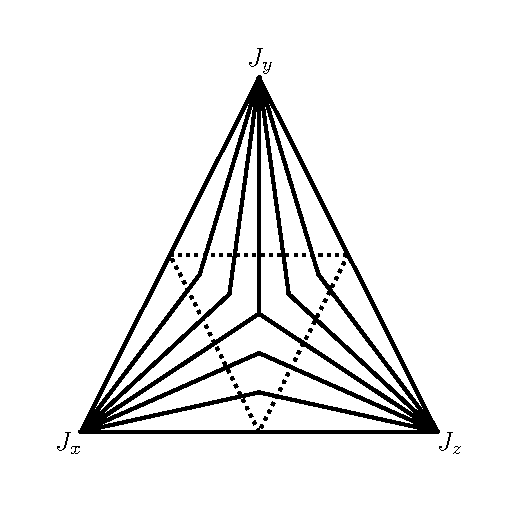
\includegraphics[width=.4\textwidth,height=.4\textheight]{figure_code/logo/logo}
\vspace{-0.4\textheight}
\vspace{10mm}
}
\submitdate{June 2022}

% \normallinespacing

\maketitle

\preface
\addcontentsline{toc}{chapter}{Abstract}

\begin{abstract}

 FK Model: Disorder or interactions can turn metals into insulators. One of the simplest settings to study this physics is given by the \ac{FK} model, which describes itinerant fermions interacting with a classical Ising background field. Despite the translational invariance of the model, inhomogenous configurations of the background field give rise to effective disorder physics which lead to a rich phase diagram in two (or more) dimensions with finite temperature charge density wave (CDW) transitions and interaction-tuned Anderson versus Mott localized phases. Here, we propose a generalised \ac{FK} model in one dimension with long-range interactions which shows a similarly rich phase diagram. We use an exact Markov Chain Monte Carlo method to map the phase diagram and compute the energy resolved localisation properties of the fermions. We compare the behaviour of this transitionally invariant model to an Anderson model of uncorrelated binary disorder about a background CDW field which confirms that the fermionic sector only fully localizes for very large system sizes.
 
 Amorphous Kitaev: 

\end{abstract}
The copyright of this thesis rests with the author. Unless otherwise indicated, its contents are licensed under a Creative Commons Attribution-Non Commercial 4.0 International Licence (CC BY-NC).

Under this licence, you may copy and redistribute the material in any medium or format. You may also create and distribute modified versions of the work. This is on the condition that: you credit the author and do not use it, or any derivative works, for a commercial purpose.

When reusing or sharing this work, ensure you make the licence terms clear to others by naming the licence and linking to the licence text. Where a work has been adapted, you should indicate that the work has been changed and describe those changes.

Please seek permission from the copyright holder for uses of this work that are not included in this licence or permitted under UK Copyright Law.

% \cleardoublepage
% \addcontentsline{toc}{chapter}{Acknowledgements}
% \begin{acknowledgements}
% I would like to thank my supervisor, Professor Johannes Knolle and co-supervisor Professor Derek Lee for guidance and support during this long process.

Dan Hdidouan for being an example of how to weather the stress of a PhD with grace and kindness.

Arnaud for help and guidance\ldots{}

Carolyn, Juraci, Ievgeniia and Loli for their patience and support.

Nina del Ser

Brian Tam for his endless energy on our many many calls while we served as joint Postgraduate reps for the department.

All the students in CMTH, Halvard, Tom, Chris, Krishnan, David, Tonny, Emanuele \ldots{} and particularly to Thank you to the CMT group at TUM in Munich, Alex and Rohit.

Gino, Peru and Willian for their collaboration on the Amorphous Kitaev Model.

Mr Jeffries who encouraged me to pursue physics

All the gang from Munich, Toni, Mine, Mike, Claudi.

Dan Simpson, the poet in residence at Imperial and one of my favourite collaborators during my time at Imperial.

Lou Khalfaoui for keeping me sane during the lockdown of March 2022. Sophie Nadel, Julie Ketcher and Kim ??? for their graphic design expertise and patience.

All the I-Stemm team, Katerina, Jeremey, John, \ldots.

And finally, I'd like the thank the staff of the Camberwell Public Library where the majority of this thesis was written.

% \end{acknowledgements}
% \include{0_Preface/personal_contributions}

\body
% \chapter{Introduction}
% One of the most interesting and perhaps surprising features of many body
physics is the existence of distinct phases of matter.

Why does liquid turn to ice? Well there are two key ingredients. First
we need a system composed of a large number of objects and second we
need those objects to interact with eachother.

It turns out that the more objects there are, the greater the effect
that their interactions has on the whole. A hundred \(H_2O\) molecules
can't actually form the nice regular structure that characterises ice,
instead you'd get more of a blob. However, any human scale amount of
water contains an unimaginable huge number of molecules.

Phases come about when the interactions between individuals components
serve the reinforce

When a many body, interacting system can display radically different
properties depending on the system parameters

\hypertarget{themes}{%
\subsection{Themes}\label{themes}}

\begin{itemize}
\item
  many body
\item
  interactions
\item
  quantum
\item
  topology
\item
  disorder
\item
  quasiparticles
\item
  topological order
\item
  protected edge states
\item
  abelian and non-abelian anyons
\item
  localisation
\item
  lengthscales
\end{itemize}

\begin{Shaded}
\begin{Highlighting}[]
\NormalTok{\_\_ Connection between }
\end{Highlighting}
\end{Shaded}


% \chapter{The Long-Range Falikov-Kimball Model}
% \hypertarget{contributions}{%
\section{Contributions}\label{contributions}}

This material is this chapter expands on work presented in

\autocite{citekey} \href{https://link.aps.org/doi/10.1103/PhysRevB.104.045116}{One-dimensional long-range Falikov-Kimball model: Thermal phase transition and disorder-free localization}, Hodson, T. and Willsher, J. and Knolle, J., Phys. Rev.~B, \textbf{104}, 4, 2021,

Johannes had the initial idea to use a long range Ising term to stablise order in a one dimension Falikov-Kimball model. Josef developed a proof of concept during a summer project at Imperial. The three of us brought the project to fruition.

\begin{Shaded}
\begin{Highlighting}[]
\NormalTok{[WARNING] Citeproc: citation abanin\_recent\_2017 }\KeywordTok{not}\NormalTok{ found abaninRecentProgressManybody2017}
\NormalTok{[WARNING] Citeproc: citation anderson\_absence\_1958}\OperatorTok{{-}}\DecValTok{1} \KeywordTok{not}\NormalTok{ found andersonAbsenceDiffusionCertain1958}
\NormalTok{[WARNING] Citeproc: citation antipov\_interaction}\OperatorTok{{-}}\NormalTok{tuned\_2016}\OperatorTok{{-}}\DecValTok{1} \KeywordTok{not}\NormalTok{ found andersonAbsenceDiffusionCertain1958}
\NormalTok{[WARNING] Citeproc: citation binder\_finite\_1981 }\KeywordTok{not}\NormalTok{ found binderFiniteSizeScaling1981}
\NormalTok{[WARNING] Citeproc: citation croy\_anderson\_2011 }\KeywordTok{not}\NormalTok{ found croyAndersonLocalization1D2011}
\NormalTok{[WARNING] Citeproc: citation dalessio\_quantum\_2016 }\KeywordTok{not}\NormalTok{ found dalessioQuantumChaosEigenstate2016}
\NormalTok{[WARNING] Citeproc: citation dyson\_existence\_1969 }\KeywordTok{not}\NormalTok{ found dysonExistencePhasetransitionOnedimensional1969}
\NormalTok{[WARNING] Citeproc: citation fig:binder }\KeywordTok{not}\NormalTok{ found}
\NormalTok{[WARNING] Citeproc: citation goldshtein\_pure\_1977 }\KeywordTok{not}\NormalTok{ found goldshteinPurePointSpectrum1977}
\NormalTok{[WARNING] Citeproc: citation huang\_accelerated\_2017 }\KeywordTok{not}\NormalTok{ found huangAcceleratedMonteCarlo2017}
\NormalTok{[WARNING] Citeproc: citation hubbard\_j.\_electron\_1963 }\KeywordTok{not}\NormalTok{ found}
\NormalTok{[WARNING] Citeproc: citation imbrie\_diagonalization\_2016 }\KeywordTok{not}\NormalTok{ found}
\NormalTok{[WARNING] Citeproc: citation imbrie\_many}\OperatorTok{{-}}\NormalTok{body\_2016 }\KeywordTok{not}\NormalTok{ found}
\NormalTok{[WARNING] Citeproc: citation izrailev\_anomalous\_2012 }\KeywordTok{not}\NormalTok{ found}
\NormalTok{[WARNING] Citeproc: citation izrailev\_localization\_1999 }\KeywordTok{not}\NormalTok{ found}
\NormalTok{[WARNING] Citeproc: citation kapfer\_sampling\_2013 }\KeywordTok{not}\NormalTok{ found}
\NormalTok{[WARNING] Citeproc: citation kennedy\_itinerant\_1986 }\KeywordTok{not}\NormalTok{ found}
\NormalTok{[WARNING] Citeproc: citation khatami\_fluctuation}\OperatorTok{{-}}\NormalTok{dissipation\_2013 }\KeywordTok{not}\NormalTok{ found}
\NormalTok{[WARNING] Citeproc: citation kramer\_localization\_1993 }\KeywordTok{not}\NormalTok{ found}
\NormalTok{[WARNING] Citeproc: citation krauth\_introduction\_1996 }\KeywordTok{not}\NormalTok{ found}
\NormalTok{[WARNING] Citeproc: citation lieb\_absence\_1968 }\KeywordTok{not}\NormalTok{ found}
\NormalTok{[WARNING] Citeproc: citation lipkin\_validity\_1965 }\KeywordTok{not}\NormalTok{ found}
\NormalTok{[WARNING] Citeproc: citation maska\_thermodynamics\_2006}\OperatorTok{{-}}\DecValTok{1} \KeywordTok{not}\NormalTok{ found}
\NormalTok{[WARNING] Citeproc: citation musial\_monte\_2002 }\KeywordTok{not}\NormalTok{ found}
\NormalTok{[WARNING] Citeproc: citation nagaoka\_ferromagnetism\_1966 }\KeywordTok{not}\NormalTok{ found}
\NormalTok{[WARNING] Citeproc: citation noauthor\_hubbard\_2013 }\KeywordTok{not}\NormalTok{ found}
\NormalTok{[WARNING] Citeproc: citation peierls\_isings\_1936 }\KeywordTok{not}\NormalTok{ found}
\NormalTok{[WARNING] Citeproc: citation roberts\_weak\_1997 }\KeywordTok{not}\NormalTok{ found}
\NormalTok{[WARNING] Citeproc: citation ruelle\_statistical\_1968 }\KeywordTok{not}\NormalTok{ found}
\NormalTok{[WARNING] Citeproc: citation schiulaz\_dynamics\_2015 }\KeywordTok{not}\NormalTok{ found}
\NormalTok{[WARNING] Citeproc: citation smith\_disorder}\OperatorTok{{-}}\NormalTok{free\_2017 }\KeywordTok{not}\NormalTok{ found}
\NormalTok{[WARNING] Citeproc: citation smith\_dynamical\_2018 }\KeywordTok{not}\NormalTok{ found}
\NormalTok{[WARNING] Citeproc: citation srednicki\_chaos\_1994 }\KeywordTok{not}\NormalTok{ found}
\NormalTok{[WARNING] Citeproc: citation thouless\_long}\OperatorTok{{-}}\NormalTok{range\_1969 }\KeywordTok{not}\NormalTok{ found}
\NormalTok{[WARNING] Citeproc: citation yao\_quasi}\OperatorTok{{-}}\NormalTok{many}\OperatorTok{{-}}\NormalTok{body\_2016 }\KeywordTok{not}\NormalTok{ found}
\end{Highlighting}
\end{Shaded}

\hypertarget{introduction}{%
\section{Introduction}\label{introduction}}

\hypertarget{localisation}{%
\subsection{Localisation}\label{localisation}}

The discovery of localisation in quantum systems surprising at the time given the seeming ubiquity of extended Bloch states. Later, when thermalisation in quantum systems gained interest, localisation phenomena again stood out as counterexamples to the eigenstate thermalisation hypothesis \autocite{abanin_recent_2017,srednicki_chaos_1994}, allowing quantum systems to avoid to retain memory of their initial conditions in the face of thermal noise.

The simplest and first discovered kind is Anderson localisation, first studied in 1958 \textcite{anderson_absence_1958-1} in the context of non-interacting fermions subject to a static or quenched disorder potential \(V_j\) drawn uniformly from the interval \([-W,W]\)

\[
H = -t\sum_{\langle jk \rangle} c^\daggerger_j c_k + \sum_j V_j c_j^\daggerger c_j
\]

this model exhibits exponentially localised eigenfunctions \(\psi(x) = f(x) e^{-x/\lambda}\) which cannot contribute to transport processes. Initially it was thought that in one dimensional disordered models, all states would be localised, however it was later shown that in the presence of correlated disorder, bands of extended states can exist \autocite{izrailev_localization_1999,croy_anderson_2011,izrailev_anomalous_2012}.

Later localisation was found in interacting many-body systems with quenched disorder:

\[
H = -t\sum_{\langle jk \rangle} c^\daggerger_j c_k + \sum_j V_j c_j^\daggerger c_j + U\sum_{jk} n_j n_k
\]

where the number operators \(n_j = c^\dagger_j c_j\). Here, in contrast to the Anderson model, localisation phenomena can be proven robust to weak perturbations of the Hamiltonian. This is called many-body localisation (MBL) \textcite{imbrie_many-body_2016}.

Both MBL and Anderson localisation depend crucially on the presence of quenched disorder. This has led to ongoing interest in the possibility of disorder-free localisation, in which the disorder necessary to generate localisation is generated entirely from the dynamics of the model. This contracts with typical models of disordered systems in which disorder is explicielty introduced into the Hamilton or the initial state.

The concept of disorder-free localisation was first proposed in the context of Helium mixtures \textcite{kagan1984localization} and then extended to heavy-light mixtures in which multiple species with large mass ratios interact. The idea is that the heavier particles act as an effective disorder potential for the lighter ones, inducing localisation. Two such models \autocite{yao_quasi-many-body_2016,schiulaz_dynamics_2015} instead find that the models thermalise exponentially slowly in system size, which Ref. \textcite{yao_quasi-many-body_2016} dubs Quasi-MBL.

True disorder-free localisation does occur in exactly solveable models with extensively many conserved quantities \textcite{smith_disorder-free_2017}. As conserved quantites have no time dynamics this can be thought of as taking the separation of timescales to the infinite limit.

\hypertarget{the-falikov-kimball-model}{%
\subsubsection{The Falikov Kimball Model}\label{the-falikov-kimball-model}}

In the Falikov Kimball (FK) model spinless fermions \(c_{i\uparrow}\) are coupled via a repulsive on-site interaction to a classical degree of freedom \(n_{i\downarrow}\).

\[\begin{aligned}
H &= -t \sum_{<ij>} c^\daggerger_{i\uparrow}c_{j\uparrow} + U \sum_{i} (n_{i \uparrow} - 1/2)( n_{i\downarrow} - 1/2) \\
       & - \mu \sum_i \left( n_{i \uparrow} + n_{i \downarrow} \right) + \sum_{ij} V_{ij} (n_{i\downarrow} - 1/2)(n_{j\downarrow} - 1/2) 
\end{aligned}\] \textbf{replace with hamiltonian from the paper}

This notation emphasises that this can also be thought of as an asymmetric Hubbard model in which the spin down electrons cannot hop and are subject to an additional long range potential. However, to avoid the confusion of talking about two distinct species of spinless electrons we will use a different interpretation and refer to the classical degrees of freedom as the ``ionic sector'' and the quantum degrees of freedom as the ``electronic sector''. The final term that induces interactions between the classical particles has been added by us to stabilise the formation of an ordered phase in 1D. The classical variables commute with the Hamiltonian \([H, n_{i\downarrow}] = 0\) so like the lattice gauge model in Ref \textcite{smith_disorder-free_2017}\} the FK model has extensively many conserved quantities which can act as an effective disorder potential for the electronic sector.

Due to Pauli exclusion, the maximum filling occurs when one of each species occupies each lattice site such that \(\sum_i (n_{i\downarrow} + n_{i\uparrow} )/ N = 2\). Here we focus on the half filled case which also displays particle-hole symmetry (see later).

\hypertarget{falikov-kimball-and-hubbard-models}{%
\subsection{Falikov Kimball and Hubbard models}\label{falikov-kimball-and-hubbard-models}}

We will first introduce the standard Hubbard and Falikov-Kimball (FK) models then look at some of their properties. We'll then cover why the Falikov-Kimball model represents an interesting system in which to study disorder free localisation.

\hypertarget{hubbard-model}{%
\subsubsection{Hubbard model}\label{hubbard-model}}

The Hubbard model gives a very simple setting in which to study interacting, itinerant electrons. It is a tight binding model of spin half electrons with finite bandwidth \(t\) and a repulsive on-site interaction \(U > 0\).

\[
    H = -\sum_{<ij>,\sigma} t_{\sigma} c^\dagger_{i\sigma}c_{j\sigma} + U \sum_{i} (n_{i \uparrow} - 1/2)( n_{i\downarrow} - 1/2) - \mu \sum_i \left( n_{i \uparrow} + n_{i \downarrow} \right)
\]

in standard notation. The standard Hubbard model corresponds to the case \(t_{\uparrow} = t_{\downarrow}\). Here we have used the particle-hole symmetric version of the interaction term, which is more often given as \(n_{i \uparrow} n_{i\downarrow}\). The difference just amounts to a redefinition of the chemical potential.

Hubbard originally used the model at half filling \(\mu = 0\) to explain the Mott metal-insulator (MI) transition, however it has seen applications to high-temperature superconductivity and become target for cold-atom optical trap experiments. \textcite{noauthor_hubbard_2013}, greiner\_quantum\_2002, jordens\_mott\_2008\}. While simple, only a few analytic results exist, namely the Bethe ansatz \textcite{lieb_absence_1968}\} which proves the absence of even a zero temperature phase transition in the 1D model and Nagaoka's theorem \textcite{nagaoka_ferromagnetism_1966}\} which proves that the three dimensional model has a ferromagnetic ground state in the vicinity of half filling.

\hypertarget{falikov-kimball-model}{%
\subsubsection{Falikov-Kimball model}\label{falikov-kimball-model}}

\begin{figure}
  \centering
    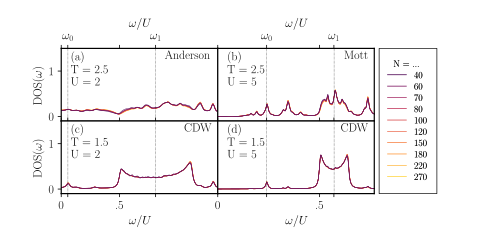
\includegraphics[width=\textwidth]{figs/DOS}
  \caption{Density of states for the Anderson model with (a) no potential, (b) a charge density wave (CDW) potential $\vec{h} = (0,1,0,1...)$, (c) a disordered CDW potential each site has an uncorrelated $2\%$ chance of deviating from the CDW background. Hopping and potential terms both have unit magnitude.}
  \label{fig:fk_dos}
\end{figure}

The Falikov-Kimball model corresponds to the case \(t_{\downarrow} = 0\). It can be interpreted as two coupled spinless electron bands with infinite mass ratio. An itinerant light species with creation operator \(c^\dagger_{i\uparrow}\) coupled to an infinitely heavy, immobile species with density operator \(n_{i\downarrow}\). These are often called c and f electrons or electrons and ions. The model was first introduced by Hubbard in 1963 as a model of interacting localised and de-localised electron bands and gained its name from Falikov and Kimball's use of it to study the MI transition in rare-earth materials \textcite{hubbard_j._electron_1963}, falicov\_simple\_1969\}.

Here we will use refer to the light spinless species as \texttt{electrons\textquotesingle{}\ with\ creation\ operator\ \$c\^{}\textbackslash{}dagger\_\{i\}\$\ and\ the\ heavy\ species\ as}ions' with density operator \(n_i\). When the the density operator of the electrons is needed I'll always use \(c^\dagger_{i}c_{i}\). We also set \(t = 1\).

\[
    H_{\mathrm{FK}} = -\sum_{<ij>} c^\dagger_{i}c_{j} + U \sum_{i} (c^\dagger_{i}c_{i} - 1/2)( n_i - 1/2) - \mu \sum_i \left(c^\dagger_{i}c_{i} + n_{i}\right)
\] \% \#\#\# Particle-Hole Symmetry The Hubbard and FK models on a bipartite lattice have particle-hole (PH) symmetry \(P^\dagger H P = - H\), accordingly they have symmetric energy spectra. The associated symmetry operator \(P\) exchanges creation and annihilation operators along with a sign change between the two sublattices.

\[ d^\dagger_{i\sigma} = (-1)^i c_{i\sigma}\] \% The entirely filled state \(\ket{\Omega} = \sum_{j\rho} c^\dagger_{j\rho} \ket{0}\) becomes the new vacuum state: \[d_{i\sigma} \ket{\Omega} = (-1)^i c^\dagger_{i\sigma} \sum_{j\rho} c^\dagger_{j\rho} \ket{0} = 0\] \% The number operator \(n_{i\sigma} = 0,1\) counts holes rather than particles: \[ d^\dagger_{i\sigma} d_{i \sigma} = c_{i\sigma} c^\dagger_{i\sigma} = 1 - c^\dagger_{i\sigma} c_{i\sigma}\] \% With the last equality following from the fermionic commutation relations. In the case of nearest neighbour hopping on a bipartite lattice this transformation also leaves the hopping term unchanged: \[ d^\dagger_{i\sigma} d_{j \sigma} = (-1)^{i+j} c_{i\sigma} c^\dagger_{j\sigma} = c^\dagger_{i\sigma} c_{j\sigma} \] \% Since when \(i\) and \(j\) label sites on separate sublattices, \((-1)^{i-j} = -1\) and this is absorbed into rearranging the operators via their anti-commutator.

Defining the particle density \(\rho\) as the number of fermions per site: \[
    \rho = \frac{1}{N} \sum_i \left( n_{i \uparrow} + n_{i \downarrow} \right)
\] \% The PH symmetry maps the Hamiltonian to itself with the sign of the chemical potential reversed and the density is inverted about half filling: \[ \text{PH} : H(t, U, \mu) \rightarrow H(t, U, -\mu) \] \[ \rho \rightarrow 2 - \rho \] \% The Hamiltonian is symmetric under PH at \(\mu = 0\) and so must all the observables, hence half filling \(\rho = 1\) occurs here. This symmetry and known observable acts as a useful test for the numerical calculations.

\hypertarget{thermodynamics-of-the-fk-model}{%
\subsubsection{Thermodynamics of the FK model}\label{thermodynamics-of-the-fk-model}}

\textbackslash begin\{figure\} \centering 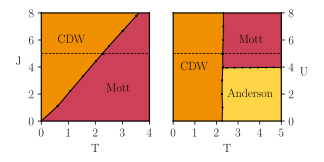
\includegraphics[width=0.8\textwidth]{figs/phase_diagram}

\caption{Phases of the 2D Falikov Kimball Model, showing the ordered charge density wave phase at low temperatures and the interaction mediated transition between Anderson localisation and Mott insulating phases in the disordered phase. @antipov_interaction-tuned_2016-1}

\} \label{fig:FK_phase_diagram} \textbackslash end\{figure\}

At half filling and in dimensions greater than one, the FK model exhibits a phase transition at some \(U\) dependent critical temperature \(T_c(U)\) to a low temperature charge density wave state in which the ions occupy one of the two sublattices A and B \textcite{maska_thermodynamics_2006-1}\}. The order parameter is the square of the staggered magnetisation: \[
M = \sum_{i \in A} n_i - \sum_{i \in B} n_i
\] \% In the disordered phase Ref. \textcite{antipov_interaction-tuned_2016-1}\} identifies an interplay between Anderson localisation at weak interaction and a Mott insulator phase in the strongly interacting regime.

In the one dimensional FK model, however, Peierls' argument \textcite{peierls_isings_1936}, kennedy\_itinerant\_1986\} and the Bethe ansatz \textcite{lieb_absence_1968}\} make it clear that there is no ordered CDW phase. Peierls' argument is that one should consider the difference in free energy \(\Delta F = \Delta E - T\Delta S\) between an ordered state and a state with single domain wall in the order parameter. In the Ising model this would be having the spins pointing up in one part of the model and down in the other, for a CDW phase it means having the ions occupy the A sublattice in one part and the B sublattice in the other.

Short range interactions will produce a constant energy penalty for such a domain wall that does not scale with system size while in 1D there are \(L\) such states so the domain wall is associated with entropy \(S \propto \ln L\) which dominates in the thermodynamic limit. The slow logarithmic scaling suggests we should be wary of finite size scaling effects.

One dimensional systems are more amenable to numerical and experimental study so we add long range staggered interactions to bring back the ordered phase:

\[ H_{\textrm{int}} = 4J \sum_{ij} \frac{(-1)^{|i-j|}}{ |i - j|^{\alpha} } (n_i - 1/2) (n_j - 1/2) = J \sum_{ij} |i - j|^{-\alpha} \tau_i \tau_j\] \% at half-filling the modified Hamiltonian is then: \[
    H_{\mathrm{FK}}^* &= -\sum_{<ij>} c^\dagger_{i}c_{j} + U \sum_{i} (c^\dagger_{i}c_{i} - 1/2)( n_i - 1/2) \\
    &+ 4J \sum_{ij} \frac{(-1)^{|i-j|}}{ |i - j|^{\alpha} } (n_i - 1/2) (n_j - 1/2)  \\
    &= -\sum_{<ij>} c^\dagger_{i}c_{j} + 2U \sum_{i} (-1)^i (c^\dagger_{i}c_{i} - 1/2)\tau_i + J \sum_{ij} |i - j|^{-\alpha} \tau_i \tau_j  \\
\] \% The form of this interaction comes from interpreting the f-electrons as a classical Ising chain using a staggered mapping \(\tau_i = (-1)^i (2n_i^ f - 1)\) so that ferromagnetic order in the \(\tau_i\) variables corresponds to a CDW state in the \(n_i^f\) variables. It also preserves the particle hole symmetry because for the ions the PH transformation corresponds to \(n_i \rightarrow 1 - n_i\). When \(U = 0\) the model decouples into a long ranged Ising model and free fermions.

\subsubsection{Long Ranged Ising model}

Our extension to the FK model could now be though of as spinless fermions coupled to a long range Ising (LRI) model. The LRI model has been extensively studied and its behaviour may be bear relation to the behaviour of our modified FK model.

\[H_{\mathrm{LRI}} = \sum_{ij} J(\abs{i-j}) \tau_i \tau_j = J \sum_{i\neq j} |i - j|^{-\alpha} \tau_i \tau_j\] \% Rigorous renormalisation group arguments show that the LRI model has an ordered phase in 1D for \$1 \textless{} \alpha \textless{} 2 \$ \textcite{dyson_existence_1969}\}. Peierls' argument can be extended \textcite{thouless_long-range_1969}\} to provide intuition for why this is the case. Again considering the energy difference between the ordered state \(\ket{\ldots\uparrow\uparrow\uparrow\uparrow\ldots}\) and a domain wall state \(\ket{\ldots\uparrow\uparrow\downarrow\downarrow\ldots}\). In the case of the LRI model, careful counting shows that this energy penalty is: \[\Delta E \propto \sum_{n=1}^{\infty} n J(n)\] \% because each interaction between spins separated across the domain by a bond length \(n\) can be drawn between \(n\) equivalent pairs of sites. Ruelle proved rigorously for a very general class of 1D systems, that if \(\Delta E\) or its many-body generalisation converges in the thermodynamic limit then the free energy is analytic \textcite{ruelle_statistical_1968}\}. This rules out a finite order phase transition, though not one of the Kosterlitz-Thouless type. Dyson also proves this though with a slightly different condition on \(J(n)\) \textcite{dyson_existence_1969}\}.

With a power law form for \(J(n)\), there are three cases to consider:

\begin{center}
    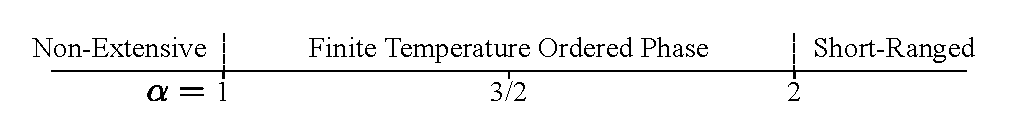
\includegraphics[width=\textwidth]{figs/alpha_diagram}
\end{center}

\begin{enumerate}
\def\labelenumi{\arabic{enumi}.}
\tightlist
\item
  \$ \alpha = 0\$ For infinite range interactions the Ising model is exactly solveable and mean field theory is exact \textcite{lipkin_validity_1965}\}.
\item
  \$ \alpha \le 1\$ For slowly decaying interactions \(\sum_n J(n)\) does not converge so the Hamiltonian is non-extensive, a case which won't be further considered here.
\item
  \$ 1 \textless{} \alpha \textless{} 2 \$ A phase transition to an ordered state at a finite temperature.
\item
  \$ \alpha = 2 \$ The energy of domain walls diverges logarithmically, and this turns out to be a Kostelitz-Thouless transition \textcite{thouless_long-range_1969}\}.
\item
  \$ 2 \textless{} \alpha \$ For quickly decaying interactions, domain walls have a finite energy penalty, hence Peirels' argument holds and there is no phase transition.
\end{enumerate}

\hypertarget{thermodynamics}{%
\subsubsection{Thermodynamics}\label{thermodynamics}}

On bipartite lattices in dimensions 2 and above the FK model exhibits a finite temperature phase transition to an ordered charge density wave (CDW) phase \textcite{maska_thermodynamics_2006-1}. In this phase, the ions are confined to one of the two sublattices, breaking the \(\mathbb{Z}_2\) symmetry.

In 1D, however, Periel's argument \autocite{peierls_isings_1936,kennedy_itinerant_1986} states that domain walls only introduce a constant energy penalty into the free energy while bringing a entropic contribution logarithmic in system size. Hence the 1D model does not have a finite temperature phase transition. However 1D systems are much easier to study numerically and admit simpler realisations experimentally. We therefore introduce a long range coupling between the ions in order to stabilise a CDW phase in 1D. This leads to a disordered system that is gaped by the CDW background but with correlated fluctuations leading to a disorder-free correlation induced mobility edge in one dimension.

\hypertarget{markov-chain-monte-carlo}{%
\subsubsection{Markov Chain Monte Carlo}\label{markov-chain-monte-carlo}}

To evaluate thermodynamic averages we perform a classical Markov Chain Monte Carlo random walk over the space of ionic configurations, at each step diagonalising the effective electronic Hamiltonian \textcite{maska_thermodynamics_2006-1}\}. Using a binder-cumulant method \autocite{binder_finite_1981,musial_monte_2002}, we demonstrate the model has a finite temperature phase transition when the interaction is sufficiently long ranged. We then estimate the density of states and the inverse participation ratio as a function of energy to diagnose localisation properties. We show preliminary results that the in-gap states induced at finite temperature are localised while the states in the unperturbed bands remain extended, evidence for a mobility edge.

\begin{figure}
\hypertarget{fig:binder}{%
\centering
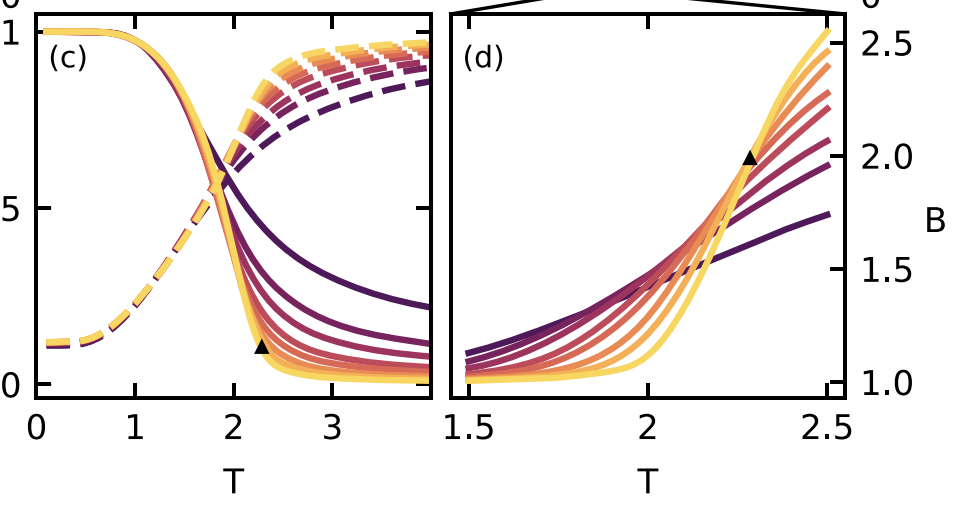
\includegraphics[width=1\textwidth,height=\textheight]{figure_code/fk_chapter/binder.png}
\caption{Hello I am the figure caption!}\label{fig:binder}
}
\end{figure}

Macro definitions in this cell \[
\newcommand{\expval}[1]{\langle #1 \rangle}
\newcommand{\ket}[1]{|#1\rangle}
\newcommand{\bra}[1]{\langle#1|}
\newcommand{\op}[2]{|#1\rangle \langle#2|}
\]

\[
\expval{O}, \op{\alpha}{\beta}, \ket{\psi}
\]

\hypertarget{localisation-1}{%
\subsection{Localisation}\label{localisation-1}}

\hypertarget{thermalisation}{%
\subsubsection{Thermalisation}\label{thermalisation}}

Isolated classical systems generally thermalise if they are large enough. Since classical dynamics is the limit of some underlying quantum dynamics, it seems reasonable to suggest that isolated quantum systems also thermalise in some related sense. However it is not immediately obvious what thermalisation should mean in a quantum setting where the presence of unitary time dynamics implies full information about a system's initial state is always preserved.

A potential solution lies in the eigenstate thermalisation hypothesis. It states that if a system thermalises, then we can isolate small patches of a larger system, trace everyhing else out, and get a thermal density matrix.

Following Ref. \textcite{abanin_recent_2017}, consider the time evolution of a local operator \(\hat{O}\) \[ \expval{\hat{O}}{\psi(t)} = \sum_{\alpha \beta} C^*_\alpha C_\beta e^{i(E_\alpha - E_\beta)} O_{\alpha \beta}\]

Where \(C_\alpha\) are determined by the initial state and \(O_{\alpha \beta} = \expval{\alpha | \hat{O} | \beta}\) are the matrix elements of \(\hat{O}\) with respect to the energy eigenstates. Srednicki \textcite{srednicki_chaos_1994}\} introduced the ansatz that for local operators:

\[O_{\alpha \beta} = O(E)\delta_{\alpha\beta} + e^{-S(E)/2} f(E,\omega) R_{\alpha\beta}\]

with \(E = (E_\alpha + E_\beta)\), \(\omega = (E_\alpha - E_\beta)\) and \(R_{\alpha\beta}\) are sampled from some distribution with zero mean and unit variance. The first term asserts that the diagonal elements are given by the thermal expectation value \(O(E) = Tr[e^{-\beta \hat{H}} \hat{O}]/\mathcal{Z}\) with \(\beta\) an effective temperature defined by equating the energy to the expectation of the Hamiltonian at that temperature \(E = Tr[H e^{-\beta \hat{H}}/\mathcal{Z}]\).

The second term deals with thermodynamic fluctuations scaled by the entropy \(S(E) = -Tr(\rho \log \rho)\) where \(\rho = e^{-\beta \hat{H}}\) and \(\mathcal{Z} = Tr[e^{-\beta \hat{H}}]\).

With this ansatz the long time average of the observable becomes equal to the thermal expectations with fluctuations suppressed by the entropic term \(e^{-S(E)}\) and the rapidly varying phase factors \(e^{i(E_\alpha - E_\beta)}\). This statement of the ETH has verified for the quantum hard sphere model \textcite{srednicki_chaos_1994} and numerically for other models \autocite{khatami_fluctuation-dissipation_2013,dalessio_quantum_2016}.

An alternate view on ETH is the statement that in thermalising systems individual eigenstates look thermal when viewed locally. Take a eigenstate \(|\alpha\rangle\) with energy \(E_\alpha\) and as before define an effective temperature with \(E_\alpha = Tr[H e^{-\beta \hat{H}}/\mathcal{Z}]\). This statement of the ETH says that if we partition the system into subsystems A and B with a limit taken as B becomes very large, B will act as a heat bath for A. Specifically the reduced density matrix \(\rho_A = Tr_B \op{\alpha}{\alpha}\) is equal to the thermal density matrix:

\[\rho_A = Tr_B |\alpha\rangle \langle \alpha| = \mathcal{Z}^{-1} Tr_B [e^{-\beta \hat{H}}] \]

Intuitively, for thermalisation to happen, the degrees of freedom must be sufficiently well coupled that energy transport occurs. This condition is broken by systems with localised states so a lack of thermalisation is often used as a diagnostic tool for localisation.

\hypertarget{anderson-localisation}{%
\subsubsection{Anderson Localisation}\label{anderson-localisation}}

Localisation was first studied by Anderson in 1958 \textcite{anderson_absence_1958-1} in the context of non-interacting fermions subject to a static or quenched disorder potential \(V_j\) drawn uniformly from the interval \([-W,W]\):

\[
H = -t\sum_{\expval{jk}} c^\dagger_j c_k + \sum_j V_j c_j^\dagger c_j
\]

At sufficiently strong disorder the Anderson model exhibits exponentially localised eigenfunctions \(\psi(x) = f(x) e^{-x/\lambda}\) which cannot contribute to diffusive transport processes. Except in 1D where any disorder strength is sufficient. Intuitively this happens because hopping processes between nearby sites become off-resonant, hindering the hybridisation that would normally lead to extended Bloch states \textcite{kramer_localization_1993}.

In one and two dimensions, all the states in the Anderson model are localised. In three dimensions there are mobility edges. Mobility edges are critical energies in the spectrum which separate delocalised states in a band from localised states which form a band tail \textcite{abanin_recent_2017}\}. An argument due to Lifshitz shows that the density of state of the band tail should decay exponentially and localised and extended stats cannot co-exist at the same energy as they would hybridise into extended states \textcite{kramer_localization_1993}\}.

It was thought that mobility edges could not exist in 1D because all the states localised in the presence of any amount of disorder. This is true for uncorrelated potentials \textcite{goldshtein_pure_1977}\}. However, it was shown that if the disorder potential \(V_j\) contains spatial correlations mobility edges do exist in 1D \textcite{izrailev_localization_1999}, izrailev\_anomalous\_2012\}. Ref. \textcite{croy_anderson_2011}\} extends this work to look at power law decay of the correlations: \[ C(l) = \expval{V_i V_{i+l}} \propto l^{-\alpha} \] \% Figure \ref{fig:anderson_dos} shows numerical calculations of the Localisation length (see later) and density of states for the power law correlated Anderson model. At the unperturbed band edges \(\abs{E} = 2\), the states transition from extended to localised. The behaviour close to the edge takes a universal scaling form with exponents dependant on \(\alpha\).

\hypertarget{many-body-localisation}{%
\subsubsection{Many Body Localisation}\label{many-body-localisation}}

A related phenomena known as many body localisation (MBL) was found in interacting systems with quenched disorder. A simple example comes from adding density-density interactions to the Anderson model:

\[
H = -t\sum_{\expval{jk}} c^\dagger_j c_k + \sum_j V_j c_j^\dagger c_j + U\sum_{jk} n_j n_k
\] \% with \(n_j = c^\dagger_j c_j\) Here, in contrast to the Anderson model, localisation phenomena can be proven robust to weak perturbations of the Hamiltonian \textcite{imbrie_many-body_2016}\}.

MBL is defined by the emergence of an extensive number of quasi-local operators called local integrals of motions (LIOMs) or l-bits. Following Ref. \textcite{abanin_recent_2017}\}, using a spin system with variables \(\sigma^z_i\), any operator can be written in the general form:

\[ \tau^z_i = \sigma^z_i + \sum_{\alpha\beta kl} f_{kl}^{\alpha\beta} \sigma^\alpha_{i+k} \sigma_z\beta_{i+k} + ...\] \% what defines a MBL system is that there exist extensively many \(\tau^z_i\) for which the coefficients decay exponentially with distance \(f_{kl}^{\alpha\beta} \propto e^{-\max(\abs{l},\abs{k}) / \xi}\). These LIOMs commute with the Hamiltonian and each other \([\hat{H}, \tau^z_i] = [\tau^z_i, \tau^z_j] = 0\). It is this extensive number of conserved local charges that leads to the localisation properties of MBL. It also has implications for the way entanglement grows over time in MBL systems.

Since the Hamiltonian commutes with all the LIOMs and they are a complete operator basis, the Hamiltonian can be written as:

\[\hat{H} = \sum_{i} h_i \tau^z_i + \sum_{ij} J_{ij} \tau^z_i \tau^z_j + \sum_{ijk} J_{ij} \tau^z_i \tau^z_j \tau^z_k+ ...\] \% Where again the couplings decay exponentially, albeit with a different length scale \(\Bar{\xi}\). From this form we see that distant l-bits can only become entangled on a timescale of:

\[ t_{\mathrm{ent}}(r) \propto \frac{\hbar}{J_0} e^{r/\Bar{\xi}} \] \% and hence quantum correlations and entanglement propagates logarithmically in MBL systems \textcite{imbrie_diagonalization_2016}\}.

\hypertarget{disorder-free-localisation}{%
\subsubsection{Disorder Free localisation}\label{disorder-free-localisation}}

Both Anderson localisation and MBL depend on the presence of quenched disorder. Recently the idea of disorder-free localisation has gained traction, asking whether the disorder necessary to generate localisation can be generated entirely from the dynamics of a model itself.

The idea was first proposed in the context of Helium mixtures \textcite{kagan1984localization}\} and then extended to heavy-light mixtures in which multiple species with large mass ratios interact, the idea being that the heavier particles act as an effective disorder potential for the lighter ones, inducing localisation. Two such models \textcite{yao_quasi-many-body_2016},schiulaz\_dynamics\_2015\} instead find that the models thermalise exponentially slowly in system size, which Ref. \textcite{yao_quasi-many-body_2016}\} dubs Quasi-MBL. A. Smith, J. Knolle et al instead looked at models containing an extensive number of conserved quantities and demonstrated true disorder free localisation \textcite{smith_disorder-free_2017}\}.

\hypertarget{diagnostics-of-localisation}{%
\subsubsection{Diagnostics of Localisation}\label{diagnostics-of-localisation}}

\hypertarget{inverse-participation-ratio}{%
\paragraph{Inverse Participation Ratio}\label{inverse-participation-ratio}}

The inverse participation ratio is defined for a normalised wave function \(\psi_i = \psi(x_i), \sum_i \abs{\psi_i}^2 = 1\) as its fourth moment \textcite{kramer_localization_1993}\}: \[
P^{-1} = \sum_i \abs{\psi_i}^4
\] \% It acts as a measure of the portion of space occupied by the wave function. For localised states it will be independent of system size while for plane wave states in d dimensions \$P = L\^{}d \$. States may also be intermediate between localised and extended, described by their fractal dimensionality \(d > d* > 0\): \[
P(L) \goeslike L^{d*} 
\] \% For extended states \(d* = 0\) while for localised ones \(d* = 0\). In this work we take use an energy resolved IPR \textcite{antipov_interaction-tuned_2016-1}: \[
DOS(\omega) = \sum_n \delta(\omega - \epsilon_n)
IPR(\omega) = DOS(\omega)^{-1} \sum_{n,i} \delta(\omega - \epsilon_n) \abs{\psi_{n,i}}^4
\] Where \(\psi_{n,i}\) is the wavefunction corresponding to the energy \(\epsilon_n\) at the ith site. In practice we bin the energies and IPRs into a fine energy grid and use Lorentzian smoothing if necessary.

\hypertarget{transfer-matrix-approach}{%
\paragraph{Transfer Matrix Approach}\label{transfer-matrix-approach}}

The transfer matrix method (TMM) can be used to calculate the localisation length of the eigenstates of a system. Following Refs. \textcite{kramer_localization_1993}, smith\_dynamical\_2018\}, for bi-linear, 1D Hamiltonians the method represents the action of \(H\) on a state \(\ket{\psi} = \sum_i \psi_i \ket{i}\) with energy E by a matrix equation: \[
H &= - \sum_i (c^\dagger_i c_{i+1} + c^\dagger_{i+1} c_{i}) - \sum_i h_i c^\dagger_i c_i \\
E\ket{\psi} &= H \ket{\psi} \\
\label{eq:tmm_difference} E \psi_i &= -(\psi_{i+1} + \psi_{i-1}) - h_i \psi_i 
\] \% Where Eq. \ref{eq:tmm_difference} can be represented by a matrix equation: \[
\begin{pmatrix}
\psi_{i+1}\\
\psi_{i}
\end{pmatrix}
=
\begin{pmatrix}
-(E + h_i) &  -1\\
1 & 0
\end{pmatrix}
\begin{pmatrix}
\psi_{i}\\
\psi_{i-1}
\end{pmatrix}
= T_i 
\begin{pmatrix}
\psi_{i}\\
\psi_{i-1}
\end{pmatrix}
\] \% Defining a product along the chain: \[Q_L = \prod_{i=0}^L T_i\] \% Oseledec's theorem proves that there exists a limiting matrix \(\Gamma\): \[
\Gamma = \lim_{L \to \infty} (Q_L Q_L^\dagger)^{\frac{1}{2L}}
\] \% with eigenvalues \(\exp(\gamma_i)\) where \(\gamma_i\) are the Lyapunov exponents of \(Q_L\). The smallest Lyapunov exponent is the inverse of the localisation length of the state. In practice one takes \(Q_L\) with L equal to the system size, finds the smallest eigenvalue q and estimates the localisation length by: \[
\lambda = \frac{L}{\ln{q}}
\] \% As noted by \textcite{smith_dynamical_2018} this method can be numerically unstable because the matrix elements diverge or vanish exponentially. To get around this, the authors break the matrix multiplication into chunks and the logarithms of the eigenvalues of each are stored separately.

\hypertarget{numerical-methods}{%
\subsection{Numerical Methods}\label{numerical-methods}}

In this section we will define the Markov Chain Monte Carlo (MCMC) method in general then detail its application to the FK model. We will then cover methods applicable to the measurements obtained from MCMC. These include calculation of the density of states and energy resolved inverse participation ratio as well as phase transition diagnostics such as the Binder cumulant.

\hypertarget{markov-chain-monte-carlo-1}{%
\subsubsection{Markov Chain Monte Carlo\}}\label{markov-chain-monte-carlo-1}}

Markov Chain Monte Carlo (MCMC) is a technique for evaluating thermal expectation values \(\expval{O}\) with respect to some physical system defined by a set of states \(\{x: x \in S\}\) and a free energy \(F(x)\) \textcite{krauth_introduction_1996}\}. The thermal expectation value is defined via a Boltzmann weighted sum over the entire states: \[
    \tex{O} &= \frac{1}{\Z} \sum_{x \in S} O(x) P(x) \\
    P(x) &= \frac{1}{\Z} e^{-\beta F(x)} \\
    \Z &= \sum_{x \in S} e^{-\beta F(x)}
\]

When the state space is too large to evaluate this sum directly, MCMC defines a stochastic algorithm which generates a random walk \(\{x_0\ldots x_i\ldots x_N\}\) whose distribution \(p(x_i)\) approaches a target distribution \(P(x)\) in the large N limit.

\[\lim_{i\to\infty} p(x_i) = P(x)\]

In this case the target distribution will be the thermal one \(P(x) \rightarrow \Z^{-1} e^{-\beta F(x)}\). The major benefit of the method being that as long as one can express the desired \(P(x)\) up to a multiplicative constant, MCMC can be applied. Since \(e^{-\beta F(x)}\) is relatively easy to evaluate, MCMC provides a useful method for finite temperature physics.

Once the random walk has been carried out for many steps, the expectation values of \(O\) can be estimated from the MCMC samples: \[
    \tex{O} = \sum_{i = 0}^{N} O(x_i) + \mathcal{O}(\frac{1}{\sqrt{N}})
\] The the samples in the random walk are correlated so the samples effectively contain less information than \(N\) independent samples would. As a consequence the variance is larger than the \(\tex{O^2} - \tex{O}^2\) form it would have if the estimates were uncorrelated. Methods of estimating the true variance of \(\tex{O}\) and decided how many steps are needed will be considered later.

\subsubsection{The Metropolis-Hasting Algorithm}

Markov chains are defined by a transition function \$\T(x\_\{i+1\} \rightarrow x\_i) \$ giving the probability that a chain in state \(x_i\) at time \(i\) will transition to a state \(x_{i+1}\). Since we must transition somewhere at each step, this comes with the normalisation condition that \(\sum\limits_x \T(x' \rightarrow x) = 1\).

If we define an ensemble of Markov chains and consider the distributions we get a sequence of distributions \(\{p_0(x), p_1(x), p_2(x)\ldots\}\) with \[p_{i+1}(x) &= \sum_{x' \in S} p_i(x') \T(x' \rightarrow x)\] \(p_o(x)\) might be a delta function on one particular starting state which would then be smoothed out by the transition function repeatedly.

As we'd like to draw samples from the target distribution \(P(x)\) the trick is to choose \$\T(x\_\{i+1\} \rightarrow x\_i) \$ such that :

\[
P(x) &= \sum_{x'} P(x') \T(x' \rightarrow x)
\] In other words the MCMC dynamics defined by \(\T\) must be constructed to have the target distribution as their only fixed point. This condition is called the global balance condition. Along with some more technical considerations such as ergodcity which won't be considered here, global balance suffices to ensure that a MCMC method is correct.

A sufficient but not necessary condition for global balance to hold is detailed balance:

\[
P(x) \T(x \rightarrow x') = P(x') \T(x' \rightarrow x)
\] \% In practice most algorithms are constructed to satisfy detailed balance though there are arguments that relaxing the condition can lead to faster algorithms \textcite{kapfer_sampling_2013}\}.

The goal of MCMC is then to choose \(\T\) so that it has the desired thermal distribution \(P(x)\) as its fixed point and that it converges quickly onto it. This boils down to requiring that the matrix representation of \(T_{ij} = \T(x_i \to x_j)\) has an eigenvector equal to \(P_i = P(x_i)\) with eigenvalue 1 and all other eigenvalues with magnitude less than one. The convergence time depends on the magnitude of the second largest eigenvalue.

\subsubsection{Metropolis-Hastings}

In order to actually choose new states according to \(\T\) one chooses states from a proposal distribution \(q(x_i \to x')\) that can be directly sampled from. For instance, this might mean flipping a single random spin in a spin chain, in which case \(q(x'\to x_i)\) is the uniform distribution on states reachable by one spin flip from \(x_i\). The proposal \(x'\) is then accepted or rejected with an acceptance probability \(\A(x'\to x_{i+1})\), if the proposal is rejected then \(x_{i+1} = x_{i}\). Now \(\T(x\to x') = q(x\to x')\A(x \to x')\).

The Metropolis-Hasting algorithm is a slight extension of the original Metropolis algorithm that allows for non-symmetric proposal distributions \$q(x\to x') \neq q(x'\to x) \$. It can be derived starting from detailed balance \textcite{krauth_introduction_1996}\}: \[
P(x)\T(x \to x') &= P(x')\T(x' \to x) \\
P(x)q(x \to x')\A(x \to x') &= P(x')q(x' \to x)\A(x' \to x) \\
\label{eq:db2} \frac{\A(x \to x')}{\A(x' \to x)} &= \frac{P(x')q(x' \to x)}{P(x)q(x \to x')} = f(x, x')\\
\] \% The Metropolis-Hastings algorithm is the choice: \[\label{eq:mh} \A(x \to x') = \min\left(1, f(x,x')\right)\] \% Noting that \(f(x,x') = 1/f(x',x)\), Eq. \ref{eq:mh} can be seen to satisfy Eq. \ref{eq:db2} by considering the two cases \(f(x,x') > 1\) and \(f(x,x') < 1\).

By choosing the proposal distribution such that \(f(x,x')\) is as close as possible to one, the rate of rejections can be reduced and the algorithm sped up.

\%

\subsubsection{Convergence, Auto-correlation and Binning}

\%Thinning, burn in, multiple runs \%Simulated annealing and Parallel Tempering

\hypertarget{applying-mcmc-to-the-fk-model}{%
\subsubsection{Applying MCMC to the FK model\}}\label{applying-mcmc-to-the-fk-model}}

MCMC can be applied to sample over the classical degrees of freedom of the model. We take the full Hamiltonian and split it into a classical and a quantum part: \[
    H_{\mathrm{FK}} &= -\sum_{<ij>} c^\dagger_{i}c_{j} + U \sum_{i} (c^\dagger_{i}c_{i} - 1/2)( n_i - 1/2) \\
    &+ \sum_{ij} J_{ij} (n_i - 1/2) (n_j - 1/2)  - \mu \sum_i (c^\dagger_{i}c_{i} + n_i)\\
    H_q &= -\sum_{<ij>} c^\dagger_{i}c_{j} + \sum_{i} \left(U(n_i - 1/2) - \mu\right) c^\dagger_{i}c_{i}\\
    H_c &= \sum_i \mu n_i - \frac{U}{2}(n_i - 1/2) + \sum_{ij}J_{ij}(n_i - 1/2)(n_j - 1/2)
\] \% There are \(2^N\) possible ion configurations \(\{ n_i \}\), we define \(n^k_i\) to be the occupation of the ith site of the kth configuration. The quantum part of the free energy can then be defined through the quantum partition function \(\Z^k\) associated with each ionic state \(n^k_i\): \[
F^k &= -1/\beta \ln{\Z^k} \\
\] \% Such that the overall partition function is: \[
\Z &= \sum_k e^{- \beta H^k} Z^k \\
&= \sum_k e^{-\beta (H^k + F^k)} \\
\] \% Because fermions are limited to occupation numbers of 0 or 1 \(Z^k\) simplifies nicely. If \(m^j_i = \{0,1\}\) is defined as the occupation of the level with energy \(\epsilon^k_i\) then the partition function is a sum over all the occupation states labelled by j: \[
Z^k    &= \Tr e^{-\beta F^k} = \sum_j e^{-\beta \sum_i m^j_i \epsilon^k_i}\\
       &= \sum_j \prod_i e^{- \beta m^j_i \epsilon^k_i}= \prod_i \sum_j e^{- \beta m^j_i \epsilon^k_i}\\
       &= \prod_i (1 + e^{- \beta \epsilon^k_i})\\
F^k    &= -1/\beta \sum_k \ln{(1 + e^{- \beta \epsilon^k_i})}
\] \% Observables can then be calculated from the partition function, for examples the occupation numbers:

\[
\tex{N} &= \frac{1}{\beta} \frac{1}{Z} \frac{\partial Z}{\partial \mu} = - \frac{\partial F}{\partial \mu}\\
    &= \frac{1}{\beta} \frac{1}{Z} \frac{\partial}{\partial \mu} \sum_k e^{-\beta (H^k + F^k)}\\
    &= 1/Z \sum_k (N^k_{\mathrm{ion}} + N^k_{\mathrm{electron}}) e^{-\beta (H^k + F^k)}\\
\] \% with the definitions:

\[
N^k_{\mathrm{ion}} &= - \frac{\partial H^k}{\partial \mu} = \sum_i n^k_i\\
N^k_{\mathrm{electron}} &= - \frac{\partial F^k}{\partial \mu} = \sum_i \left(1 + e^{\beta \epsilon^k_i}\right)^{-1}\\
\] \% The MCMC algorithm consists of performing a random walk over the states \(\{ n^k_i \}\). In the simplest case the proposal distribution corresponds to flipping a random site from occupied to unoccupied or vice versa, since this proposal is symmetric the acceptance function becomes: \[ 
P(k) &= \Z^{-1} e^{-\beta(H^k + F^k)} \\
\A(k \to k') &= \min\left(1, \frac{P(k')}{P(k)}\right) = \min\left(1, e^{\beta(H^{k'} + F^{k'})-\beta(H^k + F^k)}\right)
\] \% At each step \(F^k\) is calculated by diagonalising the tri-diagonal matrix representation of \(H_q\) with open boundary conditions. Observables are simply averages over the their value at each step of the random walk. The full spectrum and eigenbasis is too large to save to disk so usually running averages of key observables are taken as the walk progresses.

\subsubsection{Proposal Distributions}

In a MCMC method a key property is the proportion of the time that proposals are accepted, the acceptance rate. If this rate is too low the random walk is trying to take overly large steps in energy space which problematic because it means very few new samples will be generated. If it is too high it implies the steps are too small, a problem because then the walk will take longer to explore the state space and the samples will be highly correlated. Ideal values for the acceptance rate can be calculated under certain assumptions \textcite{roberts_weak_1997}\}. Here we monitor the acceptance rate and if it is too high we re-run the MCMC with a modified proposal distribution that has a chance to propose moves that flip multiple sites at a time.

In addition we exploit the particle-hole symmetry of the problem by occasionally proposing a flip of the entire state. This works because near half-filling, flipping the occupations of all the sites will produce a state at or near the energy of the current one.

\subsubsection{Perturbation MCMC}

The matrix diagonalisation is the most computationally expensive step of the process, a speed up can be obtained by modifying the proposal distribution to depend on the classical part of the energy, a trick gleaned from Ref. \textcite{krauth_introduction_1996}\}: \[
q(k \to k') &= \min\left(1, e^{\beta (H^{k'} - H^k)}\right) \\
\A(k \to k') &= \min\left(1, e^{\beta(F^{k'}- F^k)}\right)
\] \% This allows the method to reject some states without performing the diagonalisation at no cost to the accuracy of the MCMC method.

An extension of this idea is to try to define a classical model with a similar free energy dependence on the classical state as the full quantum, Ref. \textcite{huang_accelerated_2017}\} does this with restricted Boltzmann machines whose form is very similar to a classical spin model.

\subsubsection{Scaling}

In order to reduce the effects of the boundary conditions and the finite size of the system we redefine and normalise the coupling matrix to have 0 derivative at its furthest extent rather than cutting off abruptly.

\[
J'(x) &= \abs{\frac{L}{\pi}\sin \frac{\pi x}{L}}^{-\alpha} \\
J(x) &= \frac{J_0 J'(x)}{\sum_y J'(y)}
\] \% The scaling ensures that, in the ordered phase, the overall potential felt by each site due to the rest of the system is independent of system size.

\subsubsection{Binder Cumulants}

The Binder cumulant is defined as: \[U_B = 1 - \frac{\tex{\mu_4}}{3\tex{\mu_2}^2}\] \% where \[\mu_n = \tex{(m - \tex{m})^n}\] \% are the central moments of the order parameter m: \[m = \sum_i (-1)^i (2n_i - 1) / N\] \% The Binder cumulant evaluated against temperature can be used as a diagnostic for the existence of a phase transition. If multiple such curves are plotted for different system sizes, a crossing indicates the location of a critical point \textcite{binder_finite_1981}, musial\_monte\_2002\}.

\hypertarget{markov-chain-monte-carlo-in-practice}{%
\subsection{Markov Chain Monte-Carlo in Practice\}}\label{markov-chain-monte-carlo-in-practice}}

\hypertarget{quick-intro-to-mcmc}{%
\subsubsection{Quick Intro to MCMC\}}\label{quick-intro-to-mcmc}}

The main paper relies on \ac{MCMC} extensively to evaluate thermal expectation values within the \ac{FK} model by walking over states of the classical spin system \(S_i\). For a classical system, the thermal expectation value of some operator \(O\) is defined by a Boltzmann weighted sum over the classical state space: \[
    \tex{O} &= \frac{1}{\Z} \sum_{\s \in S} O(x) P(x) \\
    P(x) &= \frac{1}{\Z} e^{-\beta F(x)} \\
    \Z &= \sum_{\s \in S} e^{-\beta F(x)}
\] While for a quantum system these sums are replaced by equivalent traces. The obvious approach to evaluate these sums numerically would be to directly loop over all the classical states in the system and perform the sum. But we all know know why this isn't feasible: the state space is too large! Indeed even if we could do it, it would still be computationally wasteful since at low temperatures the sums are dominated by low energy excitations about the ground states of the system. Even worse, in our case we must fully solve the fermionic system via exact diagonalisation for each classical state in the sum, a very expensive operation!\textasciitilde{}\footnote{The effort involved in exact diagonalisation scales like $N^2$ for systems with a tri-diagonal matrix representation (open boundary conditions and nearest neighbour hopping) and like $N^3$ for a generic matrix~@bolchQueueingNetworksMarkov2006,usmaniInversionTridiagonalJacobi1994}.\}

\clearpage
\begin{figure}
  \centering
  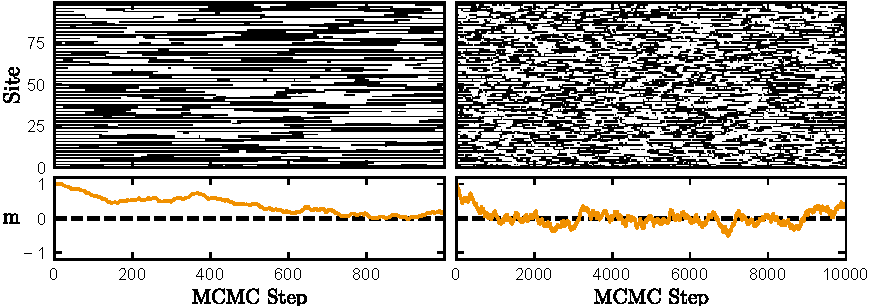
\includegraphics[width=\columnwidth]{pdf_figs/raw_steps_single_flip.pdf}
  \caption{An MCMC walk starting from the staggered charge density wave ground state for a system with $N = 100$ sites and 10,000 MCMC steps. In this simulation only a single spin can be flipped per step according to the Metropolis-Hastings Algorithm. The staggered magnetisation $m = N^{-1} \sum_i (-1)^i \; S_i$ order parameter is plotted below. At this temperature the thermal average of m is zero, while the initial state has m = 1. We see that it takes about 1000 steps for the system to converge, after which it moves about the m = 0 average with a finite auto-correlation time.  $t = 1, \alpha = 1.25, T = 3, J = U = 5 $ \label{fig:raw}}
\end{figure}

\ac{MCMC} sidesteps these issues by defining a random walk that focuses on the states with the greatest Boltzmann weight. At low temperatures this means we need only visit a few low energy states to make good estimates while at high temperatures the weights become uniform so a small number of samples distributed across the state space suffice. However we will see that the method is not without difficulties of its own.

\begin{figure}
  \centering
  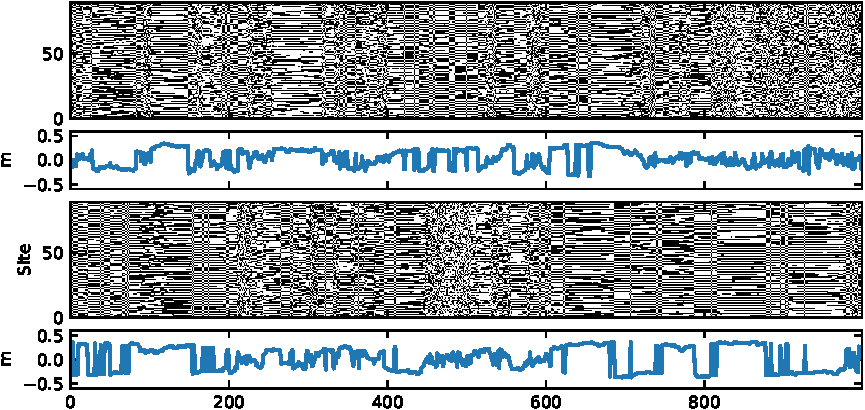
\includegraphics[width=\columnwidth]{pdf_figs/single.pdf}
  \caption{Two MCMC chains starting from the same initial state for a system with $N = 90$ sites and 1000 MCMC steps.  In this simulation the MCMC step is defined differently: an attempt is made to flip n spins, where n is drawn from Uniform(1,N). This is repeated $N^2/100$ times for each step. This trades off computation time for storage space, as it makes the samples less correlated, giving smaller statistical error for a given number of stored samples. These simulations therefore have the potential to necessitate $N^2/100$ matrix diagonalisations for every MCMC sample, though this can be cut down with caching and other tricks. $t = 1, \alpha = 1.25, T = 2.2, J = U = 5 $ \label{fig:single}}
\end{figure}

\%MCMC from an ensemble point of view In implementation \ac{MCMC} can be boiled down to choosing a transition function \$\T(\s\_\{t\} \rightarrow \s\_t+1) \$ where \(\s\) are vectors representing classical spin configurations. We start in some initial state \(\s_0\) and then repeatedly jump to new states according to the probabilities given by \(\T\). This defines a set of random walks \(\{\s_0\ldots \s_i\ldots \s_N\}\). Fig.\textasciitilde{}\ref{fig:single} shows this in practice: we have a (rather small) ensemble of \(M = 2\) walkers starting at the same point in state space and then spreading outwards by flipping spins along the way.

In pseudo-code one could write the MCMC simulation for a single walker as:

\begin{lstlisting}[language=Python]
current_state = initial_state

for i in range(N_steps):
    new_state = sample_T(current_state) 
    states[i] = current_state
\end{lstlisting}

Where the \texttt{sample\_T} function here produces a state with probability determined by the \texttt{current\_state} and the transition function \(\T\).

If we ran many such walkers in parallel we could then approximate the distribution \(p_t(\s; \s_0)\) which tells us where the walkers are likely to be after they've evolved for \(t\) steps from an initial state \(\s_0\). We need to carefully choose \(\T\) such that after a large number of steps \(k\) (the convergence time) the probability \(p_t(\s;\s_0)\) approaches the thermal distribution \(P(\s; \beta) = \Z^{-1} e^{-\beta F(\s)}\). This turns out to be quite easy to achieve using the Metropolis-Hasting algorithm.

\hypertarget{convergence-time}{%
\subsubsection{Convergence Time\}}\label{convergence-time}}

Considering \(p(\s)\) as a vector \(\vec{p}\) whose jth entry is the probability of the jth state \(p_j = p(\s_j)\), and writing \(\T\) as the matrix with entries \(T_{ij} = \T(\s_j \rightarrow \s_i)\) we can write the update rule for the ensemble probability as: \[\vec{p}_{t+1} = \T \vec{p}_t \implies \vec{p}_{t} = \T^t \vec{p}_0\] where \(\vec{p}_0\) is vector which is one on the starting state and zero everywhere else. Since all states must transition to somewhere with probability one: \(\sum_i T_{ij} = 1\).

Matrices that satisfy this are called stochastic matrices exactly because they model these kinds of Markov processes. It can be shown that they have real eigenvalues, and ordering them by magnitude, that \(\lambda_0 = 1\) and \(0 < \lambda_{i\neq0} < 1\). \%https://en.wikipedia.org/wiki/Stochastic\_matrix Assuming \(\T\) has been chosen correctly, its single eigenvector with eigenvalue 1 will be the thermal distribution \footnote{or, in the general case, any desired distribution. MCMC has found a lot of use in sampling from the complicated distributions that arise when taking a Bayesian approach to statistics.} so repeated application of the transition function eventually leads there, while memory of the initial conditions decays exponentially with a convergence time \(k\) determined by \(\lambda_1\). In practice this means that one throws away the data from the beginning of the random walk in order reduce the dependence on the initial conditions and be close enough to the target distribution.

\hypertarget{auto-correlation-time}{%
\subsubsection{Auto-correlation Time\}}\label{auto-correlation-time}}

\begin{figure}
  \centering
  \includegraphics[width=\columnwidth]{figs/m_autocorr.png}
  \caption{(Upper) 10 MCMC chains starting from the same initial state for a system with $N = 150$ sites and 3000 MCMC steps. At each MCMC step, n spins are flipped where n is drawn from Uniform(1,N) and this is repeated $N^2/100$ times. The simulations therefore have the potential to necessitate $10*N^2$ matrix diagonalisations for each 100 MCMC steps. (Lower) The normalised auto-correlation $(\expval{m_i m_{i-j}} - \expval{m_i}\expval{m_i}) / Var(m_i))$ averaged over $i$. It can be seen that even with each MCMC step already being composed of many individual flip attempts, the auto-correlation is still non negligible and must be taken into account in the statistics. $t = 1, \alpha = 1.25, T = 2.2, J = U = 5 $ \label{fig:m_autocorr}}
\end{figure}

At this stage one might think we're done. We can indeed draw independent samples from \(P(\s; \beta)\) by starting from some arbitrary initial state and doing \(k\) steps to arrive at a sample. However a key insight is that after the convergence time, every state generated is a sample from \(P(\s; \beta)\)! They are not, however, independent samples. In Fig.\textasciitilde{}\ref{fig:raw} it is already clear that the samples of the order parameter m have some auto-correlation because only a few spins are flipped each step but even when the number of spins flipped per step is increased, Fig.\textasciitilde{}\ref{fig:m_autocorr} shows that it can be an important effect near the phase transition. Let's define the auto-correlation time \(\tau(O)\) informally as the number of MCMC samples of some observable O that are statistically equal to one independent sample.\textasciitilde{}\footnote{or equivalently as the number of MCMC steps after which the samples are correlated below some cutoff, see~@krauthIntroductionMonteCarlo1996} for a more rigorous definition involving a sum over the auto-correlation function.\} The auto-correlation time is generally shorter than the convergence time so it therefore makes sense from an efficiency standpoint to run a single walker for many MCMC steps rather than to run a huge ensemble for \(k\) steps each.

Once the random walk has been carried out for many steps, the expectation values of \(O\) can be estimated from the MCMC samples \(\s_i\): \[
    \tex{O} = \sum_{i = 0}^{N} O(\s_i) + \mathcal{O}(\frac{1}{\sqrt{N}})
\] The the samples are correlated so the N of them effectively contains less information than \(N\) independent samples would, in fact roughly \(N/\tau\) effective samples. As a consequence the variance is larger than the \(\qex{O^2} - \qex{O}^2\) form it would have if the estimates were uncorrelated. There are many methods in the literature for estimating the true variance of \(\qex{O}\) and deciding how many steps are needed but my approach has been to run a small number of parallel chains, which are independent, in order to estimate the statistical error produced. This is a slightly less computationally efficient because it requires throwing away those \(k\) steps generated before convergence multiple times but it is a conceptually simple workaround.

In summary, to do efficient simulations we want to reduce both the convergence time and the auto-correlation time as much as possible. In order to explain how, we need to introduce the Metropolis-Hasting (MH) algorithm and how it gives an explicit form for the transition function.

\hypertarget{the-metropolis-hastings-algorithm}{%
\subsubsection{The Metropolis-Hastings Algorithm\}}\label{the-metropolis-hastings-algorithm}}

MH breaks up the transition function into a proposal distribution \(q(\s \to \s')\) and an acceptance function \(\A(\s \to \s')\). \(q\) needs to be something that we can directly sample from, and in our case generally takes the form of flipping some number of spins in \(\s\), i.e if we're flipping a single random spin in the spin chain, \(q(\s \to \s')\) is the uniform distribution on states reachable by one spin flip from \(\s\). This also gives the nice symmetry property that \(q(\s \to \s') = q(\s' \to \s)\).

The proposal \(\s'\) is then accepted or rejected with an acceptance probability \(\A(\s \to \s')\), if the proposal is rejected then \(\s_{i+1} = \s_{i}\). Hence:

\[\T(x\to x') = q(x\to x')\A(x \to x')\]

When the proposal distribution is symmetric as ours is, it cancels out in the expression for the acceptance function and the Metropolis-Hastings algorithm is simply the choice: \[ \A(x \to x') = \min\left(1, e^{-\beta\;\Delta F}\right)\] Where \(F\) is the overall free energy of the system, including both the quantum and classical sector.

To implement the acceptance function in practice we pick a random number in the unit interval and accept if it is less than \(e^{-\beta\;\Delta F}\):

\begin{lstlisting}[language=Python]
current_state = initial_state

for i in range(N_steps):
    new_state = proposal(current_state)
    df = free_energy_change(current_state, new_state, parameters)

    if uniform(0,1) < exp(-beta * df):
        current_state = new_state
        
    states[i] = current_state
\end{lstlisting}

This has the effect of always accepting proposed states that are lower in energy and sometimes accepting those that are higher in energy than the current state.

\hypertarget{choosing-the-proposal-distribution}{%
\subsubsection{Choosing the proposal distribution\}}\label{choosing-the-proposal-distribution}}

\begin{figure}[H]
  \centering
  \includegraphics[width=\columnwidth]{figs/autocorr_multiple_proposals.png}
  Simulations showing how the autocorrelation of the order parameter depends on the proposal distribution used at different temperatures, we see that at $T = 1.5 < T_c$ a single spin flip is likely the best choice, while at the high temperature $T = 2.5 > T_c$ flipping two sites or a mixture of flipping two and 1 sites is likely a better choice. 
  \caption{ $t = 1, \alpha = 1.25, J = U = 5 $ \label{fig:comparison}}
\end{figure}

Now we can discuss how to minimise the auto-correlations. The general principle is that one must balance the proposal distribution between two extremes. Choose overlay small steps, like flipping only a single spin and the acceptance rate will be high because \(\Delta F\) will usually be small, but each state will be very similar to the previous and the auto-correlations will be high too, making sampling inefficient. On the other hand, overlay large steps, like randomising a large portion of the spins each step, will result in very frequent rejections, especially at low temperatures.

I evaluated a few different proposal distributions for use with the FK model.

\begin{enumerate}
\item Flipping a single random site
\item Flipping N random sites for some N
\item Choosing n from Uniform(1, N) and then flipping n sites for some fixed N.
\item Attempting to tune the proposal distribution for each parameter regime.
\end{enumerate}

Fro Figure\textasciitilde{}\ref{fig:comparison} we see that even at moderately high temperatures \(T > T_c\) flipping one or two sites is the best choice. However for some simulations at very high temperature flipping more spins is warranted. Tuning the proposal distribution automatically seems like something that would not yield enough benefit for the additional complexity it would require.

\hypertarget{two-step-trick}{%
\subsubsection{Two Step Trick}\label{two-step-trick}}

Our method already relies heavily on the split between the classical and quantum sector to derive a sign problem free MCMC algorithm but it turns out that there is a further trick we can play with it. The free energy term is the sum of an easy to compute classical energy and a more expensive quantum free energy, we can split the acceptance function into two in such as way as to avoid having to compute the full exact diagonalisation some of the time:

\begin{Shaded}
\begin{Highlighting}[]

\NormalTok{current\_state }\OperatorTok{=}\NormalTok{ initial\_state}

\ControlFlowTok{for}\NormalTok{ i }\KeywordTok{in} \BuiltInTok{range}\NormalTok{(N\_steps):}
\NormalTok{    new\_state }\OperatorTok{=}\NormalTok{ proposal(current\_state)}

\NormalTok{    df\_classical }\OperatorTok{=}\NormalTok{ classical\_free\_energy\_change(current\_state, new\_state, parameters)}
    \ControlFlowTok{if}\NormalTok{ exp(}\OperatorTok{{-}}\NormalTok{beta }\OperatorTok{*}\NormalTok{ df\_classical) }\OperatorTok{\textless{}}\NormalTok{ uniform(}\DecValTok{0}\NormalTok{,}\DecValTok{1}\NormalTok{):}
\NormalTok{        f\_quantum }\OperatorTok{=}\NormalTok{ quantum\_free\_energy(current\_state, new\_state, parameters)}
    
        \ControlFlowTok{if}\NormalTok{ exp(}\OperatorTok{{-}}\NormalTok{ beta }\OperatorTok{*}\NormalTok{ df\_quantum) }\OperatorTok{\textless{}}\NormalTok{ uniform(}\DecValTok{0}\NormalTok{,}\DecValTok{1}\NormalTok{):}
\NormalTok{          current\_state }\OperatorTok{=}\NormalTok{ new\_state}
    
\NormalTok{        states[i] }\OperatorTok{=}\NormalTok{ current\_state}
    
\end{Highlighting}
\end{Shaded}

lets cite Figure \ref{fig:binder}

lets cite to person \textcite{trebstKitaevMaterials2022}. and then multple \autocite{banerjeeProximateKitaevQuantum2016,trebstKitaevMaterials2022}. what is we surround it by spaces? \textcite{trebstKitaevMaterials2022}

\begin{Shaded}
\begin{Highlighting}[]

\end{Highlighting}
\end{Shaded}

\begin{Shaded}
\begin{Highlighting}[]

\end{Highlighting}
\end{Shaded}

% \hypertarget{markov-chain-monte-carlo}{%
\section{Markov Chain Monte Carlo}\label{markov-chain-monte-carlo}}

\hypertarget{sampling}{%
\subsection{Sampling}\label{sampling}}

Markov Chain Monte Carlo (MCMC) is a useful method whenever we have a probability distribution that we want to sample from but there is not direct sampling way to do so.

In almost any computer simulation the ultimate source of randomness is a stream of (close to) uniform, uncorrelated bits generated from a pseudo random number generator. A direct sampling method takes such a source and outputs uncorrelated samples from the target distribution. The fact they're uncorrelated is key as we'll see later. Examples of direct sampling methods range from the trivial: take n random bits to generate integers uniformly between 0 and \(2^n\) to more complex methods such as inverse transform sampling and rejection sampling \autocite{devroyeRandomSampling1986}.

In physics the distribution we usually want to sample from is the Boltzmann probability over states of the system \(S\): \[
\begin{aligned}
p(S)  &= \frac{1}{\mathcal{Z}} e^{-\beta H(S)} \\
\end{aligned}
\] where \(\mathcal{Z} = \sum_S e^{-\beta H(S)}\) is the normalisation factor and ubiquitous partition function. In principle we could directly sample from this, for a discrete system there are finitely many choices. We could calculate the probability of each one and assign each a region of the unit interval which we could then sample uniformly from.

However if we actually try to do this we will run into two problems, we can't calculate \(\mathcal{Z}\) for any reasonably sized systems because the state space grows exponentially with system size. Even if we could calculate \(\mathcal{Z}\), sampling from an exponentially large number of options quickly become tricky. This kind of problem happens in many other disciplines too, particularly when fitting statistical models using Bayesian inference \autocite{BMCP2021}.

\hypertarget{markov-chains}{%
\subsection{Markov Chains}\label{markov-chains}}

So what can we do? Well it turns out that if we're willing to give up in the requirement that the samples be uncorrelated then we can use MCMC instead.

MCMC defines a weighted random walk over the states \((S_0, S_1, S_2, ...)\), such that in the long time limit, states are visited according to their probability \(p(S)\). \autocite{binderGuidePracticalWork1988,kerteszAdvancesComputerSimulation1998,wolffMonteCarloErrors2004}.

In a physics context this lets us evaluate any observable with a mean over the states visited by the walk. \[\begin{aligned}
\langle O \rangle & = \sum_{S} p(S) \langle O \rangle_{S} = \sum_{i = 0}^{M} \expval{O}_{S_i} + \mathcal{O}(\tfrac{1}{\sqrt{M}})\\
\end{aligned}\]

The choice of the transition function for MCMC is under-determined as one only needs to satisfy a set of balance conditions for which there are many solutions~\autocite{kellyReversibilityStochasticNetworks1981}.

\hypertarget{application-to-the-fk-model}{%
\subsection{Application to the FK Model}\label{application-to-the-fk-model}}

We will work in the grand canonical ensemble of fixed temperature, chemical potential and volume.

Since the spin configurations are classical, the Hamiltonian can be split into a classical spin part \(H_s\) and an operator valued part \(H_c\). \[\begin{aligned}
H_s& = - \frac{U}{2}S_i + \sum_{i, j}^{N} J_{ij} S_i S_j \\
H_c& = \sum_i U S_i c^\dagger_{i}c_{i} -t(c^\dagger_{i}c_{i+1} + c^\dagger_{i+1}c_{i}) 
\end{aligned}\] The partition function can then be written as a sum over spin configurations, \(\vec{S} = (S_0, S_1...S_{N-1})\): \[\begin{aligned}
\mathcal{Z} = \mathrm{Tr} e^{-\beta H}= \sum_{\vec{S}} e^{-\beta H_s} \mathrm{Tr}_c e^{-\beta H_c} .
\end{aligned}
\] The contribution of \(H_c\) to the grand canonical partition function can be obtained by performing the sum over eigenstate occupation numbers giving \(-\beta F_c[\vec{S}] = \sum_k \ln{(1 + e^{- \beta \epsilon_k})}\) where \({\epsilon_k[\vec{S}]}\) are the eigenvalues of the matrix representation of \(H_c\) determined through exact diagonalisation. This gives a partition function containing a classical energy which corresponds to the long-range interaction of the spins, and a free energy which corresponds to the quantum subsystem. \[\begin{aligned}
\mathcal{Z} = \sum_{\vec{S}} e^{-\beta H_S[\vec{S}] - \beta F_c[\vec{S}]} = \sum_{\vec{S}} e^{-\beta E[\vec{S}]}
\end{aligned}\]

\hypertarget{markov-chain-monte-carlo-1}{%
\subsubsection{Markov Chain Monte Carlo}\label{markov-chain-monte-carlo-1}}

Markov Chain Monte Carlo (MCMC) is a technique for evaluating thermal expectation values \(\expval{O}\) with respect to some physical system defined by a set of states \(\{x: x \in S\}\) and a free energy \(F(x)\) \autocite{krauthIntroductionMonteCarlo1998}. The thermal expectation value is defined via a Boltzmann weighted sum over the entire states: \[
\begin{aligned}
    \expval{O} &= \frac{1}{\mathcal{Z}} \sum_{x \in S} O(x) P(x) \\
    P(x) &= \frac{1}{\mathcal{Z}} e^{-\beta F(x)} \\
    \mathcal{Z} &= \sum_{x \in S} e^{-\beta F(x)}
\end{aligned}
\]

When the state space is too large to evaluate this sum directly, MCMC defines a stochastic algorithm which generates a random walk \(\{x_0\ldots x_i\ldots x_N\}\) whose distribution \(p(x_i)\) approaches a target distribution \(P(x)\) in the large N limit.

\[\lim_{i\to\infty} p(x_i) = P(x)\]

In this case the target distribution will be the thermal one \(P(x) \rightarrow \mathcal{Z}^{-1} e^{-\beta F(x)}\). The major benefit of the method being that as long as one can express the desired \(P(x)\) up to a multiplicative constant, MCMC can be applied. Since \(e^{-\beta F(x)}\) is relatively easy to evaluate, MCMC provides a useful method for finite temperature physics.

Once the random walk has been carried out for many steps, the expectation values of \(O\) can be estimated from the MCMC samples: \[
    \expval{O} = \sum_{i = 0}^{N} O(x_i) + \mathcal{O}(\frac{1}{\sqrt{N}})
\] The the samples in the random walk are correlated so the samples effectively contain less information than \(N\) independent samples would. As a consequence the variance is larger than the \(\expval{O^2} - \expval{O}^2\) form it would have if the estimates were uncorrelated. Methods of estimating the true variance of \(\expval{O}\) and decided how many steps are needed will be considered later.

\hypertarget{the-metropolis-hasting-algorithm}{%
\subsection{The Metropolis-Hasting Algorithm}\label{the-metropolis-hasting-algorithm}}

Markov chains are defined by a transition function \$\mathcal{T}(x\_\{i+1\} \rightarrow x\_i) \$ giving the probability that a chain in state \(x_i\) at time \(i\) will transition to a state \(x_{i+1}\). Since we must transition somewhere at each step, this comes with the normalisation condition that \(\sum\limits_x \mathcal{T}(x' \rightarrow x) = 1\).

If we define an ensemble of Markov chains and consider the distributions we get a sequence of distributions \(\{p_0(x), p_1(x), p_2(x)\ldots\}\) with \[\begin{aligned}
p_{i+1}(x) &= \sum_{x' \in S} p_i(x') \mathcal{T}(x' \rightarrow x)
\end{aligned}\] \(p_o(x)\) might be a delta function on one particular starting state which would then be smoothed out by the transition function repeatedly.

As we'd like to draw samples from the target distribution \(P(x)\) the trick is to choose \$\mathcal{T}(x\_\{i+1\} \rightarrow x\_i) \$ such that :

\[\begin{aligned}
P(x) &= \sum_{x'} P(x') \mathcal{T}(x' \rightarrow x)
\end{aligned}
\] In other words the MCMC dynamics defined by \(\mathcal{T}\) must be constructed to have the target distribution as their only fixed point. This condition is called the global balance condition. Along with some more technical considerations such as ergodicity which won't be considered here, global balance suffices to ensure that a MCMC method is correct.

A sufficient but not necessary condition for global balance to hold is detailed balance:

\[
P(x) \mathcal{T}(x \rightarrow x') = P(x') \mathcal{T}(x' \rightarrow x)
\] \% In practice most algorithms are constructed to satisfy detailed balance though there are arguments that relaxing the condition can lead to faster algorithms \autocite{kapferSamplingPolytopeHarddisk2013}.

The goal of MCMC is then to choose \(\mathcal{T}\) so that it has the desired thermal distribution \(P(x)\) as its fixed point and that it converges quickly onto it. This boils down to requiring that the matrix representation of \(T_{ij} = \mathcal{T}(x_i \to x_j)\) has an eigenvector equal to \(P_i = P(x_i)\) with eigenvalue 1 and all other eigenvalues with magnitude less than one. The convergence time depends on the magnitude of the second largest eigenvalue.

\hypertarget{metropolis-hastings}{%
\subsection{Metropolis-Hastings}\label{metropolis-hastings}}

In order to actually choose new states according to \(\mathcal{T}\) one chooses states from a proposal distribution \(q(x_i \to x')\) that can be directly sampled from. For instance, this might mean flipping a single random spin in a spin chain, in which case \(q(x'\to x_i)\) is the uniform distribution on states reachable by one spin flip from \(x_i\). The proposal \(x'\) is then accepted or rejected with an acceptance probability \(\mathcal{A}(x'\to x_{i+1})\), if the proposal is rejected then \(x_{i+1} = x_{i}\). Now \(\mathcal{T}(x\to x') = q(x\to x')\mathcal{A}(x \to x')\).

The Metropolis-Hasting algorithm is a slight extension of the original Metropolis algorithm that allows for non-symmetric proposal distributions \$q(x\to x') \neq q(x'\to x) \$. It can be derived starting from detailed balance \autocite{krauthIntroductionMonteCarlo1998}: \[\begin{aligned}
P(x)\mathcal{T}(x \to x') &= P(x')\mathcal{T}(x' \to x) \\
P(x)q(x \to x')\mathcal{A}(x \to x') &= P(x')q(x' \to x)\mathcal{A}(x' \to x) \\
\label{eq:db2} \frac{\mathcal{A}(x \to x')}{\mathcal{A}(x' \to x)} &= \frac{P(x')q(x' \to x)}{P(x)q(x \to x')} = f(x, x')\\
\end{aligned}
\] \% The Metropolis-Hastings algorithm is the choice: \[
\begin{aligned}
\label{eq:mh} 
\mathcal{A}(x \to x') = \min\left(1, f(x,x')\right)
\end{aligned}
\] \% Noting that \(f(x,x') = 1/f(x',x)\), Eq. \ref{eq:mh} can be seen to satisfy Eq. \ref{eq:db2} by considering the two cases \(f(x,x') > 1\) and \(f(x,x') < 1\).

By choosing the proposal distribution such that \(f(x,x')\) is as close as possible to one, the rate of rejections can be reduced and the algorithm sped up.

\hypertarget{convergence-auto-correlation-and-binning}{%
\subsection{Convergence, Auto-correlation and Binning}\label{convergence-auto-correlation-and-binning}}

\%Thinning, burn in, multiple runs

\hypertarget{applying-mcmc-to-the-fk-model}{%
\section{Applying MCMC to the FK model}\label{applying-mcmc-to-the-fk-model}}

MCMC can be applied to sample over the classical degrees of freedom of the model. We take the full Hamiltonian and split it into a classical and a quantum part: \[\begin{aligned}
    H_{\mathrm{FK}} &= -\sum_{<ij>} c^\dagger_{i}c_{j} + U \sum_{i} (c^\dagger_{i}c_{i} - 1/2)( n_i - 1/2) \\
    &+ \sum_{ij} J_{ij} (n_i - 1/2) (n_j - 1/2)  - \mu \sum_i (c^\dagger_{i}c_{i} + n_i)\\
    H_q &= -\sum_{<ij>} c^\dagger_{i}c_{j} + \sum_{i} \left(U(n_i - 1/2) - \mu\right) c^\dagger_{i}c_{i}\\
    H_c &= \sum_i \mu n_i - \frac{U}{2}(n_i - 1/2) + \sum_{ij}J_{ij}(n_i - 1/2)(n_j - 1/2)
\end{aligned}
\] \% There are \(2^N\) possible ion configurations \(\{ n_i \}\), we define \(n^k_i\) to be the occupation of the ith site of the kth configuration. The quantum part of the free energy can then be defined through the quantum partition function \(\mathcal{Z}^k\) associated with each ionic state \(n^k_i\): \[\begin{aligned}
F^k &= -1/\beta \ln{\mathcal{Z}^k} \\
\end{aligned}\] \% Such that the overall partition function is: \[\begin{aligned}
\mathcal{Z} &= \sum_k e^{- \beta H^k} Z^k \\
&= \sum_k e^{-\beta (H^k + F^k)} \\
\end{aligned}\] \% Because fermions are limited to occupation numbers of 0 or 1 \(Z^k\) simplifies nicely. If \(m^j_i = \{0,1\}\) is defined as the occupation of the level with energy \(\epsilon^k_i\) then the partition function is a sum over all the occupation states labelled by j: \[\begin{aligned}
Z^k    &= \Tr e^{-\beta F^k} = \sum_j e^{-\beta \sum_i m^j_i \epsilon^k_i}\\
       &= \sum_j \prod_i e^{- \beta m^j_i \epsilon^k_i}= \prod_i \sum_j e^{- \beta m^j_i \epsilon^k_i}\\
       &= \prod_i (1 + e^{- \beta \epsilon^k_i})\\
F^k    &= -1/\beta \sum_k \ln{(1 + e^{- \beta \epsilon^k_i})}
\end{aligned}\] \% Observables can then be calculated from the partition function, for examples the occupation numbers:

\[\begin{aligned}
\tex{N} &= \frac{1}{\beta} \frac{1}{Z} \frac{\partial Z}{\partial \mu} = - \frac{\partial F}{\partial \mu}\\
    &= \frac{1}{\beta} \frac{1}{Z} \frac{\partial}{\partial \mu} \sum_k e^{-\beta (H^k + F^k)}\\
    &= 1/Z \sum_k (N^k_{\mathrm{ion}} + N^k_{\mathrm{electron}}) e^{-\beta (H^k + F^k)}\\
\end{aligned}\] \% with the definitions:

\[\begin{aligned}
N^k_{\mathrm{ion}} &= - \frac{\partial H^k}{\partial \mu} = \sum_i n^k_i\\
N^k_{\mathrm{electron}} &= - \frac{\partial F^k}{\partial \mu} = \sum_i \left(1 + e^{\beta \epsilon^k_i}\right)^{-1}\\
\end{aligned}\] \% The MCMC algorithm consists of performing a random walk over the states \(\{ n^k_i \}\). In the simplest case the proposal distribution corresponds to flipping a random site from occupied to unoccupied or vice versa, since this proposal is symmetric the acceptance function becomes: \[\begin{aligned} 
P(k) &= \mathcal{Z}^{-1} e^{-\beta(H^k + F^k)} \\
\mathcal{A}(k \to k') &= \min\left(1, \frac{P(k')}{P(k)}\right) = \min\left(1, e^{\beta(H^{k'} + F^{k'})-\beta(H^k + F^k)}\right)
\end{aligned}\] \% At each step \(F^k\) is calculated by diagonalising the tri-diagonal matrix representation of \(H_q\) with open boundary conditions. Observables are simply averages over the their value at each step of the random walk. The full spectrum and eigenbasis is too large to save to disk so usually running averages of key observables are taken as the walk progresses.

\hypertarget{proposal-distributions}{%
\subsection{Proposal Distributions}\label{proposal-distributions}}

In a MCMC method a key property is the proportion of the time that proposals are accepted, the acceptance rate. If this rate is too low the random walk is trying to take overly large steps in energy space which problematic because it means very few new samples will be generated. If it is too high it implies the steps are too small, a problem because then the walk will take longer to explore the state space and the samples will be highly correlated. Ideal values for the acceptance rate can be calculated under certain assumptions \autocite{robertsWeakConvergenceOptimal1997}. Here we monitor the acceptance rate and if it is too high we re-run the MCMC with a modified proposal distribution that has a chance to propose moves that flip multiple sites at a time.

In addition we exploit the particle-hole symmetry of the problem by occasionally proposing a flip of the entire state. This works because near half-filling, flipping the occupations of all the sites will produce a state at or near the energy of the current one.

\hypertarget{perturbation-mcmc}{%
\subsection{Perturbation MCMC}\label{perturbation-mcmc}}

The matrix diagonalisation is the most computationally expensive step of the process, a speed up can be obtained by modifying the proposal distribution to depend on the classical part of the energy, a trick gleaned from Ref. \autocite{krauthIntroductionMonteCarlo1998}: \[
\begin{aligned}
q(k \to k') &= \min\left(1, e^{\beta (H^{k'} - H^k)}\right) \\
\mathcal{A}(k \to k') &= \min\left(1, e^{\beta(F^{k'}- F^k)}\right)
\end{aligned}\] \% This allows the method to reject some states without performing the diagonalisation at no cost to the accuracy of the MCMC method.

An extension of this idea is to try to define a classical model with a similar free energy dependence on the classical state as the full quantum, Ref. \autocite{huangAcceleratedMonteCarlo2017} does this with restricted Boltzmann machines whose form is very similar to a classical spin model.

\hypertarget{scaling}{%
\subsection{Scaling}\label{scaling}}

In order to reduce the effects of the boundary conditions and the finite size of the system we redefine and normalise the coupling matrix to have 0 derivative at its furthest extent rather than cutting off abruptly.

\[
\begin{aligned}
J'(x) &= \abs{\frac{L}{\pi}\sin \frac{\pi x}{L}}^{-\alpha} \\
J(x) &= \frac{J_0 J'(x)}{\sum_y J'(y)}
\end{aligned}\] \% The scaling ensures that, in the ordered phase, the overall potential felt by each site due to the rest of the system is independent of system size.

\hypertarget{binder-cumulants}{%
\subsection{Binder Cumulants}\label{binder-cumulants}}

The Binder cumulant is defined as: \[U_B = 1 - \frac{\tex{\mu_4}}{3\tex{\mu_2}^2}\] \% where \[\mu_n = \tex{(m - \tex{m})^n}\] \% are the central moments of the order parameter m: \[m = \sum_i (-1)^i (2n_i - 1) / N\] \% The Binder cumulant evaluated against temperature can be used as a diagnostic for the existence of a phase transition. If multiple such curves are plotted for different system sizes, a crossing indicates the location of a critical point \autocite{binderFiniteSizeScaling1981,musialMonteCarloSimulations2002}.

\hypertarget{markov-chain-monte-carlo-in-practice}{%
\subsection{Markov Chain Monte-Carlo in Practice}\label{markov-chain-monte-carlo-in-practice}}

\hypertarget{quick-intro-to-mcmc}{%
\subsubsection{Quick Intro to MCMC}\label{quick-intro-to-mcmc}}

The main paper relies on \ac{MCMC} extensively to evaluate thermal expectation values within the \ac{FK} model by walking over states of the classical spin system \(S_i\). For a classical system, the thermal expectation value of some operator \(O\) is defined by a Boltzmann weighted sum over the classical state space: \[\being{aligned}
    \tex{O} &= \frac{1}{\mathcal{Z}} \sum_{\s \in S} O(x) P(x) \\
    P(x) &= \frac{1}{\mathcal{Z}} e^{-\beta F(x)} \\
    \mathcal{Z} &= \sum_{\s \in S} e^{-\beta F(x)}
\end{aligned}\] While for a quantum system these sums are replaced by equivalent traces. The obvious approach to evaluate these sums numerically would be to directly loop over all the classical states in the system and perform the sum. But we all know know why this isn't feasible: the state space is too large! Indeed even if we could do it, it would still be computationally wasteful since at low temperatures the sums are dominated by low energy excitations about the ground states of the system. Even worse, in our case we must fully solve the fermionic system via exact diagonalisation for each classical state in the sum, a very expensive operation!\textasciitilde\textbackslash footnote\{The effort involved in exact diagonalisation scales like \(N^2\) for systems with a tri-diagonal matrix representation (open boundary conditions and nearest neighbour hopping) and like \(N^3\) for a generic matrix \autocite{bolchQueueingNetworksMarkov2006,usmaniInversionTridiagonalJacobi1994}.

c

MCMC sidesteps these issues by defining a random walk that focuses on the states with the greatest Boltzmann weight. At low temperatures this means we need only visit a few low energy states to make good estimates while at high temperatures the weights become uniform so a small number of samples distributed across the state space suffice. However we will see that the method is not without difficulties of its own.

\begin{figure}
  \centering
  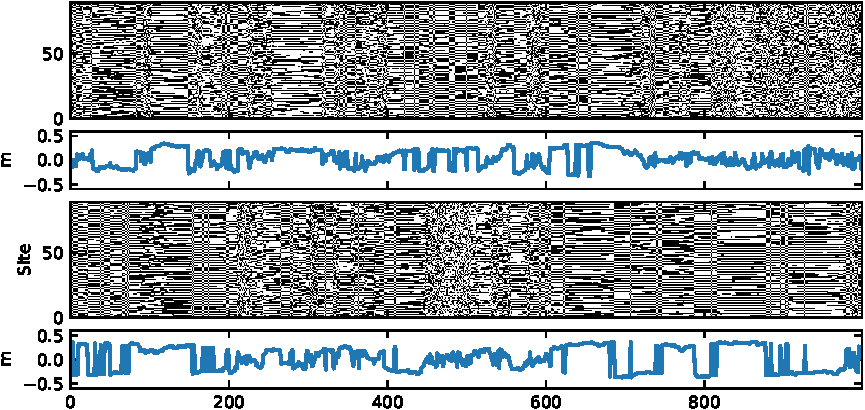
\includegraphics[width=\columnwidth]{pdf_figs/single.pdf}
  \caption{Two MCMC chains starting from the same initial state for a system with $N = 90$ sites and 1000 MCMC steps.  In this simulation the MCMC step is defined differently: an attempt is made to flip n spins, where n is drawn from Uniform(1,N). This is repeated $N^2/100$ times for each step. This trades off computation time for storage space, as it makes the samples less correlated, giving smaller statistical error for a given number of stored samples. These simulations therefore have the potential to necessitate $N^2/100$ matrix diagonalisations for every MCMC sample, though this can be cut down with caching and other tricks. $t = 1, \alpha = 1.25, T = 2.2, J = U = 5 $ \label{fig:single}}
\end{figure}

\%MCMC from an ensemble point of view In implementation \ac{MCMC} can be boiled down to choosing a transition function \$\mathcal{T}(\s\_\{t\} \rightarrow \s\_t+1) \$ where \(\s\) are vectors representing classical spin configurations. We start in some initial state \(\s_0\) and then repeatedly jump to new states according to the probabilities given by \(\mathcal{T}\). This defines a set of random walks \(\{\s_0\ldots \s_i\ldots \s_N\}\). Fig.\textasciitilde{}\ref{fig:single} shows this in practice: we have a (rather small) ensemble of \(M = 2\) walkers starting at the same point in state space and then spreading outwards by flipping spins along the way.

In pseudo-code one could write the MCMC simulation for a single walker as:

\begin{Shaded}
\begin{Highlighting}[]
\NormalTok{current\_state }\OperatorTok{=}\NormalTok{ initial\_state}

\ControlFlowTok{for}\NormalTok{ i }\KeywordTok{in} \BuiltInTok{range}\NormalTok{(N\_steps):}
\NormalTok{    new\_state }\OperatorTok{=}\NormalTok{ sample\_T(current\_state) }
\NormalTok{    states[i] }\OperatorTok{=}\NormalTok{ current\_state}
\end{Highlighting}
\end{Shaded}

Where the \texttt{sample\_T} function here produces a state with probability determined by the \texttt{current\_state} and the transition function \(\mathcal{T}\).

If we ran many such walkers in parallel we could then approximate the distribution \(p_t(\s; \s_0)\) which tells us where the walkers are likely to be after they've evolved for \(t\) steps from an initial state \(\s_0\). We need to carefully choose \(\mathcal{T}\) such that after a large number of steps \(k\) (the convergence time) the probability \(p_t(\s;\s_0)\) approaches the thermal distribution \(P(\s; \beta) = \mathcal{Z}^{-1} e^{-\beta F(\s)}\). This turns out to be quite easy to achieve using the Metropolis-Hasting algorithm.

\hypertarget{convergence-time}{%
\subsubsection{Convergence Time}\label{convergence-time}}

Considering \(p(\s)\) as a vector \(\vec{p}\) whose jth entry is the probability of the jth state \(p_j = p(\s_j)\), and writing \(\mathcal{T}\) as the matrix with entries \(T_{ij} = \mathcal{T}(\s_j \rightarrow \s_i)\) we can write the update rule for the ensemble probability as: \[\vec{p}_{t+1} = \mathcal{T} \vec{p}_t \implies \vec{p}_{t} = \mathcal{T}^t \vec{p}_0\] where \(\vec{p}_0\) is vector which is one on the starting state and zero everywhere else. Since all states must transition to somewhere with probability one: \(\sum_i T_{ij} = 1\).

Matrices that satisfy this are called stochastic matrices exactly because they model these kinds of Markov processes. It can be shown that they have real eigenvalues, and ordering them by magnitude, that \(\lambda_0 = 1\) and \(0 < \lambda_{i\neq0} < 1\). \%https://en.wikipedia.org/wiki/Stochastic\_matrix

Assuming \(\mathcal{T}\) has been chosen correctly, its single eigenvector with eigenvalue 1 will be the thermal distribution \footnote{or, in the general case, any desired distribution. MCMC has found a lot of use in sampling from the complicated distributions that arise when taking a Bayesian approach to statistics.} so repeated application of the transition function eventually leads there, while memory of the initial conditions decays exponentially with a convergence time \(k\) determined by \(\lambda_1\). In practice this means that one throws away the data from the beginning of the random walk in order reduce the dependence on the initial conditions and be close enough to the target distribution.

\hypertarget{auto-correlation-time}{%
\subsubsection{Auto-correlation Time}\label{auto-correlation-time}}

\begin{figure}
\hypertarget{fig:m_autocorr}{%
\centering
\includegraphics[width=1\textwidth,height=\textheight]{figure_code/fk_chapter/lsr/figs/m_autocorr.png}
\caption[no title]{(Upper) 10 MCMC chains starting from the same initial state for
a system with \(N = 150\) sites and 3000 MCMC steps. At each MCMC step,
n spins are flipped where n is drawn from Uniform(1,N) and this is
repeated \(N^2/100\) times. The simulations therefore have the potential
to necessitate \(10*N^2\) matrix diagonalisations for each 100 MCMC
steps. (Lower) The normalised auto-correlation
\((\expval{m_i m_{i-j}} - \expval{m_i}\expval{m_i}) / Var(m_i))\)
averaged over \(i\). It can be seen that even with each MCMC step
already being composed of many individual flip attempts, the
auto-correlation is still non negligible and must be taken into account
in the statistics.
\(t = 1, \alpha = 1.25, T = 2.2, J = U = 5\)}\label{fig:m_autocorr}
}
\end{figure}

At this stage one might think we're done. We can indeed draw independent samples from \(P(\s; \beta)\) by starting from some arbitrary initial state and doing \(k\) steps to arrive at a sample. However a key insight is that after the convergence time, every state generated is a sample from \(P(\s; \beta)\)! They are not, however, independent samples. In Fig.\textasciitilde{}\ref{fig:raw} it is already clear that the samples of the order parameter m have some auto-correlation because only a few spins are flipped each step but even when the number of spins flipped per step is increased, Fig.\textasciitilde{}\ref{fig:m_autocorr} shows that it can be an important effect near the phase transition. Let's define the auto-correlation time \(\tau(O)\) informally as the number of MCMC samples of some observable O that are statistically equal to one independent sample or equivalently as the number of MCMC steps after which the samples are correlated below some cutoff, see \autocite{krauthIntroductionMonteCarlo1996} for a more rigorous definition involving a sum over the auto-correlation function. The auto-correlation time is generally shorter than the convergence time so it therefore makes sense from an efficiency standpoint to run a single walker for many MCMC steps rather than to run a huge ensemble for \(k\) steps each.

Once the random walk has been carried out for many steps, the expectation values of \(O\) can be estimated from the MCMC samples \(\s_i\): \[
    \tex{O} = \sum_{i = 0}^{N} O(\s_i) + \mathcal{O}(\frac{1}{\sqrt{N}})
\] The the samples are correlated so the N of them effectively contains less information than \(N\) independent samples would, in fact roughly \(N/\tau\) effective samples. As a consequence the variance is larger than the \(\qex{O^2} - \qex{O}^2\) form it would have if the estimates were uncorrelated. There are many methods in the literature for estimating the true variance of \(\qex{O}\) and deciding how many steps are needed but my approach has been to run a small number of parallel chains, which are independent, in order to estimate the statistical error produced. This is a slightly less computationally efficient because it requires throwing away those \(k\) steps generated before convergence multiple times but it is a conceptually simple workaround.

In summary, to do efficient simulations we want to reduce both the convergence time and the auto-correlation time as much as possible. In order to explain how, we need to introduce the Metropolis-Hasting (MH) algorithm and how it gives an explicit form for the transition function.

\hypertarget{the-metropolis-hastings-algorithm}{%
\subsubsection{The Metropolis-Hastings Algorithm}\label{the-metropolis-hastings-algorithm}}

MH breaks up the transition function into a proposal distribution \(q(\s \to \s')\) and an acceptance function \(\mathcal{A}(\s \to \s')\). \(q\) needs to be something that we can directly sample from, and in our case generally takes the form of flipping some number of spins in \(\s\), i.e if we're flipping a single random spin in the spin chain, \(q(\s \to \s')\) is the uniform distribution on states reachable by one spin flip from \(\s\). This also gives the nice symmetry property that \(q(\s \to \s') = q(\s' \to \s)\).

The proposal \(\s'\) is then accepted or rejected with an acceptance probability \(\mathcal{A}(\s \to \s')\), if the proposal is rejected then \(\s_{i+1} = \s_{i}\). Hence:

\[\mathcal{T}(x\to x') = q(x\to x')\mathcal{A}(x \to x')\]

When the proposal distribution is symmetric as ours is, it cancels out in the expression for the acceptance function and the Metropolis-Hastings algorithm is simply the choice: \[ \mathcal{A}(x \to x') = \min\left(1, e^{-\beta\;\Delta F}\right)\] Where \(F\) is the overall free energy of the system, including both the quantum and classical sector.

To implement the acceptance function in practice we pick a random number in the unit interval and accept if it is less than \(e^{-\beta\;\Delta F}\):

\begin{Shaded}
\begin{Highlighting}[]
\NormalTok{current\_state }\OperatorTok{=}\NormalTok{ initial\_state}

\ControlFlowTok{for}\NormalTok{ i }\KeywordTok{in} \BuiltInTok{range}\NormalTok{(N\_steps):}
\NormalTok{    new\_state }\OperatorTok{=}\NormalTok{ proposal(current\_state)}
\NormalTok{    df }\OperatorTok{=}\NormalTok{ free\_energy\_change(current\_state, new\_state, parameters)}

    \ControlFlowTok{if}\NormalTok{ uniform(}\DecValTok{0}\NormalTok{,}\DecValTok{1}\NormalTok{) }\OperatorTok{\textless{}}\NormalTok{ exp(}\OperatorTok{{-}}\NormalTok{beta }\OperatorTok{*}\NormalTok{ df):}
\NormalTok{        current\_state }\OperatorTok{=}\NormalTok{ new\_state}
        
\NormalTok{    states[i] }\OperatorTok{=}\NormalTok{ current\_state}
\end{Highlighting}
\end{Shaded}

This has the effect of always accepting proposed states that are lower in energy and sometimes accepting those that are higher in energy than the current state.

\hypertarget{two-step-trick}{%
\subsection{Two Step Trick}\label{two-step-trick}}

Here, we incorporate a modification to the standard Metropolis-Hastings algorithm~\autocite{hastingsMonteCarloSampling1970} gleaned from Krauth~\autocite{krauthIntroductionMonteCarlo1998}.

In our computations~\autocite{hodsonMCMCFKModel2021} we employ a modification of the algorithm which is based on the observation that the free energy of the FK system is composed of a classical part which is much quicker to compute than the quantum part. Hence, we can obtain a computational speedup by first considering the value of the classical energy difference \(\Delta H_s\) and rejecting the transition if the former is too high. We only compute the quantum energy difference \(\Delta F_c\) if the transition is accepted. We then perform a second rejection sampling step based upon it. This corresponds to two nested comparisons with the majority of the work only occurring if the first test passes and has the acceptance function \[\mathcal{A}(a \to b) = \min\left(1, e^{-\beta \Delta H_s}\right)\min\left(1, e^{-\beta \Delta F_c}\right)\;.\]

For the model parameters used in Fig.~\protect\hyperlink{fig:indiv_IPR}{2}, we find that with our new scheme the matrix diagonalisation is skipped around 30\% of the time at \(T = 2.5\) and up to 80\% at \(T = 1.5\). We observe that for \(N = 50\), the matrix diagonalisation, if it occurs, occupies around 60\% of the total computation time for a single step. This rises to 90\% at N = 300 and further increases for larger N. We therefore get the greatest speedup for large system sizes at low temperature where many prospective transitions are rejected at the classical stage and the matrix computation takes up the greatest fraction of the total computation time. The upshot is that we find a speedup of up to a factor of 10 at the cost of very little extra algorithmic complexity.

Our two-step method should be distinguished from the more common method for speeding up MCMC which is to add asymmetry to the proposal distribution to make it as similar as possible to \(\min\left(1, e^{-\beta \Delta E}\right)\). This reduces the number of rejected states, which brings the algorithm closer in efficiency to a direct sampling method. However it comes at the expense of requiring a way to directly sample from this complex distribution, a problem which MCMC was employed to solve in the first place. For example, recent work trains restricted Boltzmann machines (RBMs) to generate samples for the proposal distribution of the FK model~\autocite{huangAcceleratedMonteCarlo2017}. The RBMs are chosen as a parametrisation of the proposal distribution that can be efficiently sampled from while offering sufficient flexibility that they can be adjusted to match the target distribution. Our proposed method is considerably simpler and does not require training while still reaping some of the benefits of reduced computation.

\hypertarget{detailed-balance-for-the-two-step-method}{%
\subsection{Detailed Balance for the two step method}\label{detailed-balance-for-the-two-step-method}}

Given a MCMC algorithm with target distribution \(\pi(a)\) and transition function \(\mathcal{T}\) the detailed balance condition is sufficient (along with some technical constraints \autocite{wolffMonteCarloErrors2004}) to guarantee that in the long time limit the algorithm produces samples from \(\pi\). \[\pi(a)\mathcal{T}(a \to b) = \pi(b)\mathcal{T}(b \to a)\]

In pseudo-code, our two step method corresponds to two nested comparisons with the majority of the work only occurring if the first test passes:

\begin{Shaded}
\begin{Highlighting}[]
\NormalTok{current\_state }\OperatorTok{=}\NormalTok{ initial\_state}

\ControlFlowTok{for}\NormalTok{ i }\KeywordTok{in} \BuiltInTok{range}\NormalTok{(N\_steps):}
\NormalTok{  new\_state }\OperatorTok{=}\NormalTok{ proposal(current\_state)}

\NormalTok{  c\_dE }\OperatorTok{=}\NormalTok{ classical\_energy\_change(}
\NormalTok{                               current\_state,}
\NormalTok{                               new\_state)}
  \ControlFlowTok{if}\NormalTok{ uniform(}\DecValTok{0}\NormalTok{,}\DecValTok{1}\NormalTok{) }\OperatorTok{\textless{}}\NormalTok{ exp(}\OperatorTok{{-}}\NormalTok{beta }\OperatorTok{*}\NormalTok{ c\_dE):}
\NormalTok{    q\_dF }\OperatorTok{=}\NormalTok{ quantum\_free\_energy\_change(}
\NormalTok{                                current\_state,}
\NormalTok{                                new\_state)}
    \ControlFlowTok{if}\NormalTok{ uniform(}\DecValTok{0}\NormalTok{,}\DecValTok{1}\NormalTok{) }\OperatorTok{\textless{}}\NormalTok{ exp(}\OperatorTok{{-}}\NormalTok{ beta }\OperatorTok{*}\NormalTok{ q\_dF):}
\NormalTok{      current\_state }\OperatorTok{=}\NormalTok{ new\_state}

\NormalTok{    states[i] }\OperatorTok{=}\NormalTok{ current\_state}
\end{Highlighting}
\end{Shaded}

Defining \(r_c = e^{-\beta H_c}\) and \(r_q = e^{-\beta F_q}\) our target distribution is \(\pi(a) = r_c r_q\). This method has \(\mathcal{T}(a\to b) = q(a\to b)\mathcal{A}(a \to b)\) with symmetric \(p(a \to b) = \pi(b \to a)\) and \(\mathcal{A} = \min\left(1, r_c\right) \min\left(1, r_q\right)\)

Substituting this into the detailed balance equation gives: \[\mathcal{T}(a \to b)/\mathcal{T}(b \to a) = \pi(b)/\pi(a) = r_c r_q\]

Taking the LHS and substituting in our transition function: \[\begin{aligned}
\mathcal{T}(a \to b)/\mathcal{T}(b \to a) = \frac{\min\left(1, r_c\right) \min\left(1, r_q\right)}{ \min\left(1, 1/r_c\right) \min\left(1, 1/r_q\right)}\end{aligned}\]

which simplifies to \(r_c r_q\) as \(\min(1,r)/\min(1,1/r) = r\) for \(r > 0\).

\hypertarget{two-step-trick-1}{%
\subsubsection{Two Step Trick}\label{two-step-trick-1}}

Our method already relies heavily on the split between the classical and quantum sector to derive a sign problem free MCMC algorithm but it turns out that there is a further trick we can play with it. The free energy term is the sum of an easy to compute classical energy and a more expensive quantum free energy, we can split the acceptance function into two in such as way as to avoid having to compute the full exact diagonalisation some of the time:

\begin{Shaded}
\begin{Highlighting}[]

\NormalTok{current\_state }\OperatorTok{=}\NormalTok{ initial\_state}

\ControlFlowTok{for}\NormalTok{ i }\KeywordTok{in} \BuiltInTok{range}\NormalTok{(N\_steps):}
\NormalTok{    new\_state }\OperatorTok{=}\NormalTok{ proposal(current\_state)}

\NormalTok{    df\_classical }\OperatorTok{=}\NormalTok{ classical\_free\_energy\_change(current\_state, new\_state, parameters)}
    \ControlFlowTok{if}\NormalTok{ exp(}\OperatorTok{{-}}\NormalTok{beta }\OperatorTok{*}\NormalTok{ df\_classical) }\OperatorTok{\textless{}}\NormalTok{ uniform(}\DecValTok{0}\NormalTok{,}\DecValTok{1}\NormalTok{):}
\NormalTok{        f\_quantum }\OperatorTok{=}\NormalTok{ quantum\_free\_energy(current\_state, new\_state, parameters)}
    
        \ControlFlowTok{if}\NormalTok{ exp(}\OperatorTok{{-}}\NormalTok{ beta }\OperatorTok{*}\NormalTok{ df\_quantum) }\OperatorTok{\textless{}}\NormalTok{ uniform(}\DecValTok{0}\NormalTok{,}\DecValTok{1}\NormalTok{):}
\NormalTok{          current\_state }\OperatorTok{=}\NormalTok{ new\_state}
    
\NormalTok{        states[i] }\OperatorTok{=}\NormalTok{ current\_state}
    
\end{Highlighting}
\end{Shaded}

\hypertarget{tuning-the-proposal-distribution}{%
\subsubsection{Tuning the proposal distribution}\label{tuning-the-proposal-distribution}}

\begin{figure}
\hypertarget{fig:autocorr_multiple_proposals}{%
\centering
\includegraphics[width=1\textwidth,height=\textheight]{figure_code/fk_chapter/lsr/figs/autocorr_multiple_proposals.png}
\caption[no title]{Simulations showing how the autocorrelation of the order
parameter depends on the proposal distribution used at different
temperatures, we see that at \(T = 1.5 < T_c\) a single spin flip is
likely the best choice, while at the high temperature \(T = 2.5 > T_c\)
flipping two sites or a mixture of flipping two and 1 sites is likely a
better choice. \$t = 1, \alpha = 1.25, J = U = 5
\$}\label{fig:autocorr_multiple_proposals}
}
\end{figure}

Now we can discuss how to minimise the auto-correlations. The general principle is that one must balance the proposal distribution between two extremes. Choose overlay small steps, like flipping only a single spin and the acceptance rate will be high because \(\Delta F\) will usually be small, but each state will be very similar to the previous and the auto-correlations will be high too, making sampling inefficient. On the other hand, overlay large steps, like randomising a large portion of the spins each step, will result in very frequent rejections, especially at low temperatures.

I evaluated a few different proposal distributions for use with the FK model.

\begin{enumerate}
\def\labelenumi{\arabic{enumi}.}
\tightlist
\item
  Flipping a single random site
\item
  Flipping N random sites for some N
\item
  Choosing n from Uniform(1, N) and then flipping n sites for some fixed N.
\item
  Attempting to tune the proposal distribution for each parameter regime.
\end{enumerate}

Fro Figure\textasciitilde{}\ref{fig:comparison} we see that even at moderately high temperatures \(T > T_c\) flipping one or two sites is the best choice. However for some simulations at very high temperature flipping more spins is warranted. Tuning the proposal distribution automatically seems like something that would not yield enough benefit for the additional complexity it would require.

\hypertarget{diagnostics-of-localisation}{%
\section{Diagnostics of Localisation}\label{diagnostics-of-localisation}}

\hypertarget{inverse-participation-ratio}{%
\subsection{Inverse Participation Ratio}\label{inverse-participation-ratio}}

The inverse participation ratio is defined for a normalised wave function \(\psi_i = \psi(x_i), \sum_i \abs{\psi_i}^2 = 1\) as its fourth moment \autocite{kramerLocalizationTheoryExperiment1993}: \[
P^{-1} = \sum_i \abs{\psi_i}^4
\] \% It acts as a measure of the portion of space occupied by the wave function. For localised states it will be independent of system size while for plane wave states in d dimensions \$P = L\^{}d \$. States may also be intermediate between localised and extended, described by their fractal dimensionality \(d > d* > 0\): \[
P(L) \goeslike L^{d*} 
\] \% For extended states \(d* = 0\) while for localised ones \(d* = 0\). In this work we take use an energy resolved IPR \autocite{andersonAbsenceDiffusionCertain1958}: \[
DOS(\omega) = \sum_n \delta(\omega - \epsilon_n)
IPR(\omega) = DOS(\omega)^{-1} \sum_{n,i} \delta(\omega - \epsilon_n) \abs{\psi_{n,i}}^4
\] Where \(\psi_{n,i}\) is the wavefunction corresponding to the energy \(\epsilon_n\) at the ith site. In practice we bin the energies and IPRs into a fine energy grid and use Lorentzian smoothing if necessary.

\begin{Shaded}
\begin{Highlighting}[]

\end{Highlighting}
\end{Shaded}

% \include{build/tex/1.3_FK_Results.tex}


\chapter{The Amorphous Kitaev Honeycomb Model}
\backgroundsetup{scale = 1, angle = 0, opacity = 0.2,
  contents = {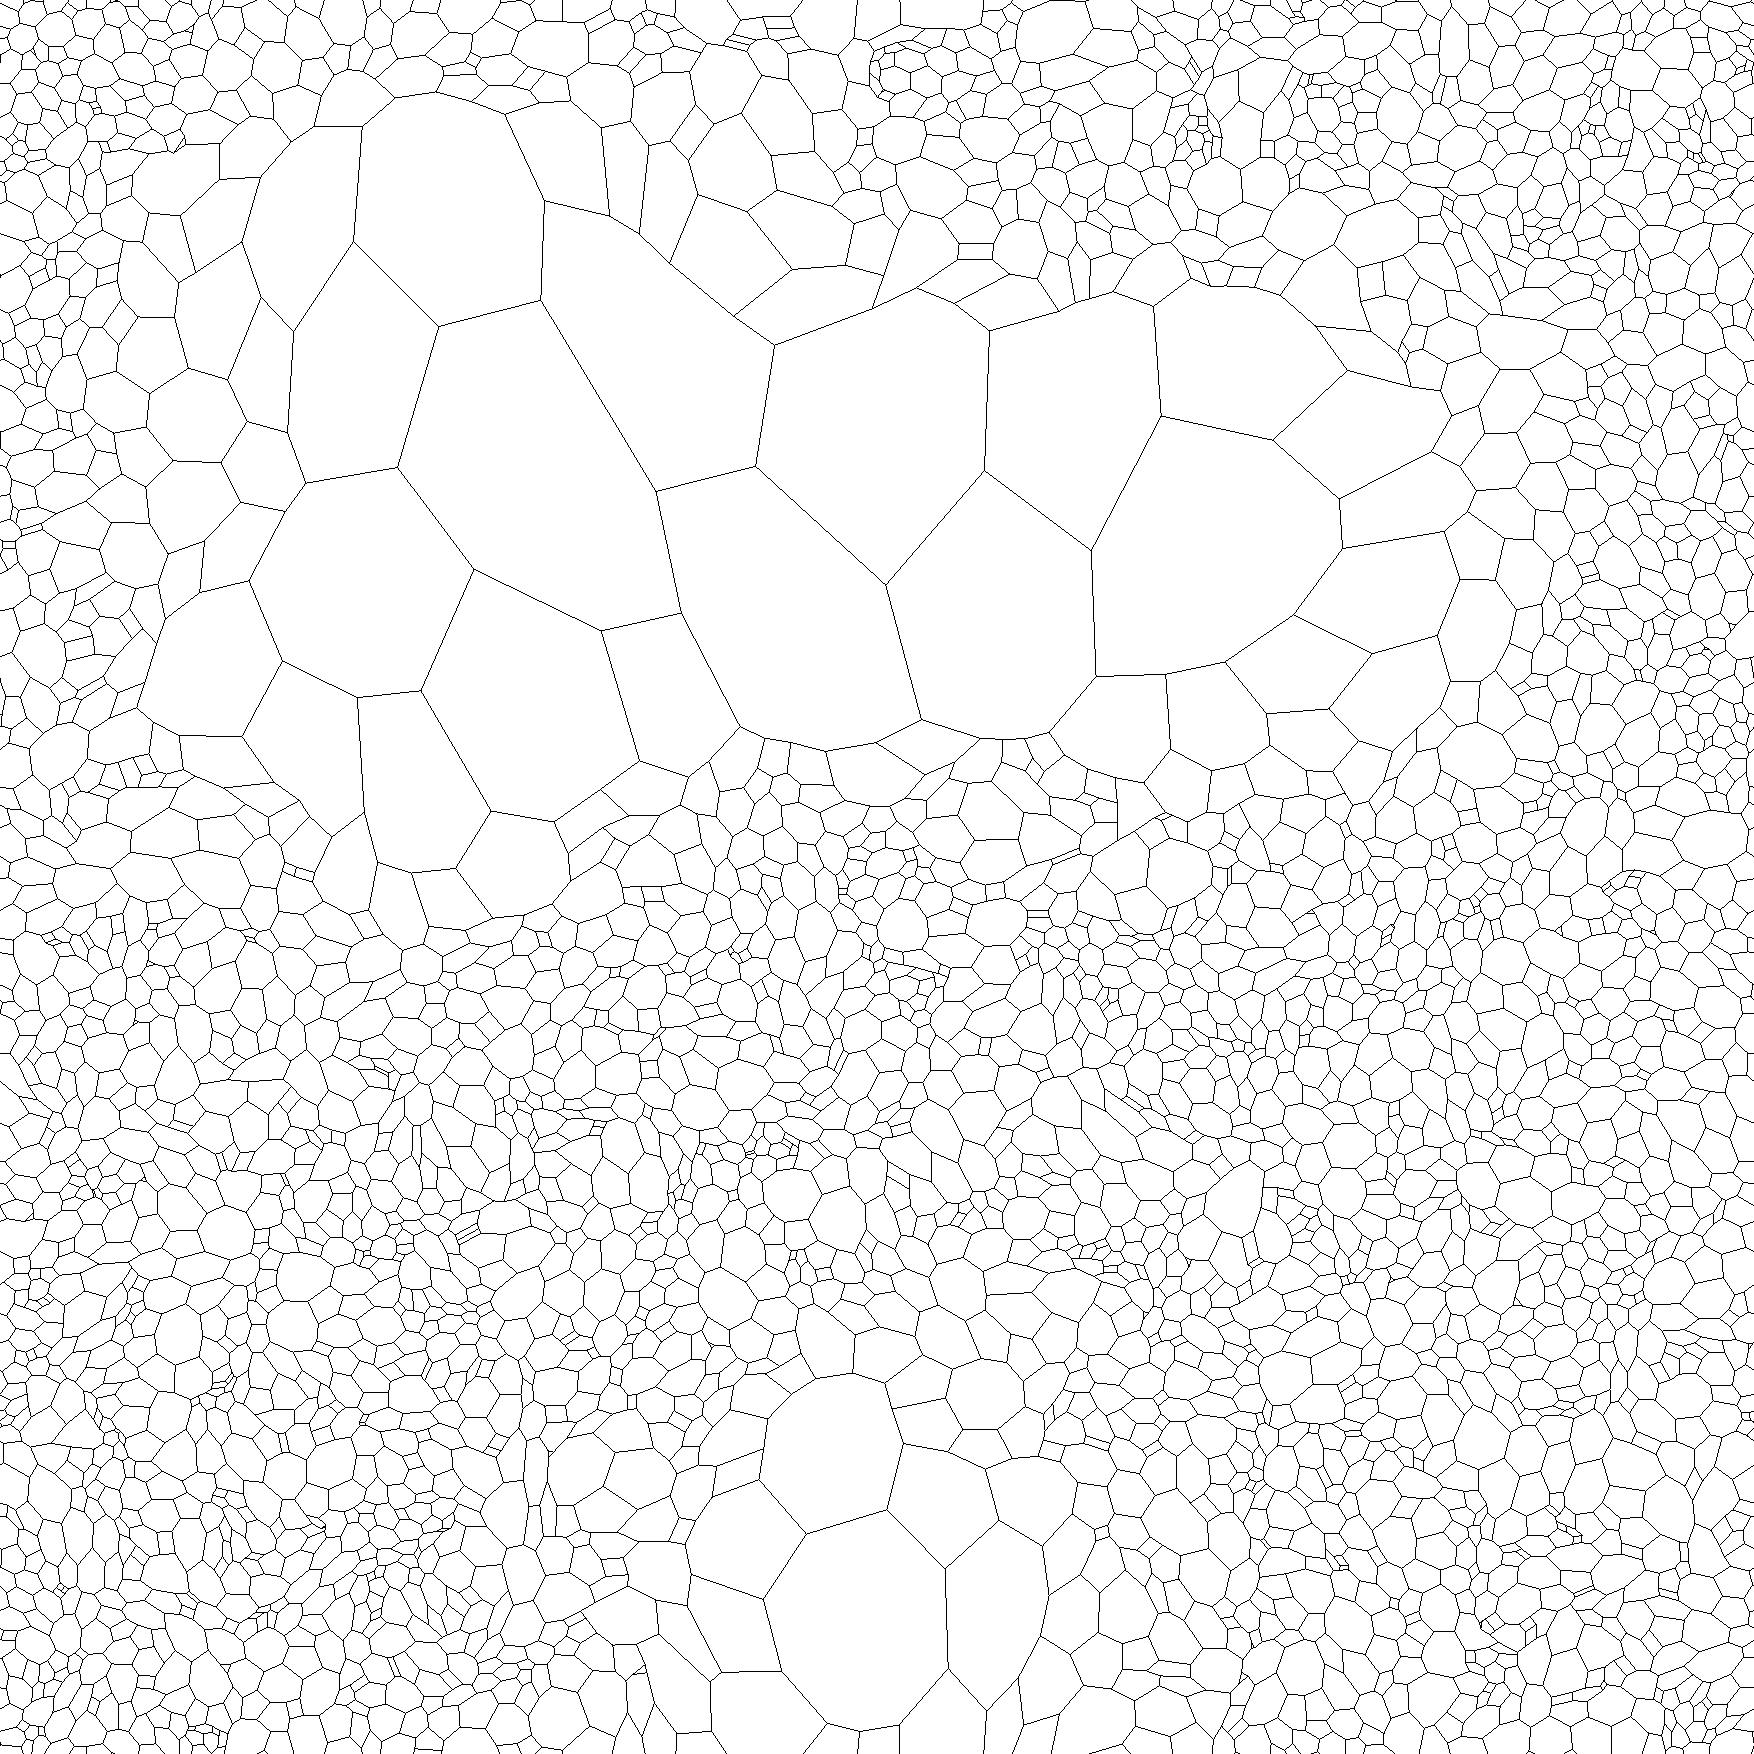
\includegraphics[width=297mm, height=297mm]{figure_code/test.pdf}}}
\BgThispage
\hypertarget{contributions}{%
\section{Contributions}\label{contributions}}

The material in this chapter expands on work presented in

\textbf{Insert citation of amorphous Kitaev paper here}

which was a joint project of the first three authors with advice and guidance from Willian and Johannes. The project grew out of an interest Gino, Peru and I had in studying amorphous systems, coupled with Johannes' expertise on the Kitaev model. The idea to use voronoi partitions came from \autocite{marsalTopologicalWeaireThorpe2020} and Gino did the implementation of this. The idea and implementation of the edge colouring using SAT solvers, the mapping from flux sector to bond sector using A* search were both entirely my work. Peru came up with the ground state conjecture and implemented the local markers. Gino and I did much of the rest of the programming for Koala while pair programming and 'whiteboard'ing, this included the phase diagram, edge mode and finite temperature analyses as well as the derivation of the projector in the amorphous case.

\hypertarget{introduction}{%
\section{Introduction}\label{introduction}}

The Kitaev Honeycomb model is remarkable because it combines three key properties.

First, this model is a plausible tight binding Hamiltonian. The form of the Hamiltonian could be realised by a real material. Candidate materials are known that are expected to behave according to the Kitaev with small corrections such as \(\alpha\mathrm{-RuCl}_3\) \autocite{banerjeeProximateKitaevQuantum2016,trebstKitaevMaterials2022}.

Second, this model is deeply interesting to modern condensed matter theory. Its ground state is almost the canonical example of the long sought after quantum spin liquid state. Its excitations are anyons, particles that can only exist in two dimensions that break the normal fermion/boson dichotomy. Anyons have been the subject of much attention because, among other reasons, they can be braided through spacetime to achieve noise tolerant quantum computations \textcite{freedmanTopologicalQuantumComputation2003}.

Third, and perhaps most importantly, this model is a rare many body interacting quantum system that can be treated analytically. It is exactly solvable. We can explicitly write down its many body ground states in terms of single particle states \textcite{kitaevAnyonsExactlySolved2006}. Its solubility comes about because the model has many conserved degrees of freedom that mediate the interactions between quantum degrees of freedom.

\hypertarget{amorphous-systems}{%
\subsection{Amorphous Systems}\label{amorphous-systems}}

\textbf{Insert discussion of why a generalisation to the amorphous case is interesting}

This chapter details the physics of the Kitaev model on amorphous lattices.

It starts by expanding on the physics of the Kitaev model. It will look at the gauge symmetries of the model as well as its solution via a transformation to a Majorana hamiltonian. This discussion shows that, for the the model to be solvable, it needs only be defined on a trivalent, tri-edge-colourable lattice \autocite{Nussinov2009}.

The methods section discusses how to generate such lattices and colour them. It also explain how to map back and forth between configurations of the gauge field and configurations of the gauge invariant quantities.

The results section begins by looking at the zero temperature physics. It presents numerical evidence that the ground state of the Kitaev model is given by a simple rule depending only on the number of sides of each plaquette. It assesses the gapless, Abelian and non-Abelian, phases that are present, characterising them by the presence of a gap and using local Chern markers. Next it looks at spontaneous chiral symmetry breaking and topological edge states. It also compares the zero temperature phase diagram to that of the Kitaev Honeycomb Model. Next, it takes the model to finite temperature and demonstrates that there is a phase transition to a thermal metal state.

The discussion considers possible physical realisations of this model and the motivations for doing so. It also discusses how a well known quantum error correcting code defined on the Kitaev Honeycomb model could be generalised to the amorphous case.

\hypertarget{glossary}{%
\subsection{Glossary}\label{glossary}}

\begin{itemize}
\item
  Lattice: The underlying graph on which the models are defined. Composed of sites (vertices), bonds (edges) and plaquettes (faces).
\item
  The model : Used when I refer to properties of the the Kitaev model that do not depend on the particular lattice.
\item
  The Honeycomb model : The Kitaev Model defined on the honeycomb lattice.
\item
  The Amorphous model : The Kitaev Model defined on the amorphous lattices described here.
\item
  The Hamiltonian: I will use model to refer to the underlying physics and Hamiltonian to refer to particular representations of the model.
\end{itemize}

\textbf{The Spin Hamiltonian}

\begin{itemize}
\tightlist
\item
  Spin Bond Operators: \(\hat{k}_{ij} = \sigma_i^\alpha \sigma_j^\alpha\)
\item
  Loop Operators: \(\hat{W_p} = \prod_{<i,j>} k_{ij}\)
\item
  Plaquette Operators: Loops that enclose a single plaquette.
\end{itemize}

\textbf{The Majorana Model}

\begin{itemize}
\tightlist
\item
  Majorana Operators on site \(i\): \(\hat{b}^x_i, \hat{b}^y_i, \hat{b}^z_i, \hat{c}_i\)
\item
  Majorana Bond Operators: \(\hat{u}_{ij} = i \sigma_i^\alpha \sigma_j^\alpha\)
\item
  Loop Operators: \(\hat{W_p} = \prod_{<i,j>} u_{ij}\)
\item
  Plaquette Operators: Loops that enclose a single plaquette.
\item
  Gauge Operators: \(D_i = \hat{b}^x_i \hat{b}^y_i \hat{b}^z_i \hat{c}_i\)
\item
  The Extended Hilbert space: The larger Hilbert space spanned by the Majorana operators.
\item
  The physical subspace: The subspace of the extended Hilbert space that we identify with the Hilbert space of the original spin model.
\item
  The Projector \(\hat{P}\): The projector onto the physical subspace.
\end{itemize}

\textbf{Flux Sectors}

\begin{itemize}
\item
  Odd/Even Plaquettes: Plaquettes with an odd/even number of sides.
\item
  Fluxes \(\phi_i\): The expectation values of the plaquette operators \(\pm 1\) for even and \(\pm i\) for odd plaquettes.
\item
  Flux Sector: A subspace of Hilbert space in which the fluxes take particular values.
\item
  Ground state flux sector: The Flux Sector containing the lowest energy many body state.
\item
  Vortices: Flux excitations away from the ground state flux sector.
\item
  Dual Loops: A set of \(u_{jk}\) that correspond to loops on the dual lattice.
\item
  non-contractible loops or dual loops: The two loops topologically distinct loops on the torus that cannot be smoothly deformed to a point.
\item
  Topological Fluxes \(\Phi_{x}, \Phi_{y}\): The two fluxes associated with the two non-contractible loops.
\item
  Topological Transport Operators: \(\mathcal{T}_{x}, \mathcal{T}_{y}\): The two vortex-pair operations associated with the non-contractible \emph{dual} loops.
\end{itemize}

\textbf{Phases}

\begin{itemize}
\tightlist
\item
  The A phase: The three anisotropic regions of the phase diagram \(A_x, A_y, A_z\) where \(A_\alpha\) means \(J_\alpha >> J_\beta, J_\gamma\).
\item
  The B phase: The roughly isotropic region of the phase diagram.
\end{itemize}

\hypertarget{the-kitaev-model}{%
\subsection{The Kitaev Model}\label{the-kitaev-model}}

\hypertarget{commutation-relations}{%
\subsubsection{Commutation relations}\label{commutation-relations}}

Before diving into the Hamiltonian of the Kitaev model, the following describes the key commutation relations of spins, fermions and Majoranas.

\hypertarget{spins}{%
\paragraph{Spins}\label{spins}}

Skip this is you are familiar with the algebra of the Pauli matrices. Scalars like \(\delta_{ij}\) should be understood to be multiplied by an implicit identity \(\mathbb{1}\) where necessary.

We can represent a single spin\(-1/2\) particle using the Pauli matrices \((\sigma^x, \sigma^y, \sigma^z) = \vec{\sigma}\), these matrices all square to the identity \(\sigma^\alpha \sigma^\alpha = \mathbb{1}\) and obey nice commutation and exchange rules: \[\sigma^\alpha \sigma^\beta = \delta^{\alpha \beta} + i \epsilon^{\alpha \beta \gamma} \sigma^\gamma\] \[[\sigma^\alpha, \sigma^\beta] = 2 i \epsilon^{\alpha \beta \gamma} \sigma^\gamma\]

Adding site indices, spins at different spatial sites always commute \([\vec{\sigma}_i, \vec{\sigma}_j] = 0\) so when \(i \neq j\) \[\sigma_i^\alpha \sigma_j^\beta = \sigma_j^\alpha \sigma_i^\beta\] \[[\sigma_i^\alpha, \sigma_j^\beta] = 0\] while the previous equations hold for \(i = j\).

Two extra relations useful for the Kitaev model are the value of \(\sigma^\alpha \sigma^\beta \sigma^\gamma\) and \([\sigma^\alpha \sigma^\beta, \sigma^\gamma]\) when \(\alpha \neq \beta \neq \gamma\) these can be computed relatively easily by applying the above relations yielding: \[\sigma^\alpha \sigma^\beta \sigma^\gamma = i \epsilon^{\alpha\beta\gamma}\] and \[[\sigma^\alpha \sigma^\beta, \sigma^\gamma] = 0\]

\hypertarget{fermions-and-majoranas}{%
\paragraph{Fermions and Majoranas}\label{fermions-and-majoranas}}

The fermionic creation and anhilation operators are defined by the canonical anticommutation relations \[\begin{aligned}
\{f_i, f_j\} &= \{f^\dagger_i, f^\dagger_j\} = 0\\
\{f_i, f^\dagger_j\} &= \delta_{ij}
\end{aligned}\] which give us the exchange statistics and Pauli exclusion principle.

From fermionic operators, we can construct Majorana operators: \[\begin{aligned}
f_i         &= 1/2 (a_i + ib_i)\\
f^\dagger_i &= 1/2(a_i - ib_i)\\
a_i         &= f_i + f^\dagger_i = 2\Re f\\
b_i         &= 1/i(f_i - f^\dagger_i) = 2\Im f 
\end{aligned}\]

Majorana operators are the real and imaginary parts of the fermionic operators. Physically, they correspond to the orthogonal superpositions of the presence and absence of the fermion and are, thus, a kind of quasiparticle.

Once we involve multiple fermions, there is some freedom in how we can perform the transformation from \(n\) fermions \(f_i\) to \(2n\) Majoranas \(c_i\). The property that must be preserved, however, is that the Majoranas still anticommute:

\[ \{c_i, c_j\} = 2\delta_{ij}\]

\begin{figure}
\hypertarget{fig:visual_kitaev_1}{%
\centering
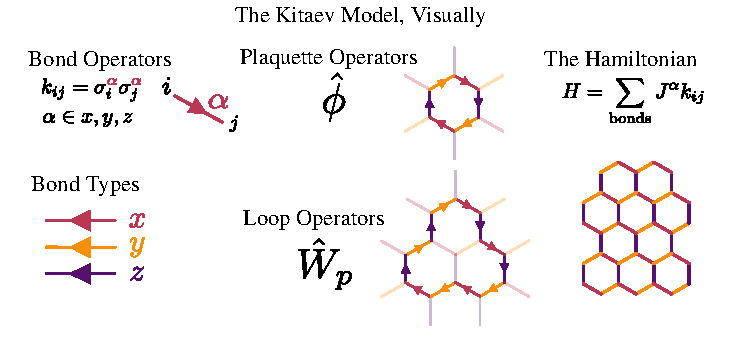
\includegraphics[width=1\textwidth,height=\textheight]{figure_code/amk_chapter/visual_kitaev_1.pdf}
\caption{A visual introduction to the Kitaev Model.}\label{fig:visual_kitaev_1}
}
\end{figure}

\hypertarget{the-hamiltonian}{%
\subsubsection{The Hamiltonian}\label{the-hamiltonian}}

To start from the fundamentals, the Kitaev Honeycomb model is a model of interacting spin\(-1/2\)s on the vertices of a honeycomb lattice. Each bond in the lattice is assigned a label \(\alpha \in \{ x, y, z\}\) and that bond couples its two spin neighbours along the \(\alpha\) axis. See \cref{fig:visual_kitaev_1} for a diagram.

This gives us the Hamiltonian \[H =  - \sum_{\langle j,k\rangle_\alpha} J^{\alpha}\sigma_j^{\alpha}\sigma_k^{\alpha},\] where \(\sigma^\alpha_j\) is a Pauli matrix acting on site \(j\) and \(\langle j,k\rangle_\alpha\) is a pair of nearest-neighbour indices connected by an \(\alpha\)-bond with exchange coupling \(J^\alpha\) \textcite{kitaevAnyonsExactlySolved2006}. For notational brevity, it is useful to introduce the bond operators \(K_{ij} = \sigma_j^{\alpha}\sigma_k^{\alpha}\) where \(\alpha\) is a function of \(i,j\) that picks the correct bond type.

This Kitaev model has a set of conserved quantities that, in the spin language, take the form of Wilson loop operators \(W_p\) winding around a closed path on the lattice. The direction does not matter, but we will keep to clockwise here. We will use the term plaquette and the symbol \(\phi\) to refer to a Wilson loop operator that does not enclose any other sites, such as a single hexagon in a honeycomb lattice.

\[W_p = \prod_{\mathrm{i,j}\; \in\; p} K_{ij} = \sigma_1^z \sigma_2^x \sigma_2^y \sigma_3^y .. \sigma_n^y \sigma_n^y \sigma_1^z\]

\textbf{add a diagram of a single plaquette with labelled site and bond types}

In closed loops, each site appears twice in the product with two of the three bond types. Applying \(\sigma^\alpha \sigma^\beta = \epsilon^{\alpha \beta \gamma} \sigma^\gamma, \alpha \neq \beta\) then gives us a product containing a single Pauli matrix associated with each site in the loop with the type of the \emph{outward} pointing bond. This shows that the \(W_p\) associated with hexagons or shapes with an even number of sides all square to 1 and, hence, have eigenvalues \(\pm 1\).

A bipartite lattice is composed of A and B sublattices with no intra-sublattice edges, i.e.~no A-A or B-B edges. Any closed loop must begin and end at the same site. If we start at an A site, the loop must go A-B-A-B\ldots{} until it returns to the original site. It must, therefore, contain an even number of edges to end on the same sublattice that it started on.

As the honeycomb lattice is bipartite, there are no closed loops that contain an even number of edges. Therefore, all the \(W_p\) have eigenvalues \(\pm 1\) on bipartite lattices. Later, we will show that plaquettes with an odd number of sides (odd plaquettes for short) have eigenvalues \(\pm i\).

\begin{figure}
\hypertarget{fig:regular_plaquettes}{%
\centering
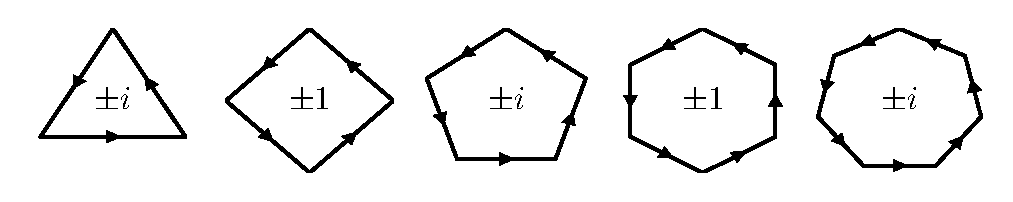
\includegraphics[width=0.86\textwidth,height=\textheight]{figure_code/amk_chapter/intro/regular_plaquettes/regular_plaquettes.pdf}
\caption{The eigenvalues of a loop or plaquette operators depend on the number of bonds in its enclosing path.}\label{fig:regular_plaquettes}
}
\end{figure}

Remarkably, all of the spin bond operators \(K_{ij}\) commute with all the Wilson loop operators \(W_p\). \[[W_p, J_{ij}] = 0\] We can prove this by considering three cases: 1. neither \(i\) nor \(j\) is part of the loop 2. one of \(i\) or \(j\) are part of the loop 3. both are part of the loop

The first case is trivial. The other two require some algebra, outlined in \cref{fig:visual_kitaev_2}.

\begin{figure}
\hypertarget{fig:visual_kitaev_2}{%
\centering
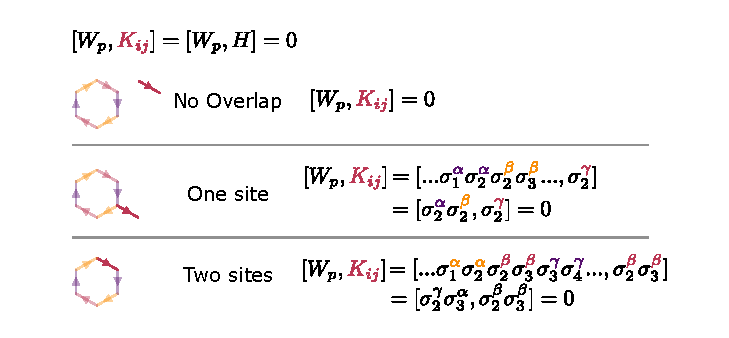
\includegraphics[width=1\textwidth,height=\textheight]{figure_code/amk_chapter/visual_kitaev_2.pdf}
\caption{Plaquette operators are conserved.}\label{fig:visual_kitaev_2}
}
\end{figure}

Since the Hamiltonian is a linear combination of bond operators, it commutes with the plaquette operators. This is helpful because it leads to a simultaneous eigenbasis for the Hamiltonian and the plaquette operators. We can, thus, work in \emph{or ``on''???} a basis in which the eigenvalues of the plaquette operators take on a definite value and, for all intents and purposes, act like classical degrees of freedom. These are the extensively many conserved quantities that make the model tractable.

Plaquette operators measure flux. We will find that the ground state of the model corresponds to some particular choice of flux through each plaquette. We will refer to excitations which flip the expectation value of a plaquette operator away from the ground state as \textbf{vortices}.

Thus, fixing a configuration of the vortices partitions the many-body Hilbert space into a set of `vortex sectors' labelled by that particular flux configuration \(\phi_i = \pm 1,\pm i\).

\hypertarget{from-spins-to-majorana-operators}{%
\subsubsection{From Spins to Majorana operators}\label{from-spins-to-majorana-operators}}

\hypertarget{for-a-single-spin}{%
\paragraph{For a single spin}\label{for-a-single-spin}}

Let us start by considering only one site and its \(\sigma^x, \sigma^y\) and \(\sigma^z\) operators which live in a two dimensional Hilbert space \(\mathcal{L}\).

We will introduce two fermionic modes \(f\) and \(g\) that satisfy the canonical anticommutation relations along with their number operators \(n_f = f^\dagger f, n_g = g^\dagger g\) and the total fermionic parity operator \(F_p = (2n_f - 1)(2n_g - 1)\) which can be used to divide their Fock space up into even and odd parity subspaces. These subspaces are separated by the addition or removal of one fermion.

From these two fermionic modes, we can build four Majorana operators: \[\begin{aligned}
b^x &= f + f^\dagger\\
b^y &= -i(f - f^\dagger)\\
b^z &= g + g^\dagger\\
c   &= -i(g - g^\dagger)
\end{aligned}\]

The Majoranas obey the usual commutation relations, squaring to one and anticommuting with each other. The fermions and Majorana live in a four dimensional Fock space \(\mathcal{\tilde{L}}\). We can therefore identify the two dimensional space \(\mathcal{M}\) with one of the parity subspaces of \(\mathcal{\tilde{L}}\) which will be called the \emph{physical subspace} \(\mathcal{\tilde{L}}_p\). Kitaev defines the operator \[D = b^xb^yb^zc\] which can be expanded to \[D = -(2n_f - 1)(2n_g - 1) = -F_p\] and labels the physical subspace as the space spanned by states for which \[ D|\phi\rangle = |\phi\rangle\]

We can also think of the physical subspace as whatever is left after applying the projector \[P  = \frac{1 - D}{2}\] This formulation will be useful for taking states that span the extended space \(\mathcal{\tilde{M}}\) and projecting them into the physical subspace.

So now, with the caveat that we are working in the physical subspace, we can define new Pauli operators:

\[\tilde{\sigma}^x = i b^x c,\; \tilde{\sigma}^y = i b^y c,\; \tilde{\sigma}^y = i b^y c\]

These extended space Pauli operators satisfy all the usual commutation relations. The only difference is that if we evaluate \(\sigma^x \sigma^y \sigma^z = i\), we instead get \[ \tilde{\sigma}^x\tilde{\sigma}^y\tilde{\sigma}^z = iD \]

This makes sense if we promise to confine ourselves to the physical subspace \(D = 1\).

\hypertarget{for-multiple-spins}{%
\paragraph{For multiple spins}\label{for-multiple-spins}}

This construction easily generalises to the case of multiple spins. We get a set of 4 Majoranas \(b^x_j,\; b^y_j,\;b^z_j,\; c_j\) and a \(D_j = b^x_jb^y_jb^z_jc_j\) operator for every spin. For a state to be physical, we require that \(D_j |\psi\rangle = |\psi\rangle\) for all \(j\).

From these each Pauli operator can be constructed: \[\tilde{\sigma}^\alpha_j = i b^\alpha_j c_j\]

This is where the magic happens. We can promote the spin hamiltonian from \(\mathcal{L}\) into the extended space \(\mathcal{\tilde{L}}\), safe in the knowledge that nothing changes so long as we only actually work with physical states. The Hamiltonian \[\begin{aligned}
\tilde{H} &=  - \sum_{\langle j,k\rangle_\alpha} J^{\alpha}\tilde{\sigma}_j^{\alpha}\tilde{\sigma}_k^{\alpha}\\
          &= \frac{i}{4} \sum_{\langle j,k\rangle_\alpha} 2J^{\alpha} (ib^\alpha_i b^\alpha_j) c_i c_j\\
          &=  \frac{i}{4} \sum_{\langle i,j\rangle_\alpha} 2J^{\alpha} \hat{u}_{ij} \hat{c}_i \hat{c}_j
\end{aligned}\]

We can factor out the Majorana bond operators \(\hat{u}_{ij} = i b^\alpha_i b^\alpha_j\). Note that these bond operators are not equal to the spin bond operators \(K_{ij} = \sigma^\alpha_i \sigma^\alpha_j = - \hat{u}_{ij} c_i c_j\). In what follows, we will work much more frequently with the Majorana bond operators. Therefore, when we refer to bond operators without qualification, we are referring to the Majorana variety.

Similarly to the argument with the spin bond operators \(K_{ij}\), we can quickly verify by considering three cases that the Majorana bond operators \(u_{ij}\) all commute with one another. They square to one, so have eigenvalues \(\pm 1\). They also commute with the \(c_i\) operators.

Importantly, the operators \(D_i = b^x_i b^y_i b^z_i c_i\) commute with \(K_{ij}\) and, therefore, with \(\tilde{H}\). We will show later that the action of \(D_i\) on a state is to flip the values of the three \(u_{ij}\) bonds that connect to site \(i\). Physically, this indicates that \(u_{ij}\) is a gauge field with a high degree of degeneracy.

In summary, Majorana bond operators \(u_{ij}\) are an emergent, classical, \(\mathbb{Z_2}\) gauge field!

\hypertarget{partitioning-the-hilbert-space-into-bond-sectors}{%
\subsubsection{Partitioning the Hilbert Space into Bond sectors}\label{partitioning-the-hilbert-space-into-bond-sectors}}

Similarly to the story with the plaquette operators from the spin language, we can divide the Hilbert space \(\mathcal{L}\) into sectors labelled by a set of choices \(\{\pm 1\}\) for the value of each \(u_{ij}\) operator which we denote by \(\mathcal{L}_u\). Since \(u_{ij} = -u_{ji}\), we can represent the \(u_{ij}\) graphically with an arrow that points along each bond in the direction in which \(u_{ij} = 1\).

Once confined to a particular \(\mathcal{L}_u\), we can `remove the hats' from the \(\hat{u}_{ij}\). The hamiltonian becomes a quadratic, free fermion problem \[\tilde{H_u} =  \frac{i}{4} \sum_{\langle i,j\rangle_\alpha} 2J^{\alpha} u_{ij} c_i c_j\] The ground state, \(|\psi_u\rangle\) can be found easily via matrix diagonalisation. At this point, we may wonder whether the \(\mathcal{L}_u\) are confined entirely within the physical subspace \(\mathcal{L}_p\) and, indeed, we will see that they are not. However, it will be helpful to first develop the theory of the Majorana Hamiltonian further.

\begin{figure}
\hypertarget{fig:intro_figure_by_hand}{%
\centering
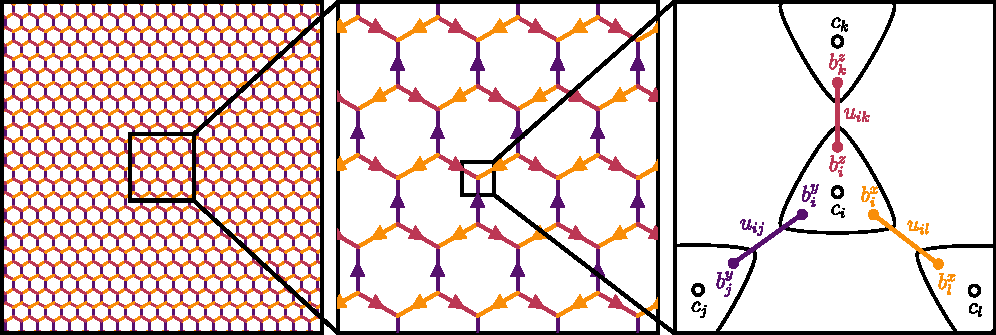
\includegraphics[width=1\textwidth,height=\textheight]{figure_code/amk_chapter/intro/honeycomb_zoom/intro_figure_by_hand.pdf}
\caption{\textbf{(a)} The standard Kitaev model is defined on a honeycomb lattice. The special feature of the honeycomb lattice that makes the model solvable is that each vertex is joined by exactly three bonds, i.e.~the lattice is trivalent. One of three labels is assigned to each \textbf{(b)}. We represent the antisymmetric gauge degree of freedom \(u_{jk} = \pm 1\) with arrows that point in the direction \(u_{jk} = +1\) \textbf{(c)}. The Majorana transformation can be visualised as breaking each spin into four Majoranas which then pair along the bonds. The pairs of x,y and z Majoranas become part of the classical \(\mathbb{Z}_2\) gauge field \(u_{ij}\). This leavies a single Majorana \(c_i\) per site.}\label{fig:intro_figure_by_hand}
}
\end{figure}

\hypertarget{the-majorana-hamiltonian}{%
\subsection{The Majorana Hamiltonian}\label{the-majorana-hamiltonian}}

We now have a quadratic Hamiltonian \[ \tilde{H} =  \frac{i}{4} \sum_{\langle i,j\rangle_\alpha} 2J^{\alpha} u_{ij} c_i c_j\] in which most of the Majorana degrees of freedom have paired along bonds to become a classical gauge field \(u_{ij}\). What follows is relatively standard theory for quadratic Majorana Hamiltonians \textcite{BlaizotRipka1986}.

Because of the antisymmetry of the matrix with entries \(J^{\alpha} u_{ij}\), the eigenvalues of the Hamiltonian \(\tilde{H}_u\) come in pairs \(\pm \epsilon_m\). This redundant information is a consequence of the doubling of the Hilbert space which occurred when we transformed to the Majorana representation.

If we organise the eigenmodes of \(H\) into pairs, such that \(b_m\) and \(b_m'\) have energies \(\epsilon_m\) and \(-\epsilon_m\), we can construct the transformation \(Q\) \[(c_1, c_2... c_{2N}) Q = (b_1, b_1', b_2, b_2' ... b_{N}, b_{N}')\] and put the Hamiltonian into the form \[\tilde{H}_u = \frac{i}{2} \sum_m \epsilon_m b_m b_m'\]

The determinant of \(Q\) will be useful later when we consider the projector from \(\mathcal{\tilde{L}}\) to \(\mathcal{L}\). Otherwise, the \(b_m\) are merely an intermediate step. From them, we form fermionic operators \[ f_i = \tfrac{1}{2} (b_m + ib_m')\] with their associated number operators \(n_i = f^\dagger_i f_i\). These let us write the Hamiltonian neatly as

\[ \tilde{H}_u = \sum_m \epsilon_m (n_m - \tfrac{1}{2}).\]

The ground state \(|n_m = 0\rangle\) of the many body system at fixed \(u\) is then \[E_{u,0} = -\frac{1}{2}\sum_m \epsilon_m \] We can construct any state from a particular choice of \(n_m = 0,1\).

If we only care about the value of \(E_{u,0}\), it is possible to skip forming the fermionic operators. The eigenvalues obtained directly from diagonalising \(J^{\alpha} u_{ij}\) come in \(\pm \epsilon_m\) pairs. We can take half the absolute value of the whole set to recover \(\sum_m \epsilon_m\) easily.

Takeaway: the Majorana Hamiltonian is quadratic within a Bond Sector.

\hypertarget{mapping-back-from-bond-sectors-to-the-physical-subspace}{%
\subsubsection{Mapping back from Bond Sectors to the Physical Subspace}\label{mapping-back-from-bond-sectors-to-the-physical-subspace}}

At this point, given a particular bond configuration \(u_{ij} = \pm 1\), we can construct a quadratic Hamiltonian \(\tilde{H}_u\) in the extended space and diagonalise it to find its ground state \(|\vec{u}, \vec{n} = 0\rangle\). This is not necessarily the ground state of the system as a whole, it is just the lowest energy state within the subspace \(\mathcal{L}_u\)

\textbf{However, \(|u, n_m = 0\rangle\) does not lie in the physical subspace}. As an example, consider the lowest energy state associated with \(u_{ij} = +1\). This state satisfies \[u_{ij} |\vec{u}=1, \vec{n} = 0\rangle = |\vec{u}=1, \vec{n} = 0\rangle\] for all bonds \(i,j\).

If we act on it, this state with one of the gauge operators \(D_j = b_j^x b_j^y b_j^z c_j\), we see that \(D_j\) flips the value of the three bonds \(u_{ij}\) that surround site \(k\):

\[ |u'\rangle = D_j |u=1, n_m = 0\rangle\]

\[ \begin{aligned}
\langle u'|u_{ij}|u'\rangle &=  \langle u| b_j^x b_j^y b_j^z c_j \;ib^x_i b^x_j\; b_j^x b_j^y b_j^z c_j|u\rangle\\
&= -1
\end{aligned}\]

Since \(D_j\) commutes with the Hamiltonian in the extended space \(\tilde{H}\), the fact that \(D_j\) flips the value of bond operators indicates that there is a gauge degeneracy between the ground state of \(\tilde{H}_u\) and the set of \(\tilde{H}_{u'}\) related to it by gauge transformations \(D_j\). Thus, we can flip any three bonds around a vertex and the physics will stay the same.

We can turn this into a symmetrisation procedure by taking a superposition of every possible gauge transformation. Every possible gauge transformation is just every possible subset of \({D_0, D_1 ... D_n}\) which can be neatly expressed as \[|\phi_w\rangle = \prod_i \left( \frac{1 + D_i}{2}\right) |\tilde{\phi}_u\rangle\] This is convenient because the quantity \(\frac{1 + D_i}{2}\) is also the local projector onto the physical subspace. Here \(|\phi_w\rangle\) is a gauge invariant state that lives in \(\mathcal{L}_p\) which has been constructed from a set of states in different \(\mathcal{L}_u\).

This gauge degeneracy leads us to the next topic of discussion, namely how to construct a set of gauge invariant quantities out of the \(u_{ij}\), these will turn out to just be the plaquette operators.

Takeaway: The Bond Sectors overlap with the physical subspace but are not contained within it.

\hypertarget{open-boundary-conditions}{%
\subsubsection{Open boundary conditions}\label{open-boundary-conditions}}

Care must be taken when defining open boundary conditions. Simply removing bonds from the lattice leaves behind unpaired \(b^\alpha\) operators that must be paired in some way to arrive at fermionic modes. To fix a pairing, we always start from a lattice defined on the torus and generate a lattice with open boundary conditions by defining the bond coupling \(J^{\alpha}_{ij} = 0\) for sites joined by bonds \((i,j)\) that we want to remove. This creates fermionic zero modes \(u_{ij}\) associated with these cut bonds which we set to 1 when calculating the projector.

Alternatively, since all the fermionic zero modes are degenerate anyway, an arbitrary pairing of the unpaired \(b^\alpha\) operators could be performed. \textless/i,j\textgreater\textless/i,j\textgreater{}

\hypertarget{gauge-fields}{%
\subsection{Gauge Fields}\label{gauge-fields}}

The bond operators \(u_{ij}\) are useful because they label a bond
sector \(\mathcal{\tilde{L}}_u\) in which we can easiy solve the
Hamiltonian. However the gauge operators move us between bond sectors.
\textbf{Bond sectors are not gauge invariant!}

Let's consider instead the properties of the plaquette operators
\(\hat{\phi}_i\) that live on the faces of the lattice.

We already showed that they are conserved. And as one might hope and
expect, the plaquette operators map cleanly on to the bond operators of
the Majorana representation:

\[\begin{aligned}
\tilde{W}_p &= \prod_{\mathrm{i,j}\; \in\; p} \tilde{K}_{ij}\\
            &= \prod_{\mathrm{i,j}\; \in\; p} \tilde{\sigma}_i^\alpha \tilde{\sigma}_j^\alpha\\
            &= \prod_{\mathrm{i,j}\; \in\; p} (ib^\alpha_i c_i)(ib^\alpha_j c_j)\\
            &= \prod_{\mathrm{i,j}\; \in\; p} i u_{ij} c_i c_j\\
            &= \prod_{\mathrm{i,j}\; \in\; p} i u_{ij}
\end{aligned}\]

Where the last steps holds because each \(c_i\) appears exactly twice
and adjacent to its neighbour in each plaquette operator. Note that this
is consistent with the observation from earlier that each \(W_p\) takes
values \(\pm 1\) for even paths and \(\pm i\) for odd paths.

\hypertarget{vortices-and-their-movements}{%
\subsubsection{Vortices and their
movements}\label{vortices-and-their-movements}}

Let's imagine we started from the ground state of the model and flipped
the sign of a single bond. In doing so we will flip the sign of the two
plaquettes adjacent to that bond. I'll call these disturbed plaquettes
\emph{vortices}. I'll refer to a particular choice values for the
plaquette operators as a vortex sector.

If we chain multiple bond flips we can create a pair of vortices at
arbitrary locations. The chain of bonds that we must flip corresponds to
a path on the dual of the lattice.

Something else we can do is create a pair of vortices, move one around a
loop and then anhilate it with its partner. This corresponds to a closed
loop on the dual lattice and applying such a bond flip leaves the vortex
sector unchanged.

Notice that the \(D_j\) operators flip three bonds around a vertex. This
is the smallest closed loop around which one can move a vortex pair and
anhilate it with itself.

Such operations compose in the sense that we can build any larger loop
by applying a series of \(D_j\) operations. Indeed the symetrisation
procedure \(\prod_i \left( \frac{1 + D_i}{2}\right)\) that maps from the
bond sector to a physical state is applying constructing a superposition
over every such loop that leaves the vortex sector unchanged.

The only loops that we cannot build out of \(D_j\)s are non-contractible
loops, such as those that span the major or minor circumference of the
torus.

\textbf{The plaquette operators are the gauge invariant quantity that
determines the physics of the model}

\hypertarget{composition-of-u_jk-loops}{%
\subsubsection{\texorpdfstring{Composition of \(u_{jk}\)
loops}{Composition of u\_\{jk\} loops}}\label{composition-of-u_jk-loops}}

\begin{figure}
\hypertarget{fig:plaquette_addition_by_hand}{%
\centering
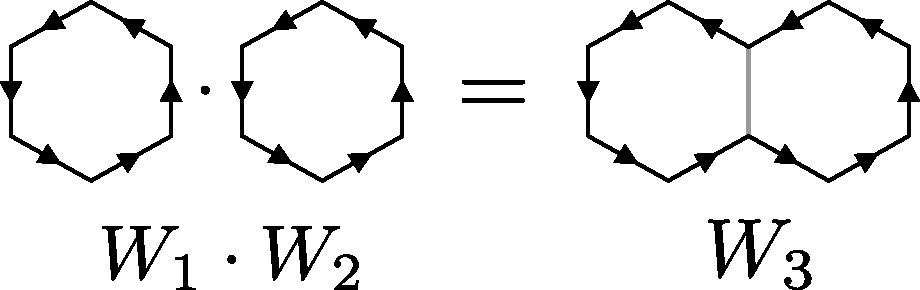
\includegraphics[width=0.57\textwidth,height=\textheight]{figure_code/amk_chapter/plaquette_addition/plaquette_addition_by_hand.pdf}
\caption{In the product of individual plaquette operators shared bonds
cancel out. The product is equal to the enclosing
path.}\label{fig:plaquette_addition_by_hand}
}
\end{figure}

Second it is now easy to show that the loops and plaquettes satisfy nice
composition rules, so long as we stick to loops that wind in a
particular direction.

Consider the product of two non-overlapping loops \(W_a\) and \(W_b\)
that share an edge \(u_{12}\). Since the two loops both wind clockwise
and do not overlap, one will contain a term \(i u_{12}\) and the other
\(i u_{21}\). Since the \(u_{ij}\) commute with one another, they square
to \(1\) and \(u_{ij} = -u_{ji}\) we see have \(i u_{12} i u_{21} = 1\)
and we can repeat this for any number of shared edges. Hence, we get a
version of Stokes' theorem: the product of \(i u_{jk}\) around any
closed loop \(\partial A\) is equal to the product of plaquette
operators \(\Phi\) that span the area \(A\) enclosed by that loop:
\[\prod_{u_{jk} \in \partial A} i \; u_{jk} = \prod_{\phi_i \in A} \phi_i\]

\begin{figure}
\hypertarget{fig:stokes_theorem}{%
\centering
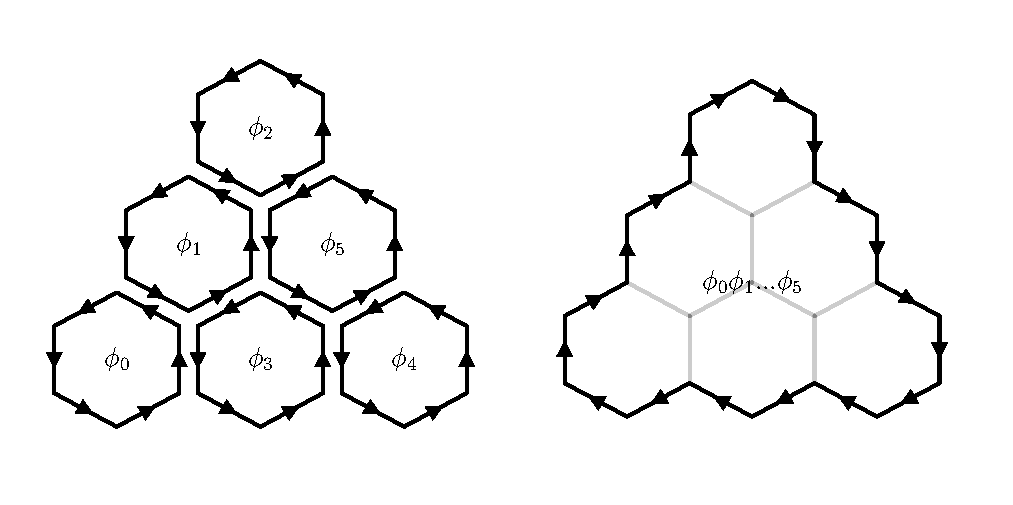
\includegraphics[width=0.71\textwidth,height=\textheight]{figure_code/amk_chapter/stokes_theorem/stokes_theorem.pdf}
\caption{The loop composition rule extends to arbitrary numbers of
vortices giving a discrete version of Stoke's
theorem.}\label{fig:stokes_theorem}
}
\end{figure}

\textbf{Wilson loops can always be decomposed into products of
plaquettes operators unless they are non-contractable}

\hypertarget{gauge-degeneracy-and-the-euler-equation}{%
\subsubsection{Gauge Degeneracy and the Euler
Equation}\label{gauge-degeneracy-and-the-euler-equation}}

We can check this analysis with a counting argument. For a lattice with
\(B\) bonds, \(P\) plaquettes and \(V\) vertices we can count how many
bond sectors, vortices sectors and gauge symmetries there are and check
them against Euler's polyhedra equation.

Euler's equation states for a closed surface of genus \(g\), i.e that
has \(g\) holes so \(0\) for the sphere, \(1\) for the torus and \(g\)
for \(g\) tori stuck together \[B = P + V + 2 - 2g\]

\begin{figure}
\hypertarget{fig:torus}{%
\centering
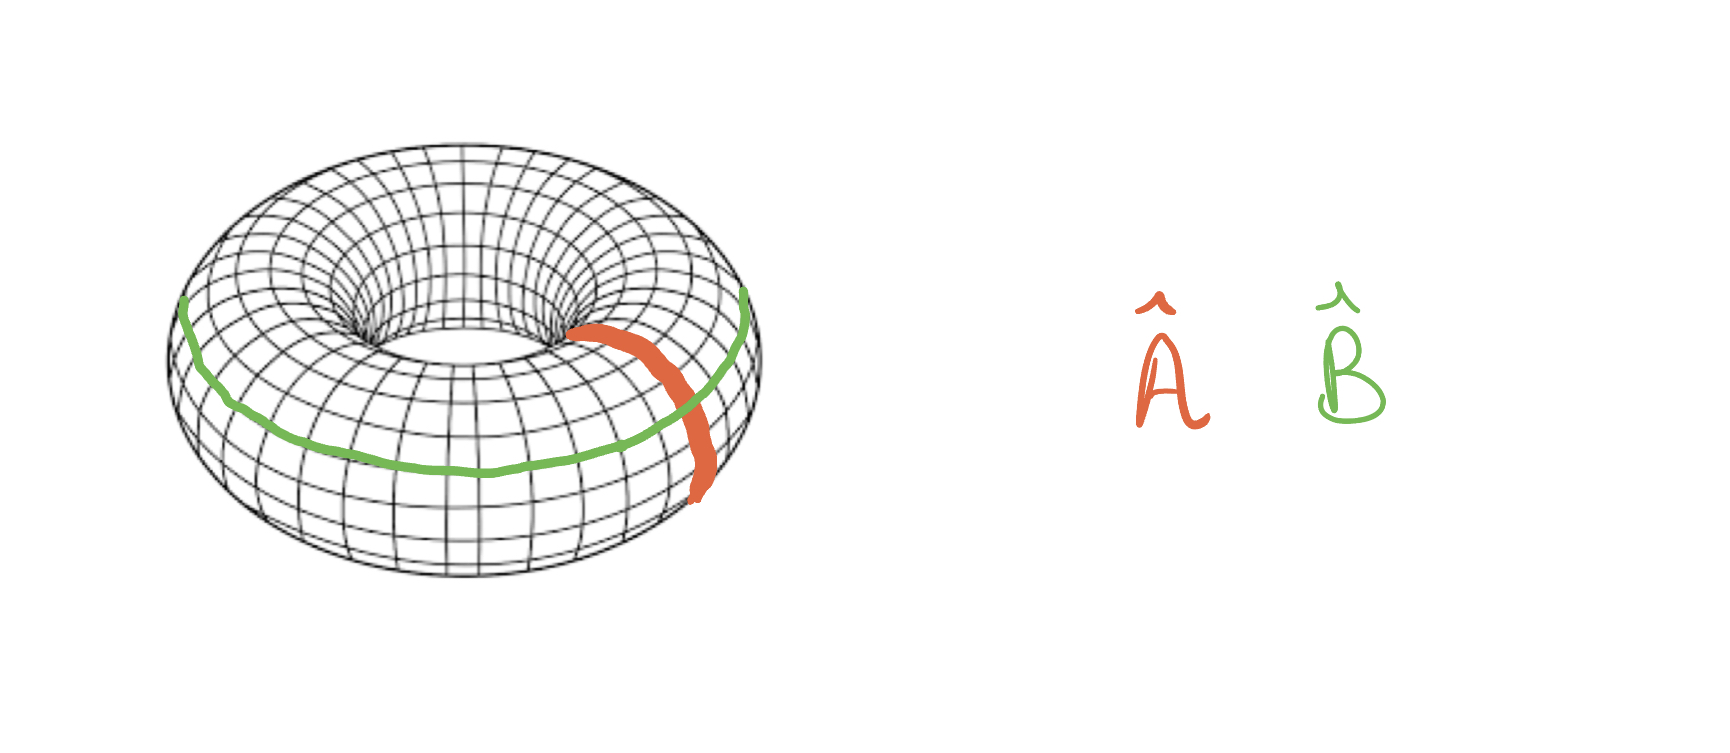
\includegraphics[width=0.86\textwidth,height=\textheight]{figure_code/amk_chapter/torus.jpeg}
\caption{In periodic boundary conditions the Kitaev model is defined on
the surface of a torus. Topologically the torus is distinct from the
sphere in that it has a hole that cannot be smoothly deformed away.
Associated with each such hole are two non-contractible loops on the
surface, here labeled A and B, that cannot be smoothly deformed to a
point. These two non-contracible loops can. be used to construct two
symmetry operators \(\hat{A}\) and \(\hat{A}\) that flip \(u_{jk}\)s
along their paths.}\label{fig:torus}
}
\end{figure}

For the case of the torus where \(g = 1\) we can rearrange this to read:
\[B = (P-1) + (V-1) + 2\]

Each \(u_{ij}\) takes two values and there is one associated with each
bond so there are exactly \(2^B\) distinct configurations of the bond
sector. Let's see if we can factor those configurations out into the
cartesian product of vortex sectors, gauge symmetries and
non-contractible loop operators.

Vortex sectors: each plaquette operator \(\phi_i\) takes two values
(\(\pm 1\) or \(\pm i\)) and there are \(P\) of them so naively one
would think there are \(2^P\). However vortices can only be created on
pairs so there are really \(\tfrac{2^P}{2} = 2^{P-1}\) vortex sectors.

Gauge symmetries: As discussed earlier these correspond to the all
possible compositions of the \(D_j\) operators. Again there are only
\(2^{V-1}\) of these because, as we will see in the next section,
\(\prod_{j} D_j = \mathbb{1}\) in the physical space, and we enforce
this by chooising the correct product of single particle fermion states.
You can get an intuitive picture for why \(\prod_{j} D_j = \mathbb{1}\)
by imagining larger and larger patches of \(D_j\) operators on the
torus. These patches correspond to transporting a vortex pair around the
edge of the patch. At some point the patch wraps around and starts to
cover the entire torus, as this happens the bounday of the patch
disappears and hence it which corresponds to the identity operation. See
Fig ?? (animated in the HTML version).

Finally the torus has two non-contractible loop operators asscociated
with its major and minor diameters.

Putting this all together we see that there are \textbf{\(2^B\) bond
sectors} a space which can be decomposed into the cartesian product of
\textbf{\(2^{P-1}\) vortex sectors}, \textbf{\(2^{V-1}\) gauge
symmetries} and \textbf{\(2^2 = 4\) topological sectors} associated with
the non-contractible loop operators. This last factor forms the basis of
proposals to construct topologically protected qubits since the 4
sectors cold only be mixed by a highly non-local perturbation, ref
?????.

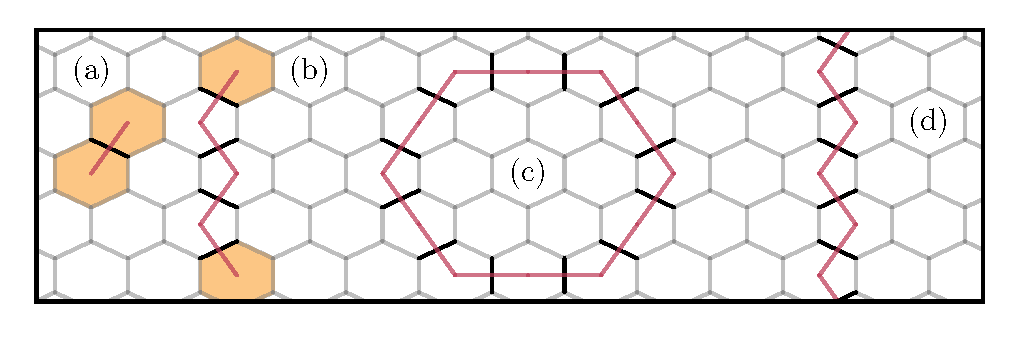
\includegraphics[width=1\textwidth,height=\textheight]{figure_code/amk_chapter/intro/types_of_dual_loops/types_of_dual_loops.pdf}
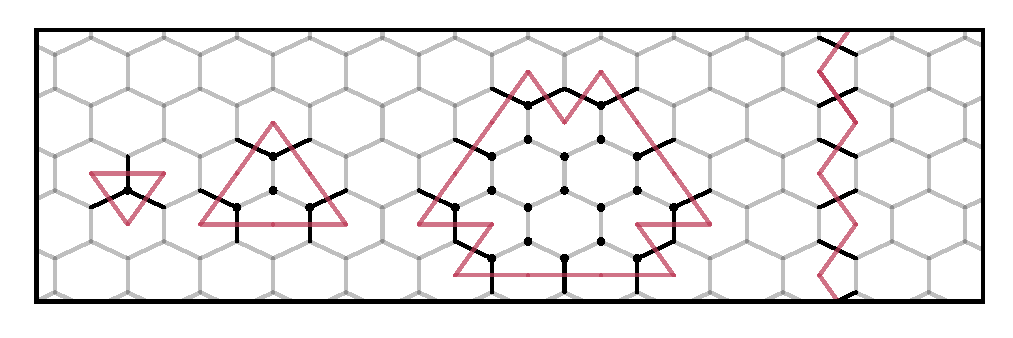
\includegraphics[width=1\textwidth,height=\textheight]{figure_code/amk_chapter/intro/gauge_symmetries/gauge_symmetries.pdf}
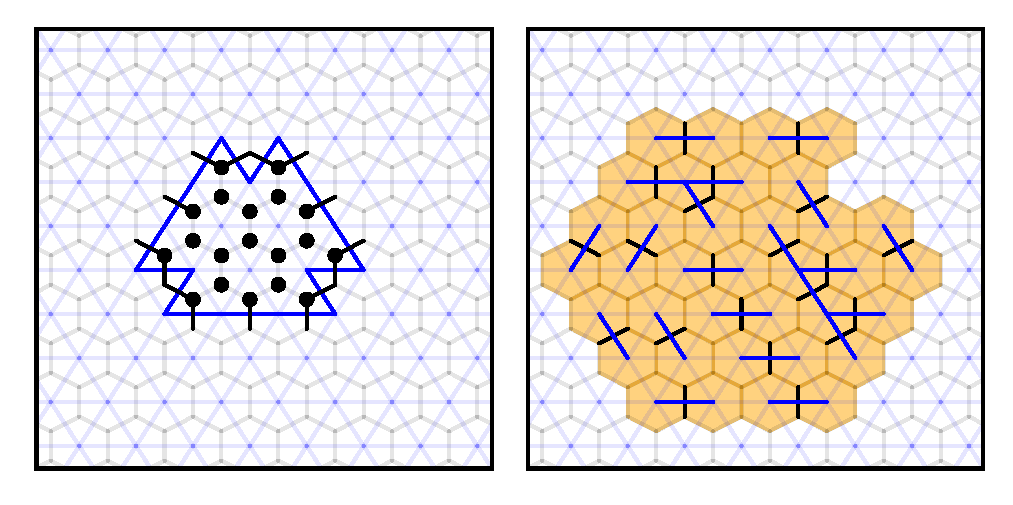
\includegraphics[width=1\textwidth,height=\textheight]{figure_code/amk_chapter/flood_fill/flood_fill.pdf}
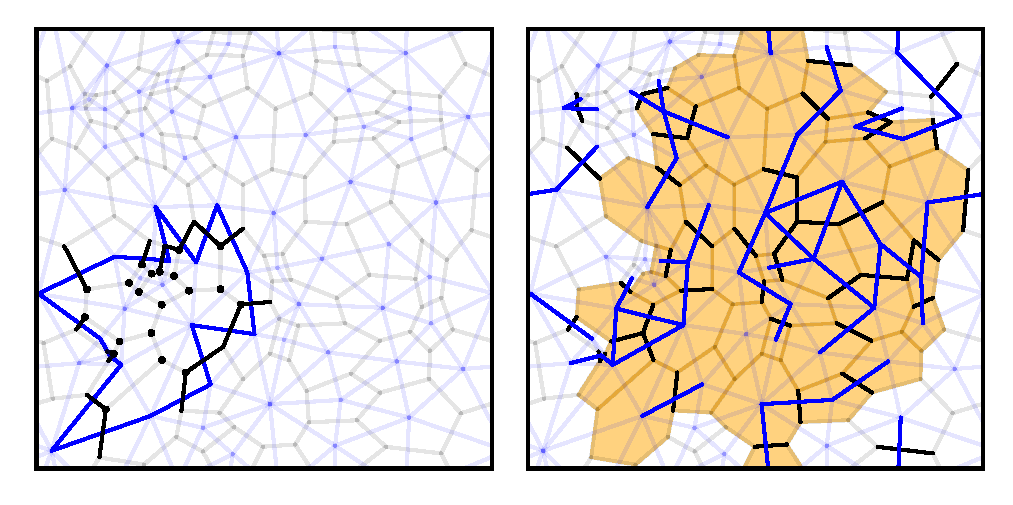
\includegraphics[width=1\textwidth,height=\textheight]{figure_code/amk_chapter/flood_fill_amorphous/flood_fill_amorphous.pdf}

\hypertarget{counting-edges-plaquettes-and-vertices}{%
\subsubsection{Counting edges, plaquettes and
vertices}\label{counting-edges-plaquettes-and-vertices}}

It will be useful to know how the trivalent structre of the lattice
constraints the number of bonds \(B\), plaquettes \(P\) and vertices
\(V\) it has.

We can immediately see that the lattice is built from vertices that each
share 3 edges with their neighbours. This means each vertex comes with
\(\tfrac{3}{2}\) bonds i.e \(3V = 2B\). This is consistent with the fact
that in the Majorana representation on the torus each vertex brings
three \(b^\alpha\) operators which then pair along bonds to give \(3/2\)
bonds per vertex.

If we define an integer \(N\) such that \(V = 2N\) and \(B = 3N\) and
substitite this into the polyhedra equation for the torus we see that
\(P = N\). So if is a trivalent lattice on the torus has \(N\)
plaquettes, it has \(2N\) vertices and \(3N\) bonds.

We can also consider the sum of the number of bonds in each plaquette
\(S_p\), since each bond is a member of exactly two plaquettes
\[S_p = 2B = 6N\]

The mean size of a plaquette in a trivalent lattice on the torus is
exactly 6. Since the sum is even, this also tells us that all odd
plaquettes must come in pairs.

\begin{figure}
\hypertarget{fig:hilbert_spaces}{%
\centering
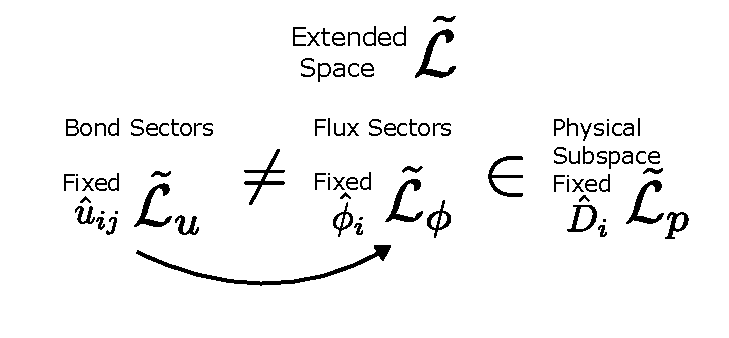
\includegraphics[width=1\textwidth,height=\textheight]{figure_code/amk_chapter/hilbert_spaces.pdf}
\caption{The relationship between the different Hilbert spaces used in
the solution is slightly complex.}\label{fig:hilbert_spaces}
}
\end{figure}

\hypertarget{the-projector}{%
\subsection{The Projector}\label{the-projector}}

It will turn out that the projection from the extended space to the
physical space is not actually that important for the results that I
will present. However it it useful to go through the theory of it to
explain why this is.

The physicil states are defined as those for which
\(D_i |\phi\rangle = |\phi\rangle\) for all \(D_i\). Since \(D_i\) has
eigenvalues \(\pm1\), the quantity \(\tfrac{(1+D_i)}{2}\) has eigenvalue
\(1\) for physical states and \(0\) for extended states so is the local
projector onto the physical subspace.

The global projector is therefore
\[ \mathcal{P} = \prod_{i=1}^{2N} \left( \frac{1 + D_i}{2}\right)\]

for a toroidal trivalent lattice with \(N\) plaquettes \(2N\) vertices
and \(3N\) edges. As I pointed out before the product over \((1 + D_j)\)
can also be thought of as the sum of all possible subsets \(\{i\}\) of
the \(D_j\) operators, which is the set of all possible gauge symmetry
operations.

\[ \mathcal{P} = \frac{1}{2^{2N}} \sum_{\{i\}} \prod_{i\in\{i\}} D_i\]

Since the gauge operators \(D_j\) commute and square to one, we can
define the complement operator \(C = \prod_{i=1}^{2N} D_i\) and see that
it take each set of \(\prod_{i \in \{i\}} D_j\) operators and gives us
the complement of that set. I said earlier that \(C\) is the identity in
the physical subspace and we will shortly see why.

We use the complement operator to rewrite the projector as a sum over
half the subsets of \(\{i\}\) let's call that \(\Lambda\). The
complement operator deals with the other half

\[ \mathcal{P} =  \left( \frac{1}{2^{2N-1}} \sum_{\Lambda} \prod_{i\in\{i\}} D_i\right) \left(\frac{1 + \prod_i^{2N} D_i}{2}\right) = \mathcal{S} \cdot \mathcal{P}_0\]

To compute \(\mathcal{P}_0\) the main quantity needed is the product of
the local projectors \(D_i\)
\[\prod_i^{2N} D_i = \prod_i^{2N} b^x_i b^y_i b^z_i c_i \] for a
toroidal trivalent lattice with \(N\) plaquettes \(2N\) vertices and
\(3N\) edges.

First we reorder the operators by bond type, this doesn't require any
information about the underlying lattice.

\[\prod_i^{2N} D_i = \prod_i^{2N} b^x_i \prod_i^{2N} b^y_i \prod_i^{2N} b^z_i \prod_i^{2N} c_i\]

The product over \(c_i\) operators reduces to a determinant of the Q
matrix and the fermion parity, see
\textcite{pedrocchiPhysicalSolutionsKitaev2011b}. The only difference
from the honeycomb case is that we cannot explicitely compute the
factors \(p_x,p_y,p_z = \pm\;1\) that arise from reordering the b
operators such that pairs of vertices linked by the corresponding bonds
are adjacent.

\[\prod_i^{2N} b^\alpha_i = p_\alpha \prod_{(i,j)}b^\alpha_i b^\alpha_j\]

However they are simply the parity of the permutation from one ordering
to the other and can be computed in linear time with a cycle
decomposition \textcite{app:cycle_decomp}.

We find that
\[\mathcal{P}_0 = 1 + p_x\;p_y\;p_z\; \hat{\pi} \; \mathrm{det}(Q^u) \; \prod_{\{i,j\}} -iu_{ij}\]

where \(p_x\;p_y\;p_z = \pm 1\) are lattice structure factors.
\(det(Q^u)\) is the determinant of the matrix mentioned earlier that
maps \(c_i\) operators to normal mode operators \(b'_i, b''_i\). These
depend only on the lattice structure.

\(\hat{\pi} = \prod{i}^{N} (1 - 2\hat{n}_i)\) is the parity of the
particular many body state determined by fermionic occupation numbers
\(n_i\). As discussed in
+\textcite{pedrocchiPhysicalSolutionsKitaev2011b} is \(\hat{\pi}\) is
gauge invariant in the sense that \([\hat{\pi}, D_i] = 0\).

This implies that \(det(Q^u) \prod -i u_{ij}\) is also a guage invariant
quantity. In translation invariant models this quantity which can be
related to the parity of the number of vortex pairs in the system
\textcite{yaoAlgebraicSpinLiquid2009}. However it is not so simple to
evaluate in the amorphous case.

More general
arguments\autocite{chungExplicitMonodromyMoore2007,oshikawaTopologicalDegeneracyNonAbelian2007}
imply that \(det(Q^u) \prod -i u_{ij}\) has an interesting relationship
to the topological fluxes. In the non-Abelian phase we expect that it
will change sign in exactly on of the four topological sectors. This
forces that sector that contain a fermion and hence gives the model a
three-fold degerenate ground state. In the Abelian phase this doesn't
happen and we get a fourfold degerate ground state. Whether this
analysis generalises to the amorphous case in unclear.

An alternate way to view this is to consider the adiabatic insertion of
the fluxes \(\Phi_{x,y}\) as the operations that undo vortex transport
around the lattice. In this picture the three fold degeneracy occurs
because transporting a vortex around \textbf{both} the major and minor
axes of the torus changes its fusion channel such that the two vortices
fuse into a fermion excition rather than the vacuum.

All these factors take values \(\pm 1\) so \(\mathcal{P}_0\) is 0 or 1
for a particular state. Since \(\mathcal{S}\) corresponds to
symmetrising over all the gauge configurations and cannot be 0, this
tells use that once we have determined the single particle eigenstates
of a bond sector, the true many body ground state has the same energy as
either the empty state with \(n_i = 0\) or a state with a single fermion
in the lowest level.

Let's think about where are with the model now. We can map the spin
Hamiltonian to a Majorana Hamiltonian in an extended Hilbert space.
Along with that mapping comes a gauge field \(u_{jk}\) defining
\textbf{bond sectors}. The gauge symmetries of \(u_{jk}\) are generated
by the set of \(D_j\) operators. The gauge invariant and therefore
physically relevant variables are the plaquette operators \(\phi_i\)
which define as a \textbf{vortex sector}. In order to practically solve
the Majorana Hamiltonian we must remove hats from the gauge field by
restricting ourselves to a particular bond sector. From there the
Majorana Hamiltonian becomes non-interacting and we can solve it like
any quadratic theory. This lets us construct the single particle
eigenstates from which we can also construct many body states. However
the many body states constructed this way are not in the physical
subspace!

However for the many body states within a particular bond sector,
\(\mathcal{P}_0 = 0,1\) tells us which of those have some overlap with
the physical sector.

We see that finding a state that has overlap with a physical state only
ever requires the addition or removal of one fermion. There are cases
where this can make a difference but for most observables such as ground
state energy this correction scales away as the number of fermions in
the system grows.

If we wanted to construct a full many body wavefunction in the spin
basis we would need to include the full symmetrisation over the gauge
fields. However this was not necessary for any of the results that will
be presented here.

\hypertarget{the-ground-state}{%
\subsection{The Ground State}\label{the-ground-state}}

As we have shown that the Hamiltonian is gauge invariant, only the flux
sector and the two topological fluxes affect the spectrum of the
Hamiltonian. Thus we can label many body ground state by a combination
of flux sector and fermionic occupation numbers.

By studying the projector we saw that the fermionic occupation numbers
of the ground state will always be either \(n_m = 0\) or
\(n_0 = 1, n_{m>1} = 0\) because the projector really just enforces
vortex and fermion parity.

I refer to the flux sector that contains the ground state as the ground
state flux sector. Recall that we call the excitations of the fluxes
away from the ground ground state configuration \textbf{vortices}, so
that the ground state flux sector is the vortex free sector by
definition.

On the Honeycomb, Lieb's theorem implies that the the ground state
corresponds to the state where all \(u_{jk} = 1\) implying that the flux
free sector is the ground state sector \textcite{lieb_flux_1994}.

Lieb's theorem does not generalise easily to the amorphous case. However
we can get some intuition by examining the problem that will lead to a
guess for the ground state. We will then provide numerical evidence that
this guess is in fact correct.

Let's consider the partition function of the Majorana hamiltonian:
\[ \mathcal{Z} = \mathrm{Tr}\left( e^{-\beta H}\right) = \sum_i \exp{-\beta \epsilon_i}\]
At low temperatures \(\mathcal{Z} \approx \beta \epsilon_0\) where
\(\epsilon_0\) is the lowest energy fermionic state.

How does the \(\mathcal{Z}\) depend on the Majorana hamiltonian?
Expanding the exponential out gives:
\[ \mathcal{Z} = \sum_n \frac{(-\beta)^n}{n!} \mathrm{Tr(H^k)} \]

Now there's an interesting observation to make here. The Hamiltonian is
essentially a scaled adjacency matrix. An adjacency matrix being a
matrix \(g_{ij}\) such that \(g_{ij} = 1\) if vertices \(i\) and \(j\)
and joined by an edge and 0 otherwise.

Powers of adjacency matrices have the property that the entry
\((g^n)_{ij}\) corresponds to the number of paths of length n on the
graph that begin at site \(i\) and end at site \(j\). These include
somewhat degenerate paths that go back on themselves etc.

The trace of an adjacency matrix
\[\mathrm{Tr}(g^n) = \sum_i (g^n)_{ii}\] therefore counts the number
number of loops of size \(n\) that can be drawn on the graph.

Applying the same treatment to our Majorana Hamiltonian, we can
interpret \(u_ij\) to equal 0 if the two sites are not joined by a bond
and we put ourselves in the isotropic phase where \(J^\alpha = 1\)
\[ \tilde{H}_{ij} =  \tfrac{1}{2} i u_{ij}\]

We then see that the trace of the nth power of H is a sums over Wilson
loops of size \(n\) with an additional factor of \(2^{-n}\). We showed
earlier that the Wilson loop operators can always be written as products
of the plaquette operators that they enclose.

Lumping all the prefactors together, we can write:
\[ \mathcal{Z} = c_A \hat{A} + c_B \hat{B} + \sum_i c_i \hat{\phi}_i + \sum_{ij} c_{ij}  \hat{\phi}_i \hat{\phi}_j + \sum_{ijk} c_{ijk}  \hat{\phi}_i \hat{\phi}_j \hat{\phi}_k + ...\]

Where the \(c\) factors would be something like
\[c_{ijk...} = \sum_n \tfrac{(-\beta)^n}{n!} \tfrac{1}{2^n} K_{ijk...}\]
which is a sum over all loop lengths \(n\) and for each we have a
combinatoral factor \(K_{ijk...}\) that counts how many ways there are
to draw a loop of length \(n\) that only encloses plaquettes \(ijk...\).

We also have the pesky non-contractible loop operators \(\hat{A}\) and
\(\hat{B}\). Again the prefactors for these are very complicated but we
can intuitively see that for larger and larger loops lengths there will
be a combinatorial explosion of possible ways that they appear in these
sums. These are suppressed exponentially with system size but at
practical lattice sizes they cause significant finite size effects. The
main evidence of this is that the 4 loop sectors spanned by the
\(\hat{A}\) and \(\hat{B}\) operators are degenerate in the infinite
system size limit, while that degeneracy is lifted in finite sized
systems.

We don't have much hope of actually evaluating this for an amorphous
lattice. However it lead us to guess that the ground state vortex sector
might be a simple function of the side length of each plaquette.

The ground state of the Amorphous Kitaev Model is found by setting the
flux through each plaquette \(\phi\) to be equal to
\(\phi^{\mathrm{g.s.}}(n_{\mathrm{sides}})\)

\[\begin{aligned}
    \phi^{\mathrm{g.s.}}(n_{\mathrm{sides}}) = -(\pm i)^{n_{\mathrm{sides}}},
\end{aligned}\] where \(n_{\mathrm{sides}}\) is the number of edges that
form each plaquette and the choice of sign gives a twofold chiral ground
state degeneracy.

This conjecture is consistent with Lieb's theorem on regular lattices
\autocite{lieb_flux_1994} and is supported by numerical evidence. As
noted before, any flux that differs from the ground state is an
excitation which I call a vortex.

\hypertarget{finite-size-effects}{%
\subsubsection{Finite size effects}\label{finite-size-effects}}

This guess only works for larger lattices because of the finite size
effects. In order to rigorously test it we would like to directly
enumerate the \(2^N\) vortex sectors for a smaller lattice and check
that the lowest state found is the vortex sector predicted by ???.

To do this we tile use an amorphous lattice as the unit cell of a
periodic \(N\times N\) system. Bonds that originally crossed the
periodic boundaries now connect adjacent unit cells. Using Bloch's
theorem the problem then essnetially reduces back to the single
amorphous unit cell but now the edges that cross the periodic boundaries
pick up a phase dependent on the crystal momentum
\(\vex{q} = (q_x, q_y)\) and the lattice vector of the bond
\(\vec{x} = (+1, 0, -1, +1, 0, -1)\). Assigning these lattice vectors to
each bond is also a very conveninent way to store and plot toroidal
graphs.

This can then be solved using Bloch's theorem. For a given crystal
momentum \(\textbf{q} \in [0,2\pi)^2\), we are left with a Bloch
Hamiltonian, which is identical to the original Hamiltonian aside from
an extra phase on edges that cross the periodic boundaries in the \(x\)
and \(y\) directions, \[\begin{aligned}
    M_{jk}(\textbf{q}) =  \frac{i}{2} J^{\alpha} u_{jk} e^{i q_{jk}},\end{aligned}\]
where \(q_{jk} = q_x\) for a bond that crosses the \(x\)-periodic
boundary in the positive direction, with the analogous definition for
\(y\)-crossing bonds. We also have \(q_{jk} = -q_{kj}\). Finally
\(q_{jk} = 0\) if the edge does not cross any boundaries at all -- in
essence we are imposing twisted boundary conditions on our system. The
total energy of the tiled system can be calculated by summing the energy
of \(M( \textbf{q})\) for every value of \(\textbf{q}\). The use of a
fourier series then allows us to compute the diagonalisation with a
penalty only linear in the number of tiles used compared to
diagonalising a single lattice. With this technique the finite size
effects related to the non-contractible loop operators are removed with
only a linear penalty in computation time compared to the exponential
penalty paid by simply simply diagonalising larger lattices.

Using this technique we verified that \(\phi_0\) correctly predicts the
ground state for hundreds of thousands of lattices with upto 20
plaquettes. For larger lattices we verified that random perturbations
around the predicted ground state never yield a lower energy state.

\hypertarget{chiral-symmetry}{%
\subsubsection{Chiral Symmetry}\label{chiral-symmetry}}

In the discussion above we see that the ground state has a twofold
\textbf{chiral} degeneracy that comes about because the global sign of
the odd plaquettes does not matter.

This happens because by adding odd plaquettes we have broken the time
reversal symmetry of the original model
\autocite{Chua2011,yaoExactChiralSpin2007,ChuaPRB2011,Fiete2012,Natori2016,Wu2009,Peri2020,WangHaoranPRB2021}.

Similar to the behaviour of the original Kitaev model in response to a
magnetic field, we get two degenerate ground states of different
handedness. Practicaly speaking, one ground state is related to the
other by inverting the imaginary \(\phi\) fluxes
\autocite{yaoExactChiralSpin2007}.

\hypertarget{phases-of-the-kitaev-model}{%
\subsection{Phases of the Kitaev
Model}\label{phases-of-the-kitaev-model}}

discuss the abelian A phase / toric code phase / anisotropic phase

the isotropic gapless phase of the standard model

The isotropic gapped phase with the addition of a magnetic field

\hypertarget{whats-so-great-about-two-dimensions}{%
\subsection{What's so great about two
dimensions?}\label{whats-so-great-about-two-dimensions}}

\hypertarget{topology-chirality-and-edge-modes}{%
\subsubsection{Topology, chirality and edge
modes}\label{topology-chirality-and-edge-modes}}

Most thermodynamic and quantum phases studied can be characterised by a
local order parameter. That is, a function or operator that only
requires knowledge about some fixed sized patch of the system that does
not scale with system size.

However there are quantum phases that cannot be characterised by such a
local order parameter. These phases are intead said to posess
`topological order'.

One property of topological order that is particularly easy to observe
that the ground state degeneracy depends on the topology of the manifold
that we put the system on to. This is referred to as topological
degeneracy to distinguish it from standard symmetry breaking.

The Kitaev model will be a good example of this, we have already looked
at it defined on a graph that is embedded either into the plane or onto
the torus. The extension to surfaces like the torus but with more than
one handle is relatively easy.

\hypertarget{anyonic-statistics}{%
\subsubsection{Anyonic Statistics}\label{anyonic-statistics}}

In dimensions greater than two, the quantum state of a system must pick
up a factor of \(-1\) or \(+1\) if two identical particles are swapped.
We call these Fermions and Bosons.

This argument is predicated on the idea that performing two swaps is
equivalent to doing nothing. Doing nothing should not change the quantum
state at all, so doing one swap can at most multiply it by \(\pm 1\).

However there are many hidden parts to this argument. Firstly, this
argument just isn't the whole story, if you want to know why Fermions
have half integer spin, for instance, you have to go to field theory.

There is also a second niggle, why does this argument only work in
dimensions greater than two? What we're really saying when we say that
two swaps do nothing is that the world lines of two particles that have
been swapped twice can be untangled without crossing. Why can't they
cross? Well because if they cross then the particles can interact and
the quantum state could change in an arbitrary way. We're implcitly
using the locality of physics here to argue that if the worldlines stay
well separated then the overall quantum state cannot too much.

In two dimensions we cannot untangle the worldlines of two particles
that have swapped places, they are braided together. See
\cref{fig:braiding} for a diagram.

\begin{figure}
\hypertarget{fig:braiding}{%
\centering
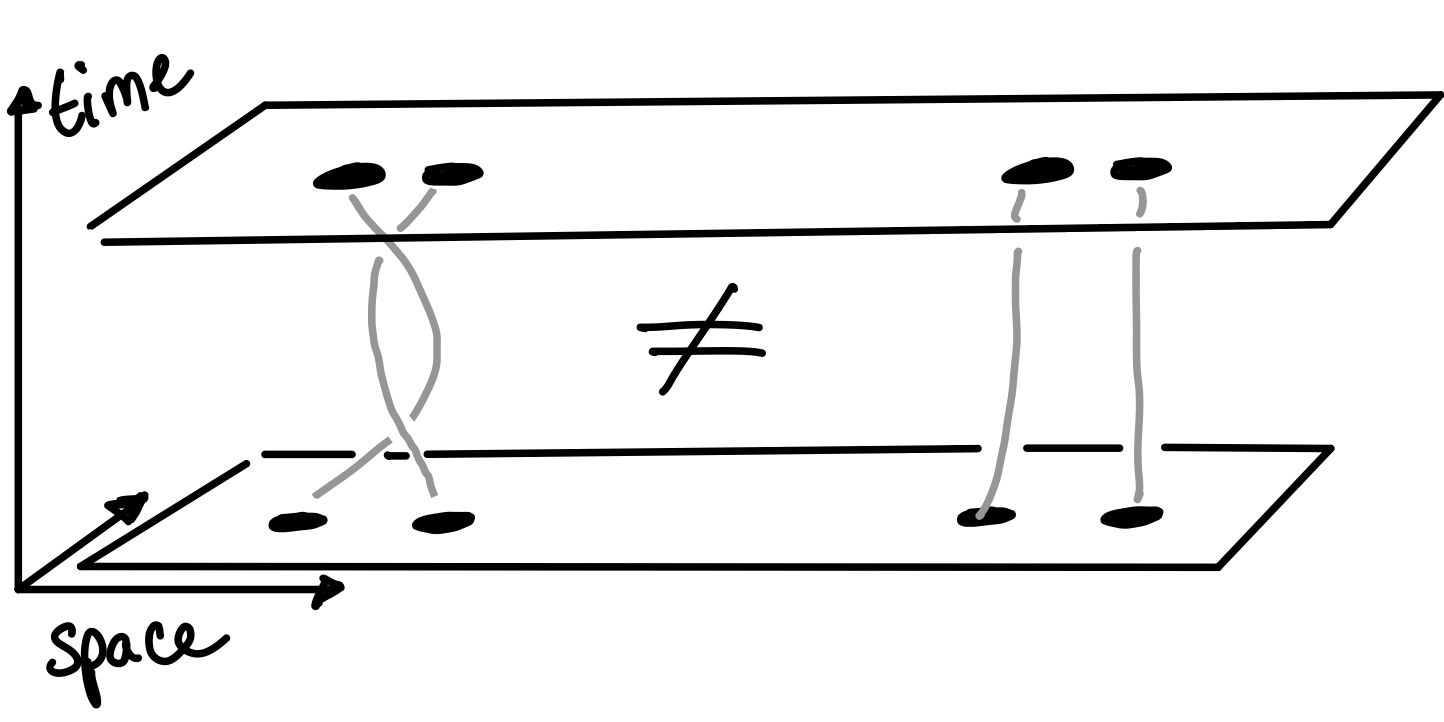
\includegraphics[width=0.71\textwidth,height=\textheight]{figure_code/amk_chapter/braiding.png}
\caption{}\label{fig:braiding}
}
\end{figure}

From this fact flows a whole new world of behaviours, now the quantum
state can aquire a phase factor \(e^{i\phi}\) upon exchange of two
identical particles, which we now call Anyons.

The Kitaev Model is a good demonstration of the connection beween Anyons
and topological degeneracy. In the Kitaev model we can create a pair of
vortices, move one around a non-contractable loop \(\mathcal{T}_{x/y}\)
and then anhilate them together. Without topology this should leave the
quantum state unchanged. Instead it moves us to another ground state in
a topologically degenerate ground state subspace. Practically speaking
it flips a dual line of bonds \(u_{jk}\) going around the loop which we
cannot undo with any gauge transformation made from \(D_j\) operators.

If the ground state subspace is multidimensional, quasiparticle exchange
can move us around in the space with an action corresponding to a
matrix. These matrices do not in general commmute and so these are known
as non-Abelian anyons.

From here things get even more complex, the Kitaev model has a
non-Abelian phase when exposed to a magnetic field, and the amorphous
Kitaev Model has a non-Abelian phase because of its broken chiral
symmetry.

The way that we have subdivided the Kitaev model into vortex sectors, we
have a neat separation beween vortices and fermionic excitations.
However if we looked at the full many body picture we would see that a
vortex caries with it a cloud of bound majorana states.

\begin{figure}
\hypertarget{fig:majorana_bound_states}{%
\centering
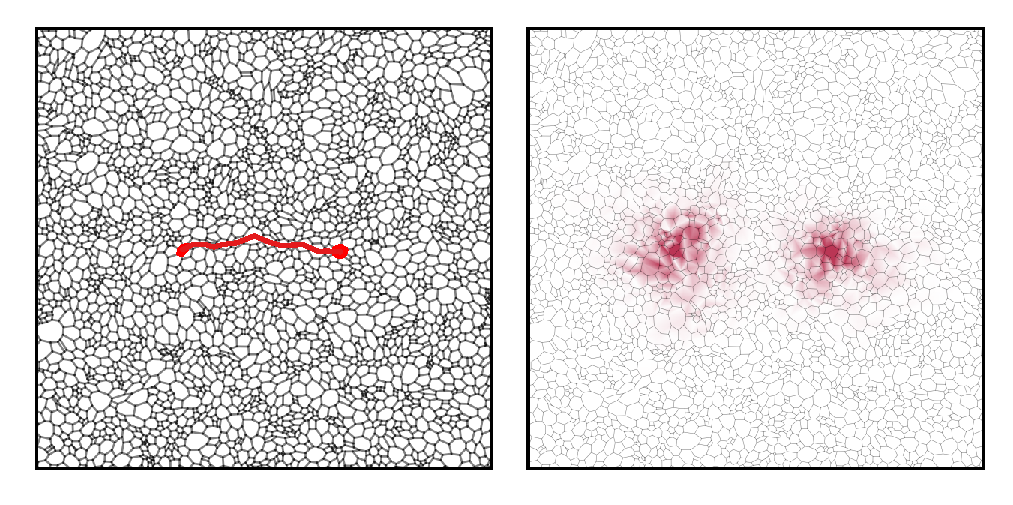
\includegraphics[width=1\textwidth,height=\textheight]{figure_code/amk_chapter/majorana_bound_states/majorana_bound_states.pdf}
\caption{(Left) A large amorphous lattice in the ground state save for a
single pair of vortices shown in red, separated by the string of bonds
that we flipped to create them. (Right) The density of the lowest energy
Majorana state in this vortex sector. The state is clearly bound to the
vortices.}\label{fig:majorana_bound_states}
}
\end{figure}

Consider two processes

\begin{enumerate}
\def\labelenumi{\arabic{enumi})}
\item
  We transport one half of a vortex pair around either the x or y loops
  of the torus before anhilating back to the ground state vortex sector
  \(\mathcal{T}_{x,y}\).
\item
  We flip a line of bond operators coresponding to measuring the flux
  through either the major or minor axes of the torus
  \(\mathcal{\Phi}_{x,y}\)
\end{enumerate}

\begin{figure}
\hypertarget{fig:loops_and_dual_loops}{%
\centering
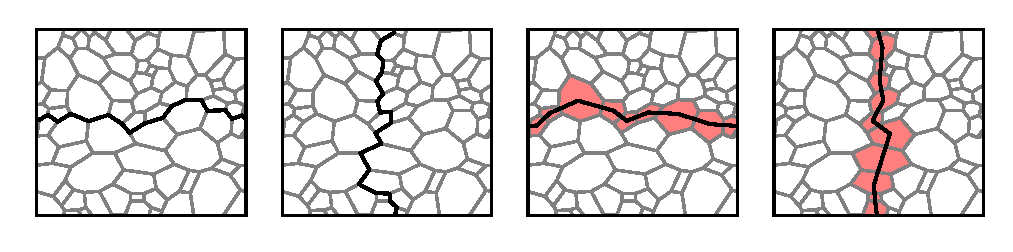
\includegraphics[width=1.14\textwidth,height=\textheight]{figure_code/amk_chapter/loops_and_dual_loops/loops_and_dual_loops.pdf}
\caption{(Left) The two topological flux operators of the toroidal
lattice, these don't correspond to any face of the lattice, but rather
measure flux that threads through the major and minor axes of the torus.
This shows a particular choice but any loop that crosses the boundary is
gauge equivalent to one of or the sum of these two loop. (Right) The two
ways to transport vortices around the diameters. These correspond to
creating a vortex pair, transporting one of them around the major or
minor diameters of the torus and then anhilating them
again.}\label{fig:loops_and_dual_loops}
}
\end{figure}

The plaquette operators \(\phi_i\) are associated with fluxes. Wilson
loops that wind the torus are associated with the fluxes through its two
diameters \(\mathcal{\Phi}_{x,y}\).

In the Abelian phase we can move a vortex along any path we like and
then when we bring them back together they will anhilate back to the
vacuum, where we understand `the vacuum' to refer to one of the ground
states, though not necesarily the same one we started in. We can use
this to get from the \((\Phi_x, \Phi_y) = (+1, +1)\) ground state and
construct the set \((+1, +1), (+1, -1), (-1, +1), (-1, -1)\).

\begin{figure}
\hypertarget{fig:topological_fluxes}{%
\centering
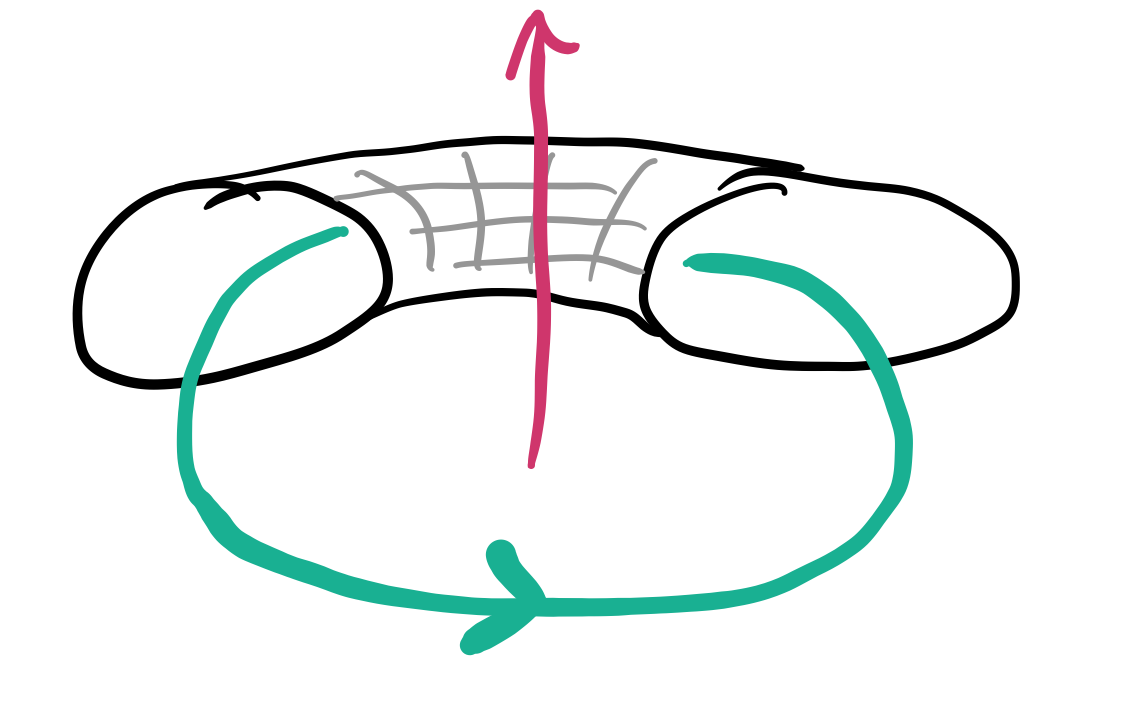
\includegraphics[width=0.57\textwidth,height=\textheight]{figure_code/amk_chapter/topological_fluxes.png}
\caption{Wilson loops that wind the major or minor diameters of the
torus measure flux winding through the hole of the donut/torus or
through the filling. If they made donuts that had both a jam filling and
a hole this analogy would be a lot easier to make
\textcite{parkerWhyDoesThis}.}\label{fig:topological_fluxes}
}
\end{figure}

However in the non-Abelian phase we have to wrangle with monodromy
\autocite{chungExplicitMonodromyMoore2007,oshikawaTopologicalDegeneracyNonAbelian2007}.
Monodromy is behaviour of objects as they move around a singularity.
This manifests here in that the identity of a vortex and cloud of
Majoranas can change as we wind them around the torus in such a way that
rather than anhilating to the vacuum the anhilate to create an excited
state instead of a ground state. This means we end up with only three
degenerate ground states in the non-Abelian phase
\((+1, +1), (+1, -1), (-1, +1)\)
\autocite[yaoAlgebraicSpinLiquid2009a]{chungTopologicalQuantumPhase2010}.
The way that this shows up concretly is that the projector enforces both
flux and fermion parity. When we wind a vortex around both
non-contractible loops of the torus, it flips the flux parity which
forces means we have to introduce a fermionic excitation to make the
state physical. Hence the process does not give a fourth ground state.

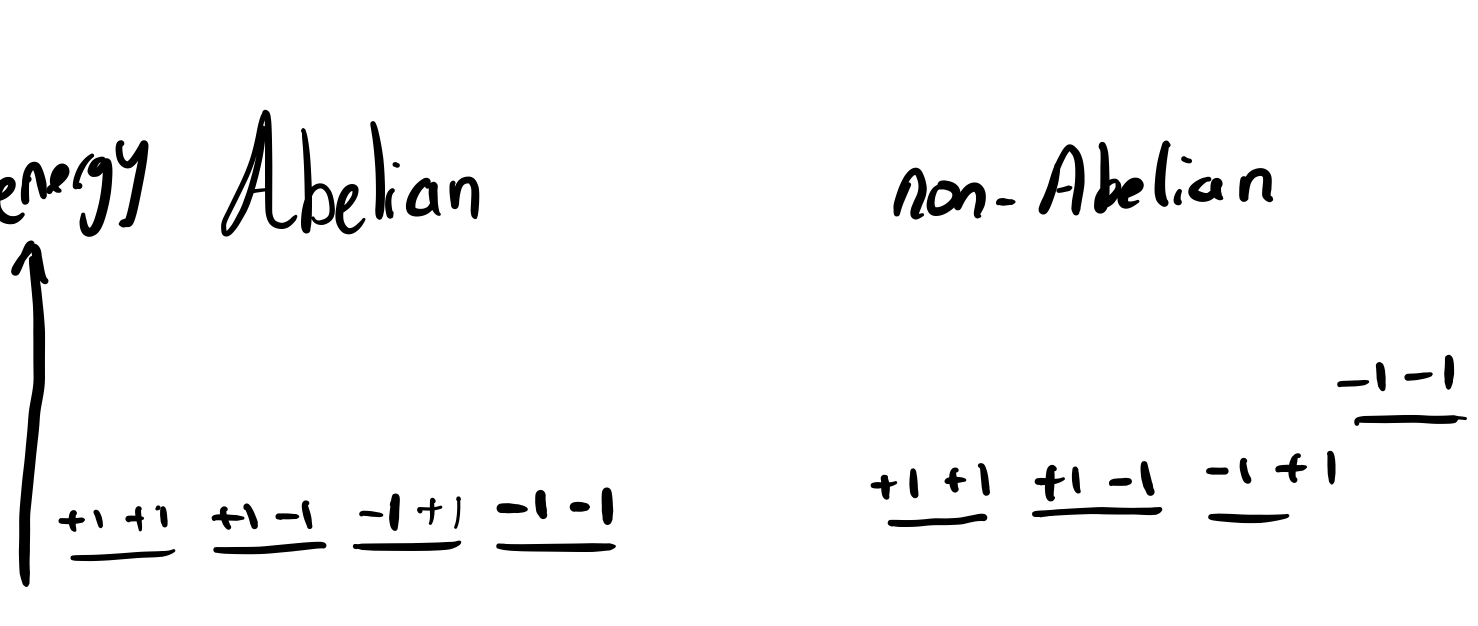
\includegraphics[width=0.86\textwidth,height=\textheight]{figure_code/amk_chapter/threefold_degeneracy.png}
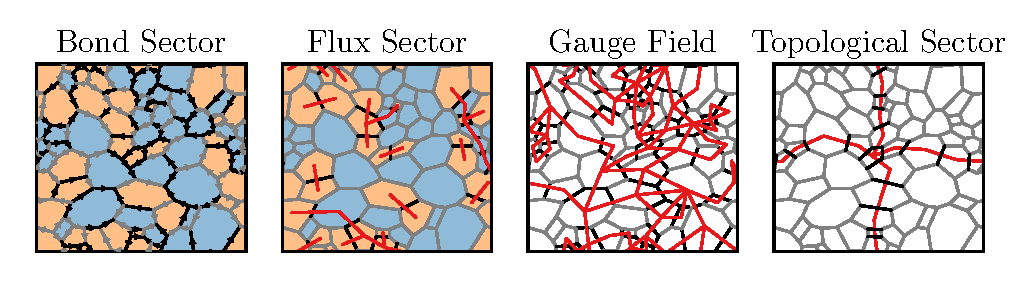
\includegraphics[width=1.14\textwidth,height=\textheight]{figure_code/amk_chapter/state_decomposition_animated/state_decomposition_animated.pdf}

One reason the topology has gained interest recently is there have
proposals to use this ground state degeneracy to implement both
passively fault tolerant and actively stabilised quantum computations
{[}\textcite{kitaevFaulttolerantQuantumComputation2003};
\textcite{poulinStabilizerFormalismOperator2005};
hastingsDynamicallyGeneratedLogical2021{]}.

\begin{Shaded}
\begin{Highlighting}[]
\OperatorTok{\%\%}\NormalTok{html}
\end{Highlighting}
\end{Shaded}

\hypertarget{methods}{%
\section{Methods}\label{methods}}

The practical implemntation of what is described in this section is
available as a Python package called Koala (Kitaev On Amorphous
LAttices) \textcite{tomImperialCMTHKoalaFirst2022} most of the figures
shown were generated with Koala.

\hypertarget{voronisation}{%
\subsection{Voronisation}\label{voronisation}}

In order to study the properties of the amorphous Kitaev model we need a
way to sample from the space of possible trivalent graphs.

A very simple way to do this is to use a Voronoi partition of the torus.
We start by sampling \emph{seed points} uniformly (or otherwise) on the
torus. We then compute the partition of the torus into regions closest
(with a Euclidean metric) to each seed point. The straight lines (if the
torus is flattened out) at the borders of these regions become the edges
of the new lattice and the points where they intersect beceme the
vertices.

The graph generated by a Voronoi partition of a two dimensional surface
is always planar meaning that no edges cross eachother when the graph is
embedded into the plane. It is also trivalent in the sense that every
vertex is connected to exactly three edges \textbf{cite}.

Ideally we might instead sample uniformly from the space of possible
trivalent graphs, and indeed there has been some work on how to do this
using a Markov Chain Monte Carlo approach
\textcite{alyamiUniformSamplingDirected2016}, however it does not
gurantee that the resulting graph is planar which we will need to ensure
that the edges can be 3-coloured.

In practice, we then use a standard algorithm
\textcite{barberQuickhullAlgorithmConvex1996} from scipy
\textcite{virtanenSciPyFundamentalAlgorithms2020a} which actually
computes the Voronoi partition of the plane. In order to compute the
Voronoi partition of the torus, I take the seed points and replicate
them into a repeating grid, either 3x3 (or for very small numbers of
seed points 5x5). I then identify edges in the output to construct a
lattice on the torus.

\begin{figure}
\hypertarget{fig:lattice_construction_animated}{%
\centering
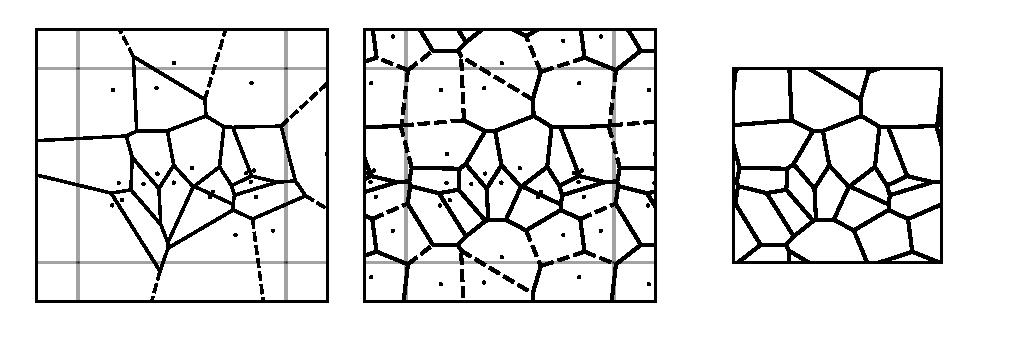
\includegraphics{figure_code/amk_chapter/lattice_construction_animated/lattice_construction_animated.pdf}
\caption{(Left) Lattice construction begins with the Voronoi partition
of the plane with respect to a set of seed points (black points) sampled
uniformly from \(\mathbb{R}^2\). (Center) However we actually want the
Voronoi partition of the torus so we tile the seed points into a three
by three grid. The boundaries of each tile are shown in light grey.
(Right) Finally we indentify edges correspond to each other across the
boundaries to produce a graph on the torus. An edge colouring is shown
here to help the reader identify corresponding
edges.}\label{fig:lattice_construction_animated}
}
\end{figure}

\hypertarget{graph-representation}{%
\subsection{Graph Representation}\label{graph-representation}}

We represent the graph structure with an ordered list of edges \((i,j)\)
so we can represent both directed and undirected graphs which is useful
for defining the sign of bond operators \(u_{ij} = - u_{ji}\).

\hypertarget{coloring-the-bonds}{%
\subsection{Coloring the Bonds}\label{coloring-the-bonds}}

The Kitaev model requires that each edge in the lattice be assigned a
label \(x\), \(y\) or \(z\) such that each vertex has exactly one edge
of each type connected to it. Let \(\Delta\) be the maximum degree of a
graph which in our case is 3. If \(\Delta > 3\) it is obviously not
possible to 3 color the edges but the general theory of when this is and
isn't possible for graphs with \(\Delta \leq 3\) is more subtle.

In the graph theory literature, graphs where all vertices have degree 3
are commonly called cubic graphs, there is no term for graphs with
maximum degree 3. Planar graphs are those that can be embedded onto the
plane without any edges crossing. Bridgeless graphs do not contain any
edges that, when removed, would partition the graph into disconnected
components.

It's important to be clear that this problem is different from that
considered by the famous 4 color theorem
\textcite{appelEveryPlanarMap1989} . The 4 color thorem is concerned
with assiging colours to the \textbf{vertices} of a graph such that no
vertices that share an edge are the same colour. Here we are concerned
with an edge colouring.

The four color theorem applies to planar graphs, those that can be
embedded onto the plane without any edges crossing. Here we are actually
concerned with Toroidal graphs which can be embedded onto the torus
without any edges crossing. In fact toroidal graphs require up to 7
colors \textcite{heawoodMapColouringTheorems} . The complete graph
\(K_7\) is a good example of a toroidal graph that requires 7 colours.

\(\Delta + 1\) colours are enough to edge-colour any graph and there is
an \(\mathcal{O}(mn)\) algorithm to do it for a graph with \(m\) edges
and \(n\) vertices \textcite{gEstimateChromaticClass1964}. Restricting
ourselves to graphs with \(\Delta = 3\) like ours, those can be
4-edge-coloured in linear time
\textcite{skulrattanakulchai4edgecoloringGraphsMaximum2002} .

It's trickier if we want to 3-edge-colour them however. Cubic, planar
bridgeless graphs can be 3-edge-coloured if and only if they can be
4-face-coloured \textcite{tait1880remarks} . For which there is an
\(\mathcal{O}(n^2)\) algorithm robertson1996efficiently . However it is
not clear whether this extends to cubic, \textbf{toroidal} bridgeless
graphs.

\hypertarget{face-colourablity-implies-3-edge-colourability}{%
\paragraph{4-face-colourablity implies
3-edge-colourability}\label{face-colourablity-implies-3-edge-colourability}}

The proof of that 4-face-colourablity implies 3-edge-colourability can
be sketched out quite easily: 1. Assume the faces of G can be 4-coloured
with labels (0,1,2,3) 2. Label each edge of G according to
\(i + j \mathrm{mod} 3\) where i and j are the labels of the face
adjacent to that edge. For each edge label there are two face label
pairs that do not share any face labels. i,e the edge label \(0\) can
come about either from faces \(0 + 3\) or \(1 + 2\).

\[\begin{aligned}
0 + 3 \;\mathrm{or}\; 1 + 2 &= 0 \;\mathrm{mod}\; 3\\ 
0 + 1 \;\mathrm{or}\; 2 + 3 &= 1 \;\mathrm{mod}\; 3\\
0 + 2 \;\mathrm{or}\;1 + 3 &= 2 \;\mathrm{mod}\; 3\\
\end{aligned}
\]

\begin{enumerate}
\def\labelenumi{\arabic{enumi}.}
\setcounter{enumi}{2}
\tightlist
\item
  In a cubic planar G, a vertex v in G is always part of 3 faces and the
  colors of those faces determines the colors of the edges that connect
  to v. The three faces must take three distinct colors from (0,1,2,3).
\item
  From there's easy to convince yourself that those three distinct face
  colours can never produce repeated edge colours according to the
  \(i+j \;\mathrm{mod}\; 3\) rule.
\end{enumerate}

This implies that all cubic planar graphs are 3-edge-colourable. It does
not apply to toroidcal graphs, however I have not yet generated a
voronoi lattices on the torus that is not 3-edge-colourable. This
suggests that perhaps voronoi lattices have additional structure that
makes them 3-edge-colourable. Intuitively, the kinds of toroidal graphs
that cannot be 3-edge-coloured look as if they could never be generated
by a voronoi partition with more than a few seed points.

\hypertarget{finding-lattice-colourings-in-practice-unfinished}{%
\subsubsection{Finding Lattice colourings in practice
(unfinished)}\label{finding-lattice-colourings-in-practice-unfinished}}

Some things are harder in theory than in practice. 3-edge-colouring
cubic toroidal graphs appears to be one of those things.

The approach I take is relatively standard in the computer science
community for solving NP problems computationally. I don't believe this
problem to be in NP but I tried it anyway.

The trick is to map the problem on into a Boolean Satisfiability `SAT'
problem, use an off the shelf solver for such problems then map the
problem back to the original domain. While SAT solvers are very general,
they are also highly optimised and they do seem to yield good results
for this problem.

SAT solvers encode problems as constraints on some number of boolean
variables \(x_i \in {0,1}\). The constraints must Conjunctive Normal
Form (CNF). CNF means the constraints are encoded as a set of clauses of
the form \[x_1 \;\textrm{or}\; \bar{x}_3 \;\textrm{or}\; x_5\] that
containt logical ORs of some subset of the variables where any of the
variables may also be logical NOT'd which I represent by over bars here.

A solution of the problem is one that makes all the clauses
simultaneously true.

I encode the edge colouring problem as a set of statements about a set
of boolean variables \(x_i \in {0,1}\). For \(B\) bonds we take the
\(3B\) variables \(x_{i\alpha}\) where \(x_{i\alpha} = 1\) indicates
that edge \(i\) has colour \(\alpha\).

For edge colouring graphs we need two kinds of constraints: 1. Each edge
is exactly one colour. 2. No neighbouring edges are the same color.

The first constraint is a kind of artifact of doing this mapping over to
boolean variables, the solver doesn't know anything about the structure
of the problem unless it is encoded into the variables.

The second constraint encodes the structure of the graph itself and can
be constructed easily from the adjacency matrix.

I'll fill in the encoding later but the gist is that we can give this to
a solver and get back: whether the problem is solveable, a solution or
all the possible solutions. Finding a solution is relatively fast, while
finding all the solutions is slower since there appear to be
exponentially many of them. Fig \ref{fig:multiple_colourings} shows some
examples.

\begin{figure}
\hypertarget{fig:multiple_colourings}{%
\centering
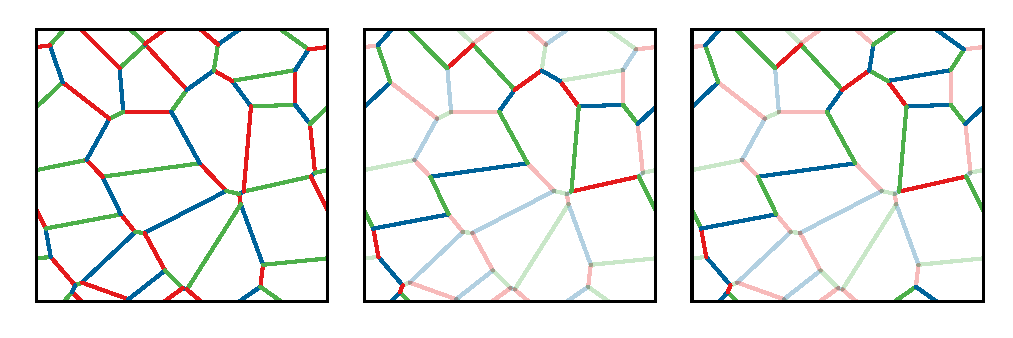
\includegraphics{figure_code/amk_chapter/multiple_colourings/multiple_colourings.pdf}
\caption{Three different valid 3-edge-colourings of amorphous lattices.
Colors that differ from the leftmost panel are
highlighted.}\label{fig:multiple_colourings}
}
\end{figure}

\hypertarget{mapping-between-flux-sectors-and-bond-sectors}{%
\subsection{Mapping between flux sectors and bond
sectors}\label{mapping-between-flux-sectors-and-bond-sectors}}

Constructing the Majorana representation of the model requires the
particular bond configuration \(u_{jk} = \pm 1\). However the large
number of gauge symmetries of the bond sector make it unwieldly to work
with. We therefore need a way to quickly map between bond sectors and
flux sectors.

Going from the bond sector to flux sector is easy since we can compute
it directly by taking the product of \(i u_{jk}\) around each plaquette
\[ \phi_i = \prod_{(j,k) \; \in \; \partial \phi_i} i u_{jk}\]

Going from flux sector to bond sector requires more thought however. The
algorithm I use is this:

\begin{enumerate}
\def\labelenumi{\arabic{enumi}.}
\item
  Fix the gauge by choosing some arbitrary \(u_{jk}\) configuration. In
  practice I use \(u_{jk} = +1\). This chooses an arbitrary one of the 4
  topological sectors.
\item
  Compute the current flux configuration and how it differs from the
  target one. Let's call an plaquette that differs from the target a
  defect.
\item
  Find any adjacent pairs of defects and flip the \(u_jk\) between them.
  This leaves a set of isolated defects.
\item
  Pair the defects up using a greedy algorithm.
\item
  Compute paths along the dual lattice between each pair of plaquettes.
  Flipping the corresponding set of \(u_{jk}\) transports one flux to
  the other and anhilates them.
\end{enumerate}

\begin{figure}
\hypertarget{fig:flux_finding}{%
\centering
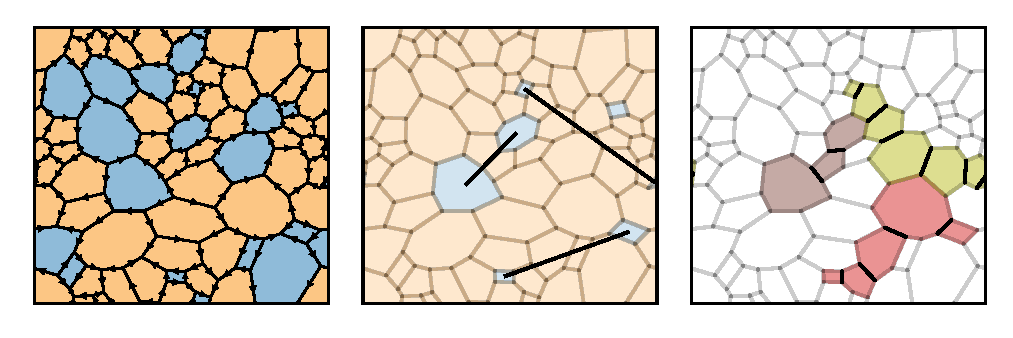
\includegraphics{figure_code/amk_chapter/flux_finding/flux_finding.pdf}
\caption{(Left) The ground state flux sector and bond sector for an
amorphous lattice. Bond arrows indicate the direction in which
\(u_{jk} = +1\). Plaquettes are coloured blue when \(\hat{\phi}_i = -1\)
(\(-i\)) for even (odd) plaquettes and orange when \(\hat{\phi}_i = +1\)
(\(+i\)) for even/odd plaquettes. (Centre) In order to transform this to
the target flux sector (all \(+1\)/\(+i\)) we first flip any \(u_{jk}\)
that are between two fluxes. This leaves a set of isolated fluxes that
need to be anhilated. These are then paired up as indicated by the black
lines. (Right) A* search is used to find paths (coloured plaquettes) on
the dual lattice between each pair of fluxes and the coresponding
\(u_{jk}\) (shown in black) are flipped. One flux has will remain
because the starting and target flux sectors differed by an odd number
of fluxes.}\label{fig:flux_finding}
}
\end{figure}

\hypertarget{results}{%
\section{Results}\label{results}}

\hypertarget{the-ground-state-flux-sector}{%
\subsection{The Ground State Flux Sector}\label{the-ground-state-flux-sector}}

Here I will discuss the numerical evidence that our guess for the ground state flux sector is correct. We will do this by enumerating all the flux sectors of many separate system realisations. However there are some issues we will need to address to make this argument work.

We have two seemingly irreconcilable problems. Finite size effects have a large energetic contribution for small systems \autocite{kitaevAnyonsExactlySolved2006} so we would like to perform our analysis for very large lattices. However for an amorphous system with \(N\) plaquettes, \(2N\) edges and \(3N\) vertices we have \(2^{N-1}\) flux sectors to check and diagonalisation scales with \(\mathcal{0}(N^3)\). That exponential scaling makes it infeasible to work with lattices much larger than \(16\) plaquettes.

To get around this we instead look at periodic systems with amorphous unit cells. For a similarly sized periodic system with \(A\) unit cells and \(B\) plaquettes in each unit cell where \(N \sim AB\) things get much better. We can use Bloch's theorem to diagonalise this system in about \(\mathcal{0}(A B^3)\) operations, and more importantly there are only \(2^{B-1}\) flux sectors to check.

We fully enumerated the flux sectors of \textasciitilde25,000 periodic systems with disordered unit cells of up to \(B = 16\) plaquettes and \(A = 100\) unit cells.

However, showing that our guess is correct for periodic systems with disordered unit cells is not quite convincing on its own. We have effectively removed longer-range disorder from our lattices.

The second part of the argument is to show that the energetic effect of introducing periodicity scales away as we go to larger system sizes and has already diminished to a small enough value at 16 plaquettes, which is indeed what we find.

From this we argue that the results for small periodic systems generalise to large amorphous systems. We perform this analysis for both the isotropic point (\(J^\alpha = 1\)), as well as in the toric code phase (\(J^x = J^y = 0.25, J^z = 1\)).

In the isotropic case (\(J^\alpha = 1\)), our conjecture correctly predicted the ground state flux sector for all of the lattices we tested.

For the toric code phase (\(J^x, J^y = 0.25, J^z = 1\)) all but around (\(\sim 0.5 \%\)) lattices had ground states conforming to our conjecture. In these cases, the energy difference between the true ground state and our prediction was on the order of \(10^{-6} J\). It is unclear whether this is a finite size effect or something else.

\hypertarget{spontaneous-chiral-symmetry-breaking}{%
\subsection{Spontaneous Chiral Symmetry Breaking}\label{spontaneous-chiral-symmetry-breaking}}

The spin Kitaev Hamiltonian is real and therefore has time reversal symmetry (TRS). However, the flux \(\phi_p\) through any plaquette with an odd number of sides has imaginary eigenvalues \(\pm i\). The ground state sector induces a relatively regular pattern for the imaginary fluxes with only a global two-fold chiral degeneracy.

Thus, states with a fixed flux sector spontaneously break time reversal symmetry. This was first described by Yao and Kivelson~for a translation invariant Kitaev model with odd sided plaquettes \autocite{Yao2011}.

So we have flux sectors that come in degenerate pairs, where time reversal is equivalent to inverting the flux through every odd plaquette, a general feature for lattices with odd plaquettes~\autocite{yaoExactChiralSpin2007,Peri2020}. This spontaneously broken symmetry avoids the need to explicitly break TRS with a magnetic field term as is done in the original honeycomb model.

\hypertarget{ground-state-phase-diagram}{%
\subsection{Ground State Phase Diagram}\label{ground-state-phase-diagram}}

As previously discussed, the standard Honeycomb model has a Abelian, gapped phase in the anisotropic region (the A phase) and is gapless in the isotropic region. The introduction of a magnetic field breaks the chiral symmetry, leading to the isotropic region becoming a gapped, non-Abelian phase, the B phase.

We set the energy scale by requiring that \(J_x + J_y + J_z = 1\), this restricts the 3D phase space down to an equilateral triangle that is convenient for diagrams. Imagine the cube defined by \(J_\alpha \in [0,1]\) being cut by the plane \(J_x + J_y + J_z = 1\), we plot the projection of that plane in diagrams like \cref{fig:phase_diagram}.

Similar to the Kitaev Honeycomb model with a magnetic field, we find that the amorphous model is only gapless along critical lines, see \cref{fig:phase_diagram} (Left).

Interestingly, the gap closing exists in only one of the four topological sectors, though this is certainly a finite size effect as the sectors must become degenerate in the thermodynamic limit. Nevertheless this could be a useful way to define the (0, 0) topological flux sector for the amorphous model.

In the honeycomb model, the phase boundaries are located on the straight lines \(|J^x| = |J^y| + |J^x|\) and permutations of \(x,y,z\), shown as dotted line on \textasciitilde{}\ref{fig:phase_diagram} (Right). We find that on the amorphous lattice these boundaries exhibit an inward curvature, similar to honeycomb Kitaev models with flux \autocite{Nasu_Thermal_2015} or bond \autocite{knolle_dynamics_2016} disorder.

\begin{figure}
\hypertarget{fig:phase_diagram}{%
\centering
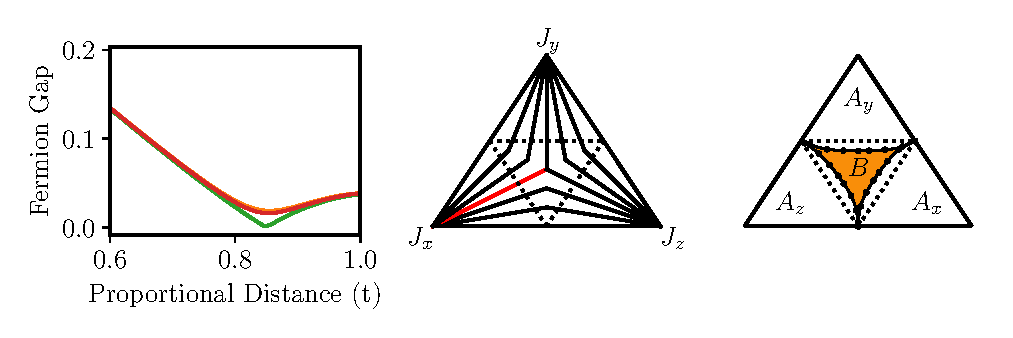
\includegraphics[width=1\textwidth,height=\textheight]{figure_code/amk_chapter/results/phase_diagram/phase_diagram.pdf}
\caption{(Center) We choose an energy scale for the Hamiltonian by setting \(J_x + J_y + J_z = 1\). This intersects a plane with the unit cube spanned by \(J_\alpha \in [0,1]\), giving a triangle with corners \((1,0,0), (0,1,0), (0,0,1)\). To compute critical lines efficiently in this space we evaluate the order parameter of interest along rays shooting from the corners. The ray highlighted in red defines the values of J used for the left figure. (Left) The fermion gap as a function of J for an amorphous system with 20 plaquettes, where the x axis is the position on the red line in the central figure from 0 to 1. For finite size systems the four topological sectors are not degenerate and only one of them has a true gap closing. (Right) The Abelian \(A_\alpha\) phases of the model and the non-Abelian B phase separated by critical lines where the fermion gap closes. Later we will show that the Chern number \(\nu\) changes from \(0\) to \(\pm 1\) from the A phases to the B phase. Indeed the gap \emph{must} close in order for the Chern number to change \textbf{citation}.}\label{fig:phase_diagram}
}
\end{figure}

\hypertarget{is-it-abelian-or-non-abelian}{%
\subsubsection{Is it Abelian or non-Abelian?}\label{is-it-abelian-or-non-abelian}}

The two phases of the amorphous model are clearly gapped, though later I'll double check this with finite size scaling.

The next question is: do these phases support excitations with Abelian or non-Abelian statistics? To answer that we turn to Chern numbers \autocite{berryQuantalPhaseFactors1984,simonHolonomyQuantumAdiabatic1983,thoulessQuantizedHallConductance1982}. As discussed earlier the Chern number is a quantity intimately linked to both the topological properties and the anyonic statistics of a model. Here we will make use of the fact that the Abelian/non-Abelian character of a model is linked to its Chern number \textbf{{[}citation{]}}. However the Chern number is only defined for the translation invariant case because it relies on integrals defined in k-space.

A family of real space generalisations of the Chern number that work for amorphous systems exist called local topological markers \autocite{bianco_mapping_2011,Hastings_Almost_2010,mitchellAmorphousTopologicalInsulators2018} and indeed Kitaev defines one in his original paper on the model \textcite{kitaevAnyonsExactlySolved2006}.

Here we use the crosshair marker of \textcite{peru_preprint} because it works well on smaller systems. We calculate the projector \(P = \sum_i |\psi_i\rangle \langle \psi_i|\) onto the occupied fermion eigenstates of the system in open boundary conditions. The projector encodes local information about the occupied eigenstates of the system and is typically exponentially localised \textbf{{[}cite{]}}. The name \emph{crosshair} comes from the fact that the marker is defined with respect to a particular point \((x_0, y_0)\) by step functions in x and y

\[\begin{aligned}
    \nu (x, y) = 4\pi \; \Im\; \mathrm{Tr}_{\mathrm{B}} 
    \left ( 
    \hat{P}\;\hat{\theta}(x-x_0)\;\hat{P}\;\hat{\theta}(y-y_0)\; \hat{P}
    \right ),
\end{aligned}\]

when the trace is taken over a region \(B\) around \((x_0, y_0)\) that is large enough to include local information about the system but does not come too close to the edges. If these conditions are met then then this quantity will be very close to quantised to the Chern number, see \cref{fig:phase_diagram_chern}.

We'll use the crosshair marker to assess the Abelian/non-Abelian character of the phases.

In the A phase of the amorphous model we find that \(\nu=0\) and hence the excitations have Abelian character, similar to the honeycomb model. This phase is thus the amorphous analogue of the Abelian toric-code quantum spin liquid \autocite{kitaev_fault-tolerant_2003}.

The B phase has \(\nu=\pm1\) so is a non-Abelian \emph{chiral spin liquid} (CSL) similar to that of the Yao-Kivelson model \autocite{yaoExactChiralSpin2007}. The CSL state is the the magnetic analogue of the fractional quantum Hall state \textbf{{[}cite{]}}. Hereafter we focus our attention on this phase.

\begin{figure}
\hypertarget{fig:phase_diagram_chern}{%
\centering
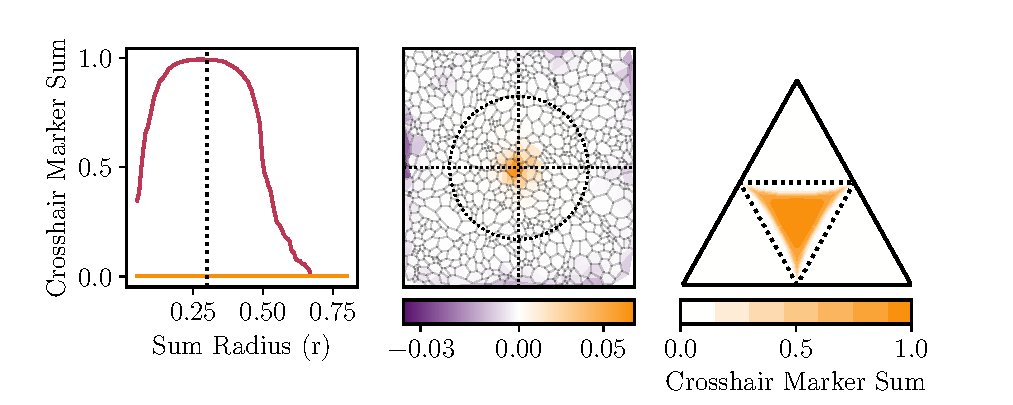
\includegraphics[width=1\textwidth,height=\textheight]{figure_code/amk_chapter/results/phase_diagram_chern/phase_diagram_chern.pdf}
\caption{(Center) The crosshair marker \textcite{peru_preprint}, a local topological marker, evaluated on the Amorphous Kitaev Model. The marker is defined around a point, denoted by the dotted crosshair. Information about the local topological properties of the system are encoded within a region around that point. (Left) Summing these contributions up to some finite radius (dotted line here, dotted circle in the centre) gives a generalised version of the Chern number for the system which becomes quantised in the thermodynamic limit. The radius must be chosen large enough to capture information about the local properties of the lattice while not so large as to include contributions from the edge states. The isotropic regime \(J_\alpha = 1\) in red has \(\nu = \pm 1\) implying it supports excitations with non-Abelian statistics, while the anisotropic regime in orange has \(\nu = \pm 0\) implying it has Abelian statistics. (Right) Extending this analysis to the whole \(J_\alpha\) phase diagram with fixed \(r = 0.3\) nicely confirms that the isotropic phase is non-Abelian.}\label{fig:phase_diagram_chern}
}
\end{figure}

\hypertarget{edge-modes}{%
\subsubsection{Edge Modes}\label{edge-modes}}

Chiral Spin Liquids support topological protected edge modes on open boundary conditions \autocite{qi_general_2006}. \cref{fig:edge_modes} shows the probability density of one such edge mode. It is near zero energy and exponentially localised to the boundary of the system. While the model is gapped in periodic boundary conditions (i.e on the torus) these edge modes appear in the gap when the boundary is cut.

The localization of the edge modes can be quantified by their inverse participation ratio (IPR), \[\mathrm{IPR} = \int d^2r|\psi(\mathbf{r})|^4  \propto L^{-\tau},\] where \(L\sim\sqrt{N}\) is the linear dimension of the amorphous lattices and \(\tau\) the dimensional scaling exponent of IPR. This is relevant because localised in-gap states do not participate in transport and hence do not turn band insulators into metals. It is only when the gap fills with extended states that we get a metallic state.

\begin{figure}
\hypertarget{fig:edge_modes}{%
\centering
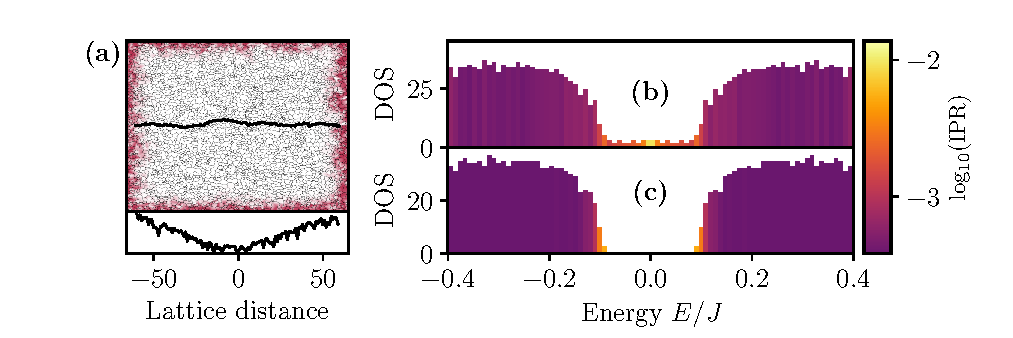
\includegraphics[width=1\textwidth,height=\textheight]{figure_code/amk_chapter/results/edge_modes/edge_modes.pdf}
\caption{(a) The density of one of the topologically protected edge states in the B phase. (Below) the log density plotted along the black path showing that the state is exponentially localised. (a)/(b) The density of states of the corresponding lattice in (a) periodic boundary conditions, (b) open boundary conditions. The colour of the bars shows the mean log IPR for each energy window. Cutting the boundary fills the gap with localised states.}\label{fig:edge_modes}
}
\end{figure}

\hypertarget{anderson-transition-to-a-thermal-metal}{%
\subsection{Anderson Transition to a Thermal Metal}\label{anderson-transition-to-a-thermal-metal}}

Previous work on the honeycomb model at finite temperature has shown that the B phase undergoes a thermal transition from a quantum spin liquid phase a to a \textbf{thermal metal} phase \autocite{selfThermallyInducedMetallic2019}.

This happens because at finite temperature, thermal fluctuations lead to spontaneous vortex-pair formation. As discussed previously these fluxes are dressed by Majorana bounds states and the composite object is an Ising-type non-Abelian anyon \autocite{Beenakker2013}. The interactions between these anyons are oscillatory similar to the RKKY exchange and decay exponentially with separation \autocite{Laumann2012,Lahtinen_2011,lahtinenTopologicalLiquidNucleation2012}. At sufficient density, the anyons hybridise to a macroscopically degenerate state known as \emph{thermal metal} \autocite{Laumann2012}. At close range the oscillatory behaviour of the interactions can be modelled by a random sign which forms the basis for a random matrix theory description of the thermal metal state.

The amorphous chiral spin liquid undergoes the same form of Anderson transition to a thermal metal state. Markov Chain Monte Carlo would be necessary to simulate this in full detail \autocite{selfThermallyInducedMetallic2019} but in order to avoid that complexity in the current work we instead opted to use vortex density \(\rho\) as a proxy for temperature.

We simply give each plaquette probability \(\rho\) of being a vortex, possibly with one additional adjustment to preserve overall vortex parity. This approximation is exact in the limits \(T = 0\) (corresponding to \(\rho = 0\)) and \(T \to \infty\) (corresponding to \(\rho = 0.5\)) while at intermediate temperatures there may be vortex-vortex correlations that are not captured by positioning vortices using uncorrelated random variables.

First we performed a finite size scaling to that the presence of a gap in the CSL ground state and absence of a gap in the thermal phase are both robust as we go to larger systems, see \cref{fig:fermion_gap_vs_L}.

\begin{figure}
\hypertarget{fig:fermion_gap_vs_L}{%
\centering
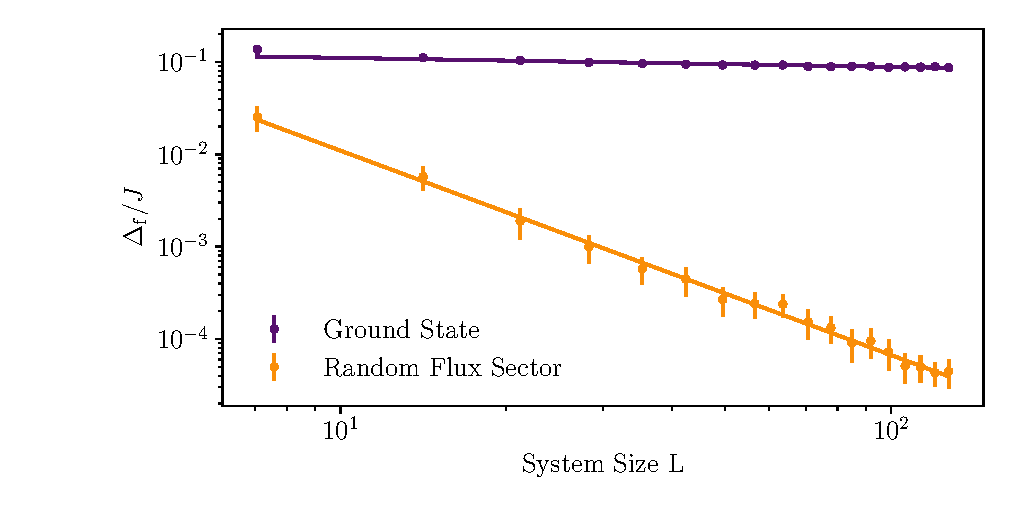
\includegraphics[width=1.14\textwidth,height=\textheight]{figure_code/amk_chapter/results/fermion_gap_vs_L/fermion_gap_vs_L.pdf}
\caption{Within a flux sector, the fermion gap \(\Delta_f\) measures the energy between the fermionic ground state and the first excited state. This graph shows the fermion gap as a function of system size for the ground state flux sector and for a configuration of random fluxes. We see that the disorder induced by an putting the Kitaev model on an amorphous lattice does not close the gap in the ground state. The gap closes in the flux disordered limit is good evidence that the system transitions to a gapless thermal metal state at high temperature. Each point shows an average over 100 lattice realisations. System size \(L\) is defined \(\sqrt{N}\) where N is the number of plaquettes in the system. Error bars shown are \(3\) times the standard error of the mean. The lines shown are fits of \(\tfrac{\Delta_f}{J} = aL ^ b\) with fit parameters: Ground State: \(a = 0.138 \pm 0.002, b = -0.0972 \pm 0.004\) Random Flux Sector: \(a = 1.8 \pm 0.2, b = -2.21 \pm 0.03\)}\label{fig:fermion_gap_vs_L}
}
\end{figure}

Next we evaluated the fermionic density of states (DOS), Inverse Participation Ratio (IPR) and IPR scaling exponent \(\tau\) as functions of the vortex density \(\rho\), see \cref{fig:DOS_vs_rho}. This leads to a nice picture of what happens as we raise the temperature of the system away from the gapped, insulating CSL phase. At small \(\rho\), states begin to populate the gap but they have \(\tau\approx0\), indicating that they are localised states pinned to the vortices, and the system remains insulating. At large \(\rho\), the in-gap states merge with the bulk band and become extensive, closing the gap, and the system transitions to the thermal metal phase.

\begin{figure}
\hypertarget{fig:DOS_vs_rho}{%
\centering
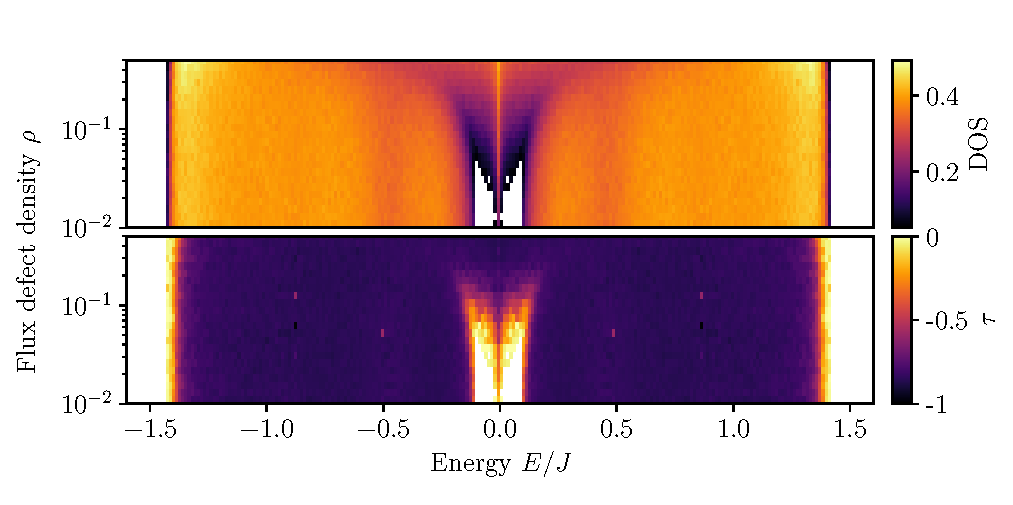
\includegraphics[width=1\textwidth,height=\textheight]{figure_code/amk_chapter/results/DOS_vs_rho/DOS_vs_rho.pdf}
\caption{(Top) Density of states and (Bottom) scaling exponent \(\tau\) of the amorphous Kitaev model as a vortex density \(\rho\) is increased. The scaling exponent \(\tau\) is the exponent with which the inverse participation ratio scales with system size. It gives a measure of the degree of localisation of the states in each \((E/J, \rho)\) bin. At zero \(\rho\) we have the gapped ground state. At small \(\rho\), states begin to populate the gap. These states have \(\tau\approx0\), indicating that they are localised states pinned to fluxes, and the system remains insulating. As \(\rho\) increases further, the in-gap states merge with the bulk band and become extensive, fully closing the gap, and the system transitions to a thermal metal phase.}\label{fig:DOS_vs_rho}
}
\end{figure}

The thermal metal phase has a signature logarithmic divergence at zero energy and oscillations in the DOS. These signatures can be shown to occur by a recursive argument that involves mapping the original model onto a Majorana model with interactions that take random signs which can itself be mapped onto a coarser lattice with lower energy excitations and so on. This can be repeating indefinitely, showing the model must have excitations at arbitrarily low energies in the thermodynamic limit \autocite{bocquet_disordered_2000,selfThermallyInducedMetallic2019}.

These signatures for our model and for the honeycomb model are shown in \cref{fig:DOS_oscillations}. They do not occur in the honeycomb model unless the chiral symmetry is broken by a magnetic field.

\begin{figure}
\hypertarget{fig:DOS_oscillations}{%
\centering
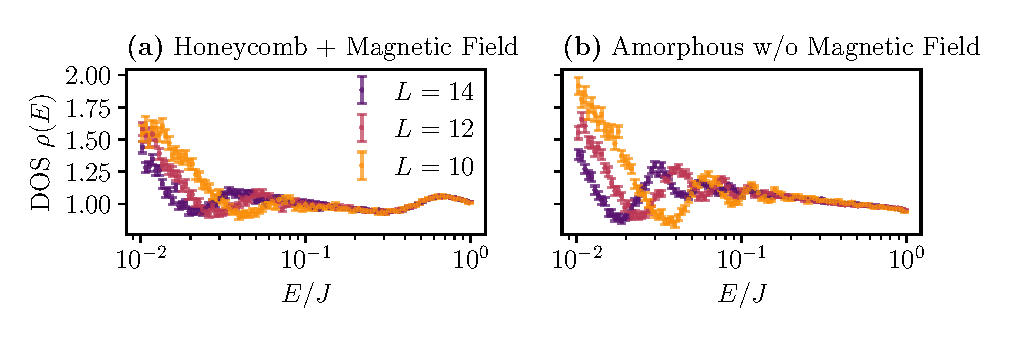
\includegraphics[width=1\textwidth,height=\textheight]{figure_code/amk_chapter/results/DOS_oscillations/DOS_oscillations.pdf}
\caption{Density of states at high temperature showing the logarithmic divergence at zero energy and oscillations characteristic of the thermal metal state \autocite{bocquet_disordered_2000,selfThermallyInducedMetallic2019}. (a) shows the honeycomb lattice model in the B phase with magnetic field, while (b) shows that our model transitions to a thermal metal phase without an external magnetic field but rather due to the spontaneous chiral symmetry breaking. In both plots the density of vortices is \(\rho = 0.5\) corresponding to the \(T = \infty\) limit.}\label{fig:DOS_oscillations}
}
\end{figure}

\hypertarget{conclusion}{%
\section{Conclusion}\label{conclusion}}

In this chapter we have looked at an extension of the Kitaev honeycomb model to amorphous lattices with coordination number three. We discussed a method to construct arbitrary trivalent lattices using Voronoi partitions, how to embed them onto the torus and how to edge-colour them using a SAT solver.

We provided extensive numerical evidence that the ground state flux sector of the model is given by a simply function of the number of sides of each plaquette backed up by an analysis of the energetic finite size effects.

We found two quantum spin liquid phases that can be distinguished using a real-space generalisation of the Chern number. We showed that via finite size scaling that these phases are robustly gapped. The presence of odd-sided plaquettes on these lattices let to a spontaneous breaking of time reversal symmetry, leading to the emergence of a chiral spin liquid phase.

Finally we showed evidence that the amorphous system undergoes an Anderson transition to a thermal metal phase, driven by the proliferation of vortices with increasing temperature.

\hypertarget{discussion}{%
\section{Discussion}\label{discussion}}

\hypertarget{limits-of-the-ground-state-conjecture}{%
\subsection{Limits of the ground state conjecture}\label{limits-of-the-ground-state-conjecture}}

We found a small number of lattices for which the ground state conjecture did not correctly predict the true ground state flux sector. I see two possibilities for what could cause this.

Firstly it could be a a finite size effect that is amplified by certain rare lattice configurations. It would be interesting to try to elucidate what lattice features are present when the ground state conjecture fails.

Alternatively, it might be telling that the ground state conjecture failed in the toric code A phase where the couplings are anisotropic. We showed that the colouring does not matter in the B phase. However an avenue that I did not explore was whether the particular choice of colouring for a lattice affects the physical properties in the toric code A phase. It is possible that some property of the particular colouring chosen is what leads to failure of the ground state conjecture here.

\hypertarget{outlook}{%
\section{Outlook}\label{outlook}}

This exactly solvable chiral QSL provides a first example of a topological quantum many-body phase in amorphous magnets, which raises a number of questions for future research.

\hypertarget{experimental-realisations-and-signatures}{%
\subsection{Experimental Realisations and Signatures}\label{experimental-realisations-and-signatures}}

The obvious question is whether amorphous Kitaev materials could be physically realised.

Most crystals can as exists in a metastable amorphous state if they are cooled rapidly, freezing them into a disordered configuration \autocite{Weaire1976,Petrakovski1981,Kaneyoshi2018}. Indeed quenching has been used by humans to control the hardness of steel or iron for thousands of years. It would therefore be interesting to study amorphous version of candidate Kitaev materials \textcite{trebstKitaevMaterials2022} such as \(\alpha-\textrm{RuCl}_3\) to see whether they maintain even approximate fixed coordination number locally as is the case with amorphous Silicon and Germanium \autocite{Weaire1971,betteridge1973possible}.

Looking instead at more engineered realisation, metal organic frameworks have been shown to be capable of forming amorphous lattices~\autocite{bennett2014amorphous} and there are recent proposals for realizing strong Kitaev interactions~\autocite{yamadaDesigningKitaevSpin2017} as well as reports of QSL behavior~\autocite{misumiQuantumSpinLiquid2020}.

\hypertarget{generalisations}{%
\subsection{Generalisations}\label{generalisations}}

The model presented here could be generalized in several ways.

First, it would be interesting to study the stability of the chiral amorphous Kitaev QSL with respect to perturbations~\autocite{Rau2014,Chaloupka2010,Chaloupka2013,Chaloupka2015,Winter2016}.

Second, one could investigate whether a QSL phase may exist for for other models defined on amorphous lattices. For example, in real materials, there will generally be an additional small Heisenberg term \[H_{KH} =  - \sum_{\langle j,k\rangle_\alpha} J^{\alpha}\sigma_j^{\alpha}\sigma_k^{\alpha} + \sigma_j\sigma_k\] With a view to more realistic prospects of observation, it would be interesting to see if the properties of the Kitaev-Heisenberg model generalise from the honeycomb to the amorphous case{[}\textcite{Chaloupka2010}; \textcite{Chaloupka2015}; \textcite{Jackeli2009}; \textcite{Kalmeyer1989}; \textcite{manousakisSpinTextonehalfHeisenberg1991};{]}.

Finally it might be possible to look at generalizations to higher-spin models or those on random networks with different coordination numbers \autocite{Baskaran2008,Yao2009,Nussinov2009,Yao2011,Chua2011,Natori2020,Chulliparambil2020,Chulliparambil2021,Seifert2020,WangHaoranPRB2021,Wu2009}

Overall, there has been surprisingly little research on amorphous quantum many body phases albeit material candidates aplenty. We expect our exact chiral amorphous spin liquid to find many generalisation to realistic amorphous quantum magnets and beyond.


% \chapter{Conclusion \& Discussion}
% \appendix
%     % \includepdf[pages=-]{APS_copyright_permission.pdf}

\addcontentsline{toc}{chapter}{Bibliography}
\printbibliography
\addcontentsline{toc}{chapter}{Copyright}
% \includepdf[pages=-]{5_Appendices/APS_copyright_permission.pdf}

\end{document}